\documentclass[10pt,a4paper]{report}

\usepackage[utf8]{inputenc}
\usepackage[T1]{fontenc}
\usepackage[english]{babel}
\usepackage[left=2.5cm,top=1.5cm,right=2.5cm,bottom=2cm]{geometry}

\usepackage{amsmath}
\usepackage{amsfonts}
\usepackage{amssymb}
\usepackage{amsopn}
\usepackage{amsthm}
\usepackage[hidelinks]{hyperref}
\usepackage{cleveref}
\usepackage{fancyvrb}
\usepackage{tikz}
\usepackage[justification=centering]{caption}
% \patchcmd{\thebibliography}{\chapter*}{\section*}{}{}
\usepackage[super]{nth}
\usepackage{textcomp}
\usepackage{enumitem}
\usepackage{doi}
\usepackage{mathrsfs}
\usepackage{siunitx}
\setlist{nosep}
% \usepackage[justification=justified,singlelinecheck=false]{caption}
\usepackage{subcaption}


\theoremstyle{plain}
\newtheorem{thm}{Theorem}[chapter]
\newtheorem{prop}[thm]{Property}
\newtheorem{lem}[thm]{Lemma}
\newtheorem{cor}{Corollary}[thm]

\theoremstyle{definition}
\newtheorem{defn}{Definition}[chapter]
\newtheorem{axi}{Axiom}[chapter]
\newtheorem{eqn}[thm]{Equation}

\theoremstyle{remark}
\newtheorem*{rem}{Remark}


\setcounter{secnumdepth}{3}
\setcounter{tocdepth}{1}
%\renewcommand\thesection{\arabic{section}}

\newcommand{\R}{\ensuremath{\mathbb{R}}}
\newcommand{\Rb}{\ensuremath{\overline{\mathbb{R}}}}
\newcommand{\N}{\ensuremath{\mathbb{N}}}
\newcommand{\Q}{\ensuremath{\mathbb{Q}}}
\newcommand{\Z}{\ensuremath{\mathbb{Z}}}
\newcommand{\C}{\ensuremath{\mathbb{C}}}
\newcommand{\U}{\ensuremath{\mathbb{U}}}
\newcommand{\F}{\ensuremath{\mathbb{F}}}
\newcommand{\K}{\ensuremath{\mathbb{K}}}
\newcommand{\TODO}{\textbf{TODO}}


\newcommand\eqdef{\stackrel{\mathclap{\mbox{\tiny def}}}{=}}


\sisetup{inter-unit-product=\ensuremath{{}\cdot{}}}

\newcommand{\ket}[1]{|#1\rangle}
\newcommand{\bra}[1]{\langle#1|}
\newcommand{\braket}[2]{\langle#1|#2\rangle}

\newcommand{\dd}{\mathrm{d}}
\newcommand{\der}[2]{\frac{\dd{#1}}{\dd{#2}}}
\newcommand{\dern}[3]{\frac{\dd^{#3} #1}{\dd{#2}^{#3}}}
\newcommand{\dpar}[2]{\frac{\partial{#1}}{\partial{#2}}}
\newcommand{\dparn}[3]{\frac{\partial^{#3} {#1}}{\partial{#2}^{#3}}}

\renewcommand{\geq}{\geqslant}
\renewcommand{\leq}{\leqslant}

\newcommand{\mat}[1]{\begin{pmatrix}#1\end{pmatrix}}
\newcommand{\bs}{\boldsymbol}

\DeclareMathOperator{\cov}{cov}
\DeclareMathOperator{\Tr}{Tr}
\DeclareMathOperator{\argmax}{arg\,max}
\DeclareMathOperator{\argmin}{arg\,min}
\DeclareMathOperator{\rk}{rk}
\DeclareMathOperator{\Span}{Span}
\DeclareMathOperator{\dom}{dom}


\newcommand{\class}[1]{{\mathscr{C}^{#1}}}

\newcommand{\trnorm}[1]{\frac{#1}{\Tr\left({#1}\right)}}




\newcommand{\ml}{_{M\!L}}


\newcommand{\maxim}[3]{\begin{cases}
    \mathbf{maximize}\,\quad #1& \mathbf{on}\; #2\\
    \mathbf{subject\;to}\quad #3
  \end{cases}}
\newcommand{\maximf}[2]{\begin{cases}
    \mathbf{maximize}\,\quad #1& \mathbf{on}\; #2
  \end{cases}}
\newcommand{\maxima}[3]{\begin{cases}
    \mathbf{maximize}\,\quad #1& \mathbf{on}\; #2\\
    \mathbf{subject\;to}\quad \begin{aligned}[t]#3\end{aligned}
  \end{cases}}

\newcommand{\minim}[3]{\begin{cases}
    \mathbf{minimize}\;\,\quad #1& \mathbf{on}\; #2\\
    \mathbf{subject\;to}\quad #3
  \end{cases}}
\newcommand{\minimf}[2]{\begin{cases}
    \mathbf{minimize}\,\quad #1& \mathbf{on}\; #2
  \end{cases}}
\newcommand{\minima}[3]{\begin{cases}
    \mathbf{minimize}\;\,\quad #1& \mathbf{on}\; #2\\
    \mathbf{subject\;to}\quad \begin{aligned}[t]#3\end{aligned}
  \end{cases}}

\newcommand{\gap}{\hspace{1.5cm}}
\newcommand{\twoline}{\vphantom{\frac\int\int}}



% \usepackage{titlesec}
% \titleformat{\chapter}[hang]

% \makeatletter
% \def\@makechapterhead#1{%
%   \vspace*{50\p@}% %%% removed!
%   {\parindent \z@ \raggedright \normalfont
%     \ifnum \c@secnumdepth >\m@ne
%         \huge\bfseries \@chapapp\space \thechapter
%         \par\nobreak
%         \vskip 10\p@
%     \fi
%     \interlinepenalty\@M
%     \Huge \bfseries #1\par\nobreak
%     \vskip 30\p@
%   }}
% \def\@makeschapterhead#1{%
%   \vspace*{50\p@}% %%% removed!
%   {\parindent \z@ \raggedright
%     \normalfont
%     \interlinepenalty\@M
%     \Huge \bfseries  #1\par\nobreak
%     \vskip 30\p@
%   }}
% \makeatother

% \usepackage{titlesec}
% \titlespacing*{\section}{0pt}{.7\baselineskip}{.5\baselineskip}
% \titlespacing*{\subsection}{0pt}{.4\baselineskip}{.3\baselineskip}

\graphicspath{{../img/}}

\title{Error estimation in maximum-likelihood reconstruction for quantum state tomography}
\author{Thibaut Pérami}

\makeatletter
\hypersetup{
  pdftitle = {\@title},
  pdfauthor = {\@author},
  pdfsubject = {Quantum state tomography}
}
\makeatother

\begin{document}

\begin{titlepage}
  \centering
  {\scshape\huge École Normale Supérieure \par}
  \vspace{0.3cm}
  {\scshape\Large Department of Mathematics and their Applications (DMA) \par}
  \vspace{3cm}
  {\Huge\bfseries Error estimation in maximum likelihood reconstruction for
    quantum state tomography \par}
  \vspace{0.5cm}
  {\scshape\Large Internship report\par}
  \vspace{3cm}
  {\LARGE Thibaut \textsc{Pérami}\par}
  \vfill
  {
    \large
    supervised by\par
    Igor \textsc{Dotsenko}\par
    and\par
    Pierre \textsc{Rouchon}\par
  in\par
  LKB, Collège de France
  }

  \vfill

  % Bottom of the page
  {\Large September 2, 2019\par}
\end{titlepage}

\newcommand{\fset}{\ensuremath{\mathop{\text{\textquotesingle}}}}




\chapter*{Abstract}
\addcontentsline{toc}{chapter}{Abstract}
In this report, I explain the content of my internship with Igor Dotsenko and
Pierre Rouchon at the Laboratoire Kastler Brossel in the Collège de France. I studied quantum
electrodynamics in cavities, and in particular an experiment conducted by another
intern, Luis Najera. He developed a way to transfer energy from a colder atom to a
hotter cavity by using quantum manipulation with resonant Rabi oscillations. In
order to extract main results from this experiment, we use quantum state tomography, in
particular maximum log-likelihood estimation. In their original state of the art, when I
arrived, the results of such estimations were only proven when observing usual
quantum observable. However, Luis was studying quantum thermodynamics and thus
needed to use among other the von-Neumann entropy of the reconstructed quantum states. I thus
extended the proofs of such estimation to handle that case. Additionally, I also experimented
with a method to solve a problem of insufficient measurement on a quantum system.




\vfill

\paragraph{\Huge Notations}

\addcontentsline{toc}{chapter}{Notations}

\

\vspace{1.5cm}

\begin{itemize}
  \item $\lambda,\mu,x,w,n$: scalar, generic vector and function are normal
    letters.
    Usually, I try to use greek letters for scalars, but this is not always the case.
  \item $A,B,H$: quantum operator or more generally matrices are capital letters
  \item $\bs u, \bs E$, 3D vectors or 3D quantum operator are in bold, capital
    letter for operators.
  \item $\mathcal{E}$: curved letter are generally for sets.
  \item $\mathbb H, \mathbb E$: Apart from usual sets ($\R,\C,\N,\Z$) doubled
    letters represent super-operator i.e operators from matrices to matrices.
  \item $x^*$: complex conjugate of $x$.
  \item $A^t$: transposed matrix of $A$.
  \item $A^\dagger$: transpose conjugate of $A$: $A^\dagger = {(A^t)}^*$.
  \item $x \cdot y$: The real scalar product $\sum_i x_i y_i$. On complex vectors it
    will still be the same formula and thus $x^* \cdot y = \braket x y$.
  \item $\braket x y$: complex scalar product, semi-linear to left i.e.\ physicist convention.
  \item $\ket x$, $\bra x$: I use Dirac bra-ket notation. In addition, if $A$
    is a matrix, $\ket A$ will be a column vector
    representing the matrix.
  \item $x > y$: for two vector of $\R^n$, $x > y$ means component wise inequality
  \item $A > B$: $A - B$ is Hermitian positive definite. (semidefinite for $A
    \geq B$)
  \item $\mathcal{H}$: A Hilbert space
  \item $\mathcal{L}(\mathcal{H})$: The set of operator a $\mathcal{H}$
  \item $\mathcal{L}(\mathcal{H}, \mathcal{H}')$: The set of operator from
    $\mathcal{H}$ to $\mathcal{H}'$.
  \item $\mathcal{U}(\mathcal{H})$: The set of unitary matrice on $\mathcal{H}$
    (orthogonal if $\mathcal{H}$ is a real vector space)
  \item $\mathcal{O}(\mathcal{H})$: The set of observable i.e of Hermitian matrice on $\mathcal{H}$
  \item $\mathcal{S}(\mathcal{H})$: The set of real symmetric matrices.
  \item $\mathcal{D}(\mathcal{H})$: The set of density matrices.
  \item $\R_+$, $\mathcal{O}_+(\mathcal{H})$: The set of non-negative real, of
    positive semi-definite hermitian matrices.
  \item $\nabla f$: gradient on mono-result function, but also jacobian matrix
    on multi-result function
  \item $\nabla^2 f$: Hessian matrix
  \item $\dpar f x, \partial_x f$: Partial derivative. If $x$ is a vector, it is
    a partial gradient or a partial jacobian matrix.
  \item $\dparn f x 2$: 2nd partial derivative, but may be a partial Hessian if
    $x$ is a vector
\end{itemize}

\tableofcontents

\chapter*{Introduction}
% \pagenumbering{arabic}
\addcontentsline{toc}{chapter}{Introduction}

This report details my internship with Pierre Rouchon and Igor Dotsenko on
quantum state tomography by maximum-likelihood reconstruction (MaxLike). It was done mainly at
the Laboratory Kastler-Brosel (LKB) in the Collège de France.

The goal of quantum state tomography is to find a way to reconstruct the state of
a quantum system from several direct or indirect measurements on it. In some cases
these measurements do not modify the state of the system and are called
quantum non-destructive (QND) measurement.

The specific physical project on which I worked with Igor Dotsenko is the
internship project of Luis Najera on quantum thermodynamics in the case of
atom-cavity interaction in quantum optics. More precisely, we send a circular
Rydberg atom in a resonant cavity containing several photon field. The state of the cavity is
thermal i.e it follows the Bose-Einstein distribution. The atom then interacts
with the cavity. If the atom is in a thermal state of its two atomic levels, that
are at the same frequency than the cavity, then a thermal exchange will occur in
the expected way. However if we pump one of the atom's state in a hidden
state, like a Maxwell's demon, we can apparently break the second law of thermodynamics and make
a cold atom give heat to a hotter cavity.

In order to study this experiment, we need to measure the state of the cavity.
That state cannot be measured directly, so we reconstruct it by quantum state tomography using
maximum-likelihood estimation. This construction takes into account all the
measurements made and deduces a density matrix. To find it, one needs to solve a
convex optimisation problem on the set of density matrices (Hermitian positive
definite matrices of trace 1). This was done using a gradient descent method with
projection of the gradient on the domain.

The estimated state is usually not a pure state because the reconstruction
comes from a state that has been prepared several times.
All the prepared states are slightly different.
Furthermore, other factors like measurement imperfections and decoherent
relaxation decrease the precision of the reconstruction.

With these measurements, we can now get and interpret the results of our Maxwell's
demon experiment. However, to be able to interpret measurement, we need to know
the error on the reconstructed state. The original proofs in~\cite{SPRAL17} on
tomography only provide the standard deviation of usual quantum observables which
are linear in the density matrix. However, to perform our analysis of the second law,
we need to evaluate the error of the estimated entropy.

In order to do that, I first tried a Monte-Carlo algorithm and used the
distribution around the estimated value to sample the examined function. I could
then deduce a mean and a standard deviation. Later, I improved the proofs
of~\cite{SPRAL17} to show that evaluating the function on the estimator is
indeed asymptotically the average of the function around the estimator. I could
then also get an analytic value of the standard deviation around any
function of the density matrix. Additionally I also worked on fixing convergence
problems when the information given by the experiment is incomplete.

In the end we get error bars on our plots and we are able to determine which
points were, within their error bars, consistent with the theoretical description
of our Maxwell's demon experiment and which were not.

\

This report alternates maths and physics. The odd chapters are about the physical
part of the internship and the even ones about maths. The five first chapters are
about my understanding of prior work that I had to do in order to do what I did.
The last two describe my personal contributions.

In Chapter 1, I present the experiment, its formal modelisation and why we need
the quantum state tomography. In Chapter 2,
I explain the basics of maximum likelihood reconstruction and then I show in
Chapter 3 how this method is applied to our particular case. In Chapter 4, I show
how to solve the convex optimization problem that appeared. Then I present the
results obtained before I arrived in Chapter 5. In Chapter 6, I
explain what I did for computing error bars of a non-linear function and some other work.
The final results are given in Chapter 7.

\vfill



\chapter{Experimental setup and goal}

In this chapter I expect the reader to know the basics of quantum mechanics,
Hilbert spaces and
the Schrödinger equation. I will present the basic quantum electrodynamics
concepts needed to understand the experiment, and the experiment itself.
Everywhere in my report I will use the usual bra-ket notation
and, therefore, a scalar product linear to the right.

I will first schematically describe the experiment setup and then quickly dive
into some experimental details. I'll finish by explaining why the state
reconstruction is needed.

\section{Basic setup description}

In this section I describe the experiment I worked with at the LKB.\@ This
experiment studies the interaction between Rydberg circular atoms and light in
superconducting cavities.
We produce Rydberg atoms in a known circular state, then we send them through a
cavity containing a very small number of photons (usually less than
eight). The atom then goes through a detector that ideally performs projective
measurement of the state. The atoms can be tuned via Stark effect so the
interaction can be resonant (the cavity frequency correspond to a gap between
atomic states) or dispersive (the frequency and the gap do not match).

I will present the formalism for each component and then detail the formalism of
their interaction. The goal of the experiment is to study quantum
thermodynamics. In particular, with the right manipulation of the quantum state
of an atom, we can force it to give heat to the cavity (emit a photon) even if the atom
is colder than the cavity. I will define the notion of temperature of a single
atom later.

Most of the formulas come from the chapter 3 of~\cite{Har06} and the first part
of~\cite{SayPHD11}.

A diagram of the experiment can be found in \cref{fig:exp}.

\begin{figure}[h]
  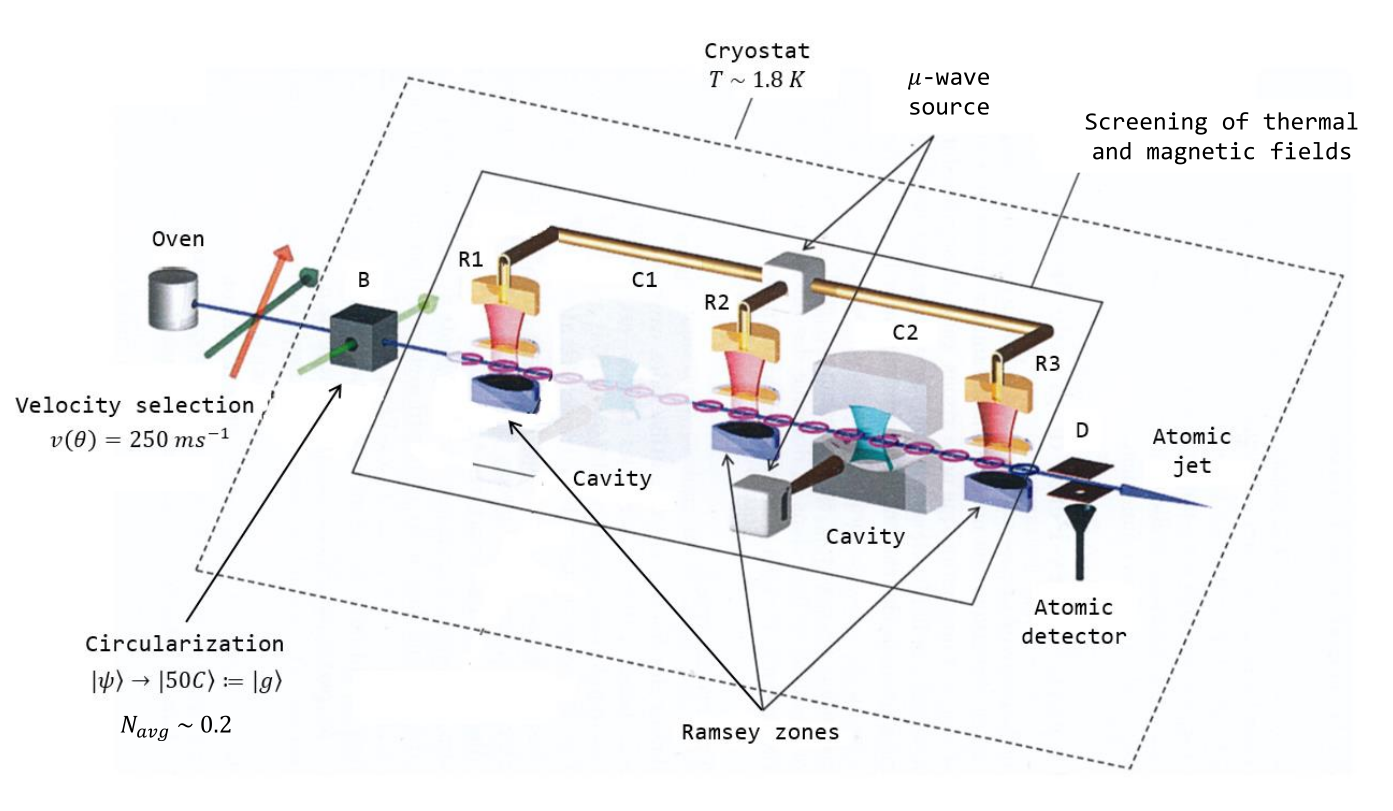
\includegraphics[width=\textwidth]{exp.png}
  \caption{A symbolic representation of the experiment (Credit: Luis Najera).
    The atoms leave from the oven, then they pass through a velocity selection
    mechanism that ensure that only atoms moving at the target speed are selected.
    Then, there is a circularization procedure that put all atoms in the state
    $\ket g$ that will be explained in \cref{ssec:atoms}. On average $0.2$ atoms
    go through in each batch. Most unselected atoms
    will still go trough the experiment but as they are not Rydberg atoms, they
    will not interact with anything including the detector. The three Ramsey
    zones are areas where we manipulate the atomic state through a classical
    micro-wave field. In the cavity C2 (C1 is unused), a certain state of the
    electromagnetic field is trapped with sufficiently few photons to observe
    quantum effects in its interaction with the atom going through.
    At the exit, atoms are detected by a projective measurement
    that give the energy level of the atom.}
  \label{fig:exp}
\end{figure}


\subsection{Circular Rydberg atoms}\label{ssec:atoms}

% From Section 3.3.1 of~\cite{Har06} and I.2.1.a of~\cite{SayPHD11}

The atoms are prepared in a specific circular Rydberg state called ``ground'' state
$\ket g$. It corresponds to the energy level $n = 50$. We will also use $\ket e$
called ``excited'' state which is the circular state at $n = 51$ and $\ket f$, the
``fundamental'' state with $n = 49$. Ideally, the atom should never get
in any other state during our protocol.
The gap between $\ket e$ and $\ket g$ is
approximately $\SI{51}{GHz}$, whereas the gap between $\ket g$ and $\ket f$ is
around $\SI{54}{GHz}$. These are microwave frequencies.

In most of our calculation we will manipulate our states by pairs, and not as the
whole triplet, because the atom will only interact with our setup at, or near,
a resonance frequency. We'll use the base $(\ket e, \ket g)$ in that order, but
the same is true for $(\ket g, \ket f)$. In such case, the Hamiltonian we will
use is
\[H = \frac {\hbar \omega}2 \sigma_Z,\]
 where $\omega$ is the gap frequency and $\sigma_Z$ in one of the
 three Pauli matrices used to describe a two-level system:
\[\twoline \sigma_Z = \mat{1&0\\0&-1} \gap \sigma_X = \mat{0&1\\1&0} \gap
  \sigma_Y = \mat{0&-i\\i&0}\]

It is important to note that the $X,Y,Z$ axis here have nothing to do with the
real world spatial axis. This is just a convention due to the fact that
this two-level system behaves similarly to a spin-1/2 system whose axis do have
spatial orientation.

From these operators we may also build the raising and lowering operators:
\[\sigma_+ = \frac{\sigma_X + i \sigma_Y}2 = \ket e \bra g = \mat{0&1\\0&0}
  \gap
  \sigma_- = \frac{\sigma_X - i \sigma_Y}2 = \ket g \bra e= \mat{0&0\\1&0}\]
They are equivalent to the annihilation and creation operators of a usual
harmonic oscillator (that I will present in \cref{ssec:rescav}). We can even
express the Hamiltonian in a similar way: $H = \hbar \omega(\sigma_+\sigma_- -
\frac12)$.





\subsection{Ramsey zone: Interaction with classical field}\label{sec:ramsey}

% From 3.3.2 of~\cite{Har06} and I.2.1.b of~\cite{SayPHD11}

In what we call Ramsey zone, the atom will be submitted to a classical oscillating
field at pulsation $\omega_f$, resonant (or near the resonance) with the atomic
transition. The field at the position of the atom will
be denoted by
\[\bs E = 2\mathcal{E}
  \mat{u_x\cos(\omega_f t + \varphi + \varphi_x)\\
    u_y\cos(\omega_f t + \varphi + \varphi_y)\\
    u_z\cos(\omega_f t + \varphi + \varphi_z)}\]
where $u_x^2 + u_y^2 +u_z^2 = 1$. We do not merge the global phase $\varphi$ into
the component phase to be able to use it later. This can be represented more
cleanly using $\bs u_f = \big(u_x e^{-i\varphi_x},u_y e^{-i\varphi_y},u_z
e^{-i\varphi_z}\big)$:
\begin{equation}\label{eqn:field}
\bs E = \mathcal{E} (\bs u_f\, e^{-i\omega_f t-\varphi} + \bs u_f^*\,
  e^{+i\omega_f t + \varphi}).
\end{equation}


With that field we can now express the Hamiltonian $H_f$ of the
interaction between the electric dipole of the
atom and the electric field. It is $H_f = - \bs D \cdot \bs E$ as proven in
section 3.1.2 of~\cite{Har06}.
The dipole operator can written in function
of the position operator $\bs R$ of the electron relative to the nucleus.
The exact expression is $\bs D = q \bs R$.
In our circular states having cylindrical symmetry,
we have $\bra e \bs R \ket e = 0$ and $\bra g \bs R \ket g = 0$,
so we only care about the off-diagonal terms. We write the dipole
operator as
\begin{equation}\label{eqn:D}
  \bs D = d\mat{\bs 0&\bs u_a^*\\\bs u_a&\bs 0} = d(\bs u_a \sigma_- + \bs u_a^* \sigma_+),
\end{equation}
such that $\bs u_a$ has unit length and expresses the direction
and $d$ is the value of the electric dipole
moment. They are defined by $ q \bra g \bs R \ket e = d \bs u_a$. The field
Hamiltonian has now the expression:
\[ H_f = -d\mathcal{E} \mat{\bs 0 &
  \bs u_a^* \cdot (\bs u_f\, e^{-i\omega_f t-\varphi} + \bs u_f^*\,
  e^{i\omega_f t + \varphi})\\
\bs u_a \cdot (\bs u_f\, e^{-i\omega_f t-\varphi} + \bs u_f^*\,
  e^{i\omega_f t + \varphi}) & \bs 0
}\]

The free Hamiltonian of the system being $H_a = \frac{\hbar \omega_a}2 \sigma_Z$,
we'll need to express the evolution of the system by separating both evolutions.
We will place ourselves in the interaction picture (explanation
in~\cref{app:pict}). Both the free and interaction Hamiltonians make the state turn
around, and we want to see the difference between the two of them. Therefore, we
remove $H_0 = \frac{\hbar \omega_f}2 \sigma_Z$. We remove the Hamiltonian
with the frequency of the field and not of the atom to simplify the field
frequencies elsewhere. The frequency of the atom in this new frame will be
$\Delta_r = \omega_a - \omega_f$.
Our new Hamiltonian $H_1 = e^{i\frac{H_0}\hbar t}(H_f + H_a - H_0)e^{-i\frac{H_0}\hbar t}$ is thus
\[H_1 = \frac{\hbar \Delta_r}2 \sigma_Z -
  d\mathcal{E} \mat{\bs 0 &
    \bs u_a^* \cdot (\bs u_f\, e^{-i\omega_f t-\varphi} + \bs u_f^*\,
    e^{i\omega_f t + \varphi}) e^{i\omega_f t}\\
    \bs u_a \cdot (\bs u_f\, e^{-i\omega_f t-\varphi} + \bs u_f^*\,
    e^{i\omega_f t + \varphi}) e^{-i\omega_f t} & \bs 0
  }\]

The two terms oscillating at frequency $2\omega_f$ are too fast to have
lasting effects, so we can neglect them: this is called the secular approximation.
The new Hamiltonian is thus
\begin{equation}\label{eqn:RamseyH}
H_1 = \frac{\hbar \Delta_r}2 \sigma_Z -\hbar \frac{\Omega_r}2
  \big(e^{-i\varphi}\sigma_+ + e^{i\varphi}\sigma_-\big),
\end{equation}
where $\Omega_r=\frac{2d}{\hbar}\mathcal{E}\bs u_a^* \cdot \bs u_f = \frac{2d}{\hbar}\mathcal{E}\braket{\bs u_a}{\bs u_f}$. We can put
some of $\varphi$ in $\bs u_f$ in \cref{eqn:field} to make $\Omega_r$ real
positive. Thus, the phase $\varphi$ is specific to the phase difference between the atom
and the field. It can be tuned by changing the phase of the field that we control.

When using the vector operator $\bs \sigma = (\sigma_X,\sigma_Y,\sigma_Z)$, our
Hamiltonian can be written as
\begin{equation}\label{eqn:rabi}
H_1 = \hbar \frac{\Omega_r'}2 \bs \sigma \cdot \bs n,
\end{equation}
where
\[ \Omega_r' = \sqrt{\Delta_r^2 + \Omega_r^2} \hspace {1cm}
  \text{and}\hspace{1cm} \bs n = \frac 1 {\Omega'_r}(-\Omega_r \cos \varphi,\;
  -\Omega_r \sin \varphi,\; \Delta_r).\]

One can show that $H_1$ represents a precession of the state of the atom on the
Bloch sphere around $\bs n$ at frequency $\Omega_r'$. This precession is named
``Rabi oscillation''. and is
represented on the Bloch sphere in \cref{fig:rabi}.
The pulsation $\Omega_r$ which is the frequency of
precession when the the frequencies match is named ``Rabi frequency''
\begin{figure}
  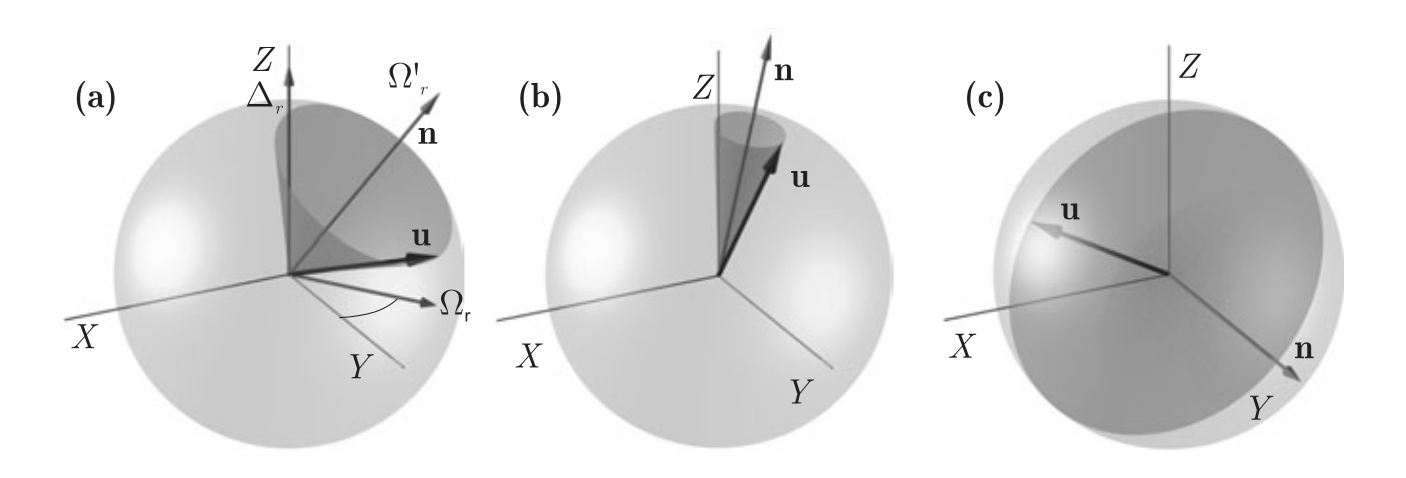
\includegraphics[width=\textwidth]{Rabi.png}
  \caption{
    Precession of the state $\bs u$ on the Bloch sphere. (a) When
    $\Omega_r$ and $\Delta_r$ are of same magnitude. The angle at which
    $\Omega_r$ is placed is $\varphi$. (b) When $\Delta_r$ is large :
    dispersive case. (c) When $\Delta_r =0$: full resonance case ($\varphi
    = 0$).
}
  \label{fig:rabi}
\end{figure}

By controlling the relative phase between the field and the atom as well as the
interaction duration (the vector rotates by an angle $\Omega'_r\Delta t$), we
can realize all possible rotations i.e nearly all unitary operation on this
two-level system. In practice, both parameters need to be carefully calibrated
because they can have huge effects with very small variations.

\subsection{Resonant cavities}\label{ssec:rescav}

% Harmonic oscillator: 3.1.1 of~\cite{Har06} and I.1.2.a of~\cite{SayPHD11}

A field mode in a cavity of a specific frequency $\omega_c$ can be modeled
as a usual one-dimensional harmonic oscillator. Its Hilbert space is
$\mathcal{H}_C = \C^\N$.
The basis of this space is composed of vectors $\{\ket n\}$, called \emph{Fock states}, with $n$ non-negative integer. One of the important operators in this space is the
number operator $N = \sum_n n\ket n \bra n$. The state $\ket n$ represents a
state with exactly $n$ photons. There are also the annihilation $a$ and creation $a^\dagger$ operators:
\[a = \sum_n \sqrt{n} \ket {n-1} \bra{n}.\]
Therefore, $N = a^\dagger a$ and the energy of the cavity is then
\[H_c = \hbar \omega_c \big(N + \tfrac 12\big).\]

We need to find how to represent a field oscillating at frequency $\omega_c$.
A general formula for a specific mode of the classical field is
\[\bs e(r) = \mathcal{E}\big(\bs f(\bs r) \alpha e^{i\omega_c t} + \bs f^*(\bs r)
  \alpha^* e^{-\omega_c t}\big),\]
where $\mathcal{E}$ is a general normalisation factor in units of $\SI{}{V/m}$, that
we'll compute later. A polarization function  $\bs f$
describes the spacial distribution of the electric field inside the cavity which
depends on the cavity shape.
We normalize it to $\|\bs f\|_\infty = 1$. Finally, $\alpha$ is the complex amplitude
of the field.

We know that on classical harmonic oscillatiors, the eigenvectors of $a$, named
\emph{coherent state} represent directly classical states. I remind that for
each complex number $\alpha \in \C$, there is a unique state (up to phase shift)
$\ket \alpha$ such that $a \ket \alpha = \alpha \ket \alpha$.
Let's prove that in the case of field mode oscillator, the coherent state also
represents a classical state.

\begin{prop}
  A coherent state $\ket{\phi(0)} = \ket \alpha$ evolves as:
  \[ \ket {\phi(t)} = \ket {\alpha e^{i\omega_c t}} \]
\end{prop}

\begin{proof}
  In the section \emph{time evolution} of the section 3.1.2 of \cite{Har06}
\end{proof}

Therefore, we define the electric field operator to be
\begin{equation}\label{eqn:Eop}
\bs E(\bs r) = \mathcal{E}\big(\bs f(\bs r) a + \bs f^*(\bs r)
  a^\dagger \big).
\end{equation}
It will behave exactly as a classical field for coherent state and be a
superposition of classical field for other states. We can determine the value of
$\mathcal{E}$ from the field energy operator:
\[ H = \int \varepsilon_0 |{\bs E}|^2 \dd^3 \bs r \]

\begin{prop}
  The value we get for $\mathcal{E}$ is
\[ \mathcal{E} = \sqrt{\frac{\hbar \omega_c}{2 \varepsilon_0 \mathcal{V}}}\]
where $\mathcal{V} = \int \bs |f(\bs r)|^2\dd^3\bs r$ is the effective mode volume
\end{prop}

\begin{proof}
  Just do $\bra n H \ket n = \bra n \int \varepsilon_0 |{\bs E}|^2 \dd^3 \bs r
  \ket n$ and expand everything.
\end{proof}

The value $\mathcal{E}$ is some kind of the average (more like r.m.s) field per
photon in the cavity.

\subsection{Atom-cavity interaction}\label{sec:atomcav}

% From 3.4 of~\cite{Har06} and I.3 of~\cite{SayPHD11}

In this section we'll see what happens when we put a two-level atomic system in
a cavity at or near resonance frequencies. The systems are then coupled during
all interaction time, in particular the states $\ket{g,n+1}$ and $\ket{e,n}$,
blend together as if absorbing and emitting photons continuously. The model we
use is called the James-Cumming model.

\subsubsection{General case}

In the general case, we just reuse the dipolar approximation Hamiltonian for the
interaction:
\[H_i = - \bs D \cdot \bs E\]
By using \cref{eqn:D} and \cref{eqn:Eop}, and assuming that the atom is at
position $\bs r$, we get :
\[H_i = - d(\bs u_a \sigma_- + \bs u_a^* \sigma_+) \cdot \mathcal{E}\big(\bs
  f(\bs r) a - \bs f^*(\bs r)
  a^\dagger \big).
  \]


For sake of simplification, we assume the atom is more or less in the middle
of the cavity and thus that $\bs f(r) = \bs u_c$ of unit length.
If we do the same Heisenberg picture as in \cref{sec:ramsey}, we'll see that
terms associated with pure energy gain ($\sigma_+a^\dagger$) or loss ($\sigma_-a$)
oscillates very quickly at the order of $2\omega_c$,
whereas the one corresponding to photon absorbtion ($\sigma_+a$) or emission
($\sigma_-a^\dagger$) oscillates at a more reasonable frequency. We can
thus do the secular approximation again to obtain:
\begin{equation}
  H_i = \frac{\hbar \Omega_0}2 (\sigma_+a + \sigma_-a^\dagger),
\end{equation}
where the \emph{vacuum Rabi frequency} reads:
\[\Omega_0 = -2\frac {\mathcal{E}d \braket{\bs u_a}{\bs u_c}}{\hbar}.\]

Here again, for the sake of simplification, the cavity field and the atom are
considered to be in phase, and thus $\braket{\bs u_a}{\bs u_c}$ is real
negative so that $\Omega_0 > 0$. The full Hamiltonian is then
\begin{equation}
H_{ac} = \frac{\hbar \omega_a}2 \sigma_Z + \hbar \omega_c \big(N +
  \tfrac12\big) + \frac{\hbar \Omega_0}2 (\sigma_+a + \sigma_-a^\dagger).
\end{equation}

With this Hamiltonian, the states $\ket{e,n}$ and $\ket{g,n+1}$ are coupled 2 by
2, except for $\ket{g,0}$ which is stationary. On the space $\mathcal{S}_n =
\Span(\ket{e,n},\ket{g,n+1})$, the Hamiltonian is
\[\twoline H_n = \hbar \mat{\omega_c(n+1) + \frac{\delta}2& \frac{\Omega_n}2\\
    \frac{\Omega_n}2&\omega_c(n+1) - \frac{\delta}2}\]
with $\Omega_n = \sqrt{n+1} \,\Omega_0$. Its eigenvectors are given by
\newcommand{\tnt}{\frac{\theta_n}2}
\begin{align*}
  \ket{+,n} &= \cos \tnt \,\ket{e,n} + \sin \tnt \ket{g,n+1}\\
  \ket{-,n} &= \sin \tnt \,\ket{e,n} - \cos \tnt \ket{g,n+1}\\
\end{align*}

\vspace{-0.5cm}

with $\theta_n \in [0,\pi]$ and $\tan \theta_n = \frac {\Omega_n}{\delta}$.
These states are called \emph{dressed states}.
We can define again $\Omega'_n = \sqrt{\Omega_n^2 + \delta^2}$ to have the energies

\vspace{-0.2cm}

\[E_{\pm,n} = \hbar \omega_c(n+1) \pm \frac{\hbar \Omega_n'}2.\]

\vspace{0.2cm}

\begin{figure}
  \centering
  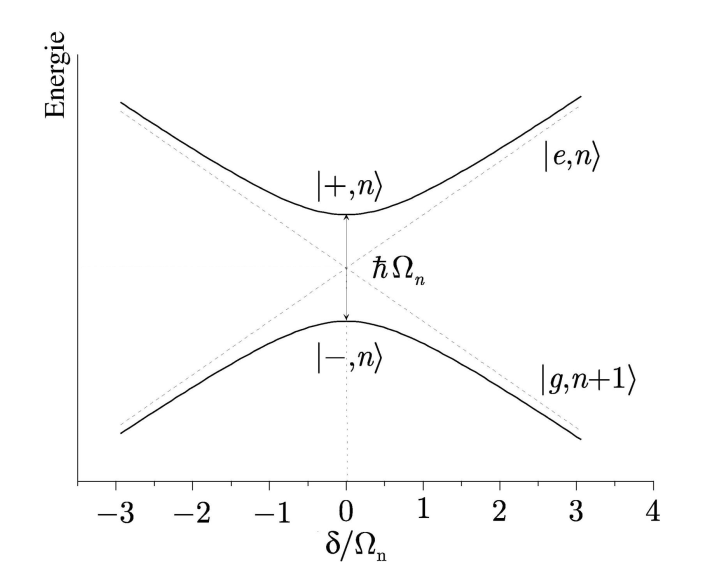
\includegraphics[scale=0.3]{dressed.png}
  \caption{The energy of dressed states at level $n$ as a function of the atom-cavity detuning $\delta$ (in units of $/\Omega_n$).}
  \label{fig:dressedenergy}
\end{figure}

Those energies are represented in \cref{fig:dressedenergy}.



\subsubsection{Effective interaction time}
\newcommand{\eff}{_{e\!f\!\!f}}

Let's go back to the hypothesis that $\bs f(\bs r)$ is of unit length. According
to~\cite{SayPHD11}, it is proven in~\cite{Har06} that, if the atom crosses the
cavity horizontally, instead of actually caring about the exact form of the
field, we can assume that everything behave like the atom traversed a full blown
field with $\|\bs f(\bs r)\| = 1$ that has an effective width $w\eff$. For an
atom at speed $v$, all happens as if it is submitted to the Hamiltonian $H_{ac}$
during
\[t\eff = \frac{w\eff}v.\]

\subsubsection{Resonant case}

If $\delta = 0$, the Hamiltonian is of the form $H = \hbar \omega_c(n+1) + H_1$
where $H_1$ is the Rabi Hamiltonian in \cref{eqn:rabi} and $\bs n =
\bs u_x$. Therefore each pair of states at level $n$ will oscillate around $\bs
u_X$ at pulsation $\Omega_n$. In particular if the cavity is empty and the atom
arrives in state $\ket e$, the atom will absorb and emit a photon at pulsation
$\Omega_0$ which is thus the \emph{Vacuum Rabi pulsation}.

\subsubsection{Dispersive case}\label{sssec:disp}

In the dispersive case i.e far off the resonance point we have a completely
different behaviour. The energy the atom cannot really change because, the
energy of the photons do not match the interstate gap. However, if we do a
pertubative analysis in $\delta \gg \Omega_n$, we get some more usable results.
For simplicity, we assume that $\delta > 0$.

In this analysis the new energies are
\[E_{\pm,n} = \hbar \omega_c(n+1) \pm \frac{\hbar }2 \left(\delta + \frac{\Omega_n^2}{2\delta}\right),\]
but the in this situation we have:
\[ \ket{+,n} \approx \ket{e,n} \gap \text{and}\gap \ket{-,n} \approx \ket{g,n+1} \]

If $E_{e,n} = \hbar \omega_c(n + \frac12) + \frac\hbar2\omega_a$ is the normal
energy of state $\ket{e,n}$, the new one will be
\[E_{+,n} = E_{e,n} + \frac{\Omega_0^2}{4\delta}\left(n + 1\right).\]
and similarly for the other case:
\[E_{-,n} = E_{g,n+1} - \frac{\Omega_0^2}{4\delta}\left(n + 1\right)\]



If the cavity is in state $\ket n$, The sum of the difference in pulsation of
$\ket{e,n}$ and $\ket{g,n}$ is thus:
\[\Delta\omega_a = \frac{\Omega_0^2}{2\delta}\left(n + \frac 12\right)\]

Up to a global shift, all happens as if for an effective interaction time $t\eff$,
we have a shift of phase $\phi_0 = \frac{\Omega_0^2}{2\delta}t\eff$ per photon.
It is important to note that the most controllable parameter here is $\delta$ via the stark effect
on the atom.


% \section{Experimental details and calibration}


% This section was supposed to explain some part of the little experimental details that I've seen
% or interacted with. I'll try to write it by Monday night. Otherwise, most of the
% details can be found in~\cite{SayPHD11}.
% There is also a bunch of thing I don't know as this
% experiment is the work of several year of research. It can be skipped for a
% first reading as the details are not essential to understand the rest of this report.


% \subsection{Atomic State preparation}

% I.2.3.b


% % oven
% % speed filtering Laser with doppler + resonnance
% % State filtering (n=52)
% % We ignore non-Rydeberg atoms

% \subsection{Cavity state preparation}

% Stuff about coherent state in 3.1.3?

% The right stuff is probably in 3.2

% I.1.2.b

% \subsection{State stability}\label{ssec:ststab}

% I.2.3.a

% \subsection{Stark shift}

% I.2.3.a?

% \subsection{Detection of atom}

% I.2.3.d

% % see thesis for functioning of detector

% \subsection{Cooling and relaxation times}

% I.1.2.b

% % Say some stuff about cooling

\section{QND Measurement}

Quantum Non-Destructive measurement(QND) is a kind of quantum measurement that tries
to preserve the state of the observed system. By having the observed system
interacting weakly with other systems, we can sometimes gather enough
information to reconstruct the state.

The QND measurement in the current experiment is realized by sending a sequence
of individual atoms prepared in a superposition state $\ket{g}+\ket{e}$ through
the
cavity and interacting with it dispersively. One can see in~\cref{sssec:disp} that
an atom in this case will undergo a phase shift between its states
proportional to the number of photons stored in the cavity field. If we
calibrate our system to have an interesting $\phi_0$, the atomic states will be
dispersed accordingly on the equator of the Bloch sphere depending on the number
of photons
in the cavity. We can then do a $\frac\pi2$ Rabi-pulse at a specific phase to
rotate the equator to a polar circle on the Bloch sphere. Then, when we measure the
atom, the probabilities of being observed in $\ket e$ or $\ket g$ depends on the
number of photons in the cavity. This setup is called a Ramsey interferometer.
By varying the phase of the last Rabi pulse we can gather enough statistical
information to recreate the state of the cavity.

However the only concrete output we get is a long list of state detections in
$\ket e$ and
$\ket g$, so we need a statistical tool to reconstruct a corresponding
density matrix from this data.


\chapter{Maximum likelihood reconstruction}

I put some reminders about multivariate covariances in
\cref{app:cov}, which could be useful in this chapter.

\section{Basics of the estimation theory}

\subsection{Estimator}

The goal of estimation is to estimate some parameters using observations or
measurements. In the simplest case, we measure a random output $X \in \mathcal{X}$ from an
unknown input $\theta \in \Theta$. We place ourselves in a model where the law
of $X$ conditionally to $\theta$ is known. Formally, we have for each $\theta$ a
probability measure $P_\theta$ on $\mathcal{X}$. If $P_\theta$ has the right
form (in particular, if $X$ is a vector of repetition of the same experiment), we
can extract information on $\theta$ from $X$. For that we can use an estimator.

\begin{defn}
  An \emph{estimator} of parameter $\theta$ from $X$ is just a deterministic
  function $\hat \theta(X)$ that provides the most likely value of $\theta$ that
  could have resulted in $X$.
\end{defn}

\begin{rem}
  The estimator notation $\hat \theta$ has noting to do with the notation of
  quantum operator in quantum mechanics. It should usually be clear from the
  context which one it is.
\end{rem}

\

The most frequent case of parameter is $\theta \in \R$. In that case we can
easily compare the original $\theta$ with its estimator $\hat \theta$ with a
subtraction:

\begin{defn}
  For a given $\theta$, the \emph{bias} of the estimator $\hat \theta$ is
  \[B(\hat{\theta}) = E_\theta(\hat{\theta}(X) - \theta),\]
  where the expectation $E_\theta$ is taken on the law $P_\theta$. An estimator
  is \emph{biased} if the bias is non zero and it is \emph{unbiased} otherwise.
\end{defn}

\begin{defn}
  For a given $\theta$, the \emph{variance} of the estimator $\hat \theta$ is
  \[V(\hat{\theta}) = E_\theta\Big({(\hat{\theta}(X) - \theta)}^2\Big).\]
\end{defn}

\subsection{Likelihood}

In the case where all probability measures $P_\theta$ are absolutely
continuous against a ``canonincal'' measure $\mu$ on $\mathcal{X}$, we can
define a function $f(x;\theta)$ such that
\[P_\theta(A) = \int_A f(x;\theta)\,\dd \mu(x).\]

\begin{defn}
  For a given observation $x \in \mathcal{X}$, we define the \emph{likelihood} function
  $\mathcal{L}_x(\theta) = f(x;\theta)$.
\end{defn}

\begin{defn}
  For a given observation $x \in \mathcal{X}$, we define the \emph{log-likelihood} function
  $\ell_x(\theta) = \ln \mathcal{L}_x(\theta)$.
\end{defn}

\subsection{Fischer information and Cramér-Rao bound}

We now assume a set of real parameter $\theta \in \mathcal{D} \subset \R^n$.
A way to know if we could improve our estimation at a specific point is the
gradient of the log-likelihood function. This is called the
\emph{score}. We have $s_x(\theta) = \partial_\theta \ell_x(\theta)$. The
lower the score (its norm, actually), the better our estimation.

\begin{prop} The expectation of the score is 0.
\end{prop}
% \begin{proof}
%   Left to the reader.
% \end{proof}

We can then study the variance of score and its covariances with other things.
In particular:

\begin{lem}\label{lem:corscr}
  The covariance of the score and any unbiased estimator is the identity:
  \[\cov(\hat \theta, s_x(\theta)) = I\]
\end{lem}

% \begin{proof}
%   Left to the reader.
% \end{proof}

In the light of the theorem about bounds of \cref{sec:correl}, we can give special
interest to the variance of the score and its link with the variance of any estimator.

\begin{defn} The \emph{Fischer information} of the parameter $\theta$ is defined
  as the variance of the score:
  \[I(\theta) = V\big(s(\theta)\big).\]
\end{defn}

If $\theta \in \R$, this is just the expectation of the square of the score, but
otherwise, $I(\theta)$ is a covariance matrix thus at least positive
semi-definite.
This information value puts a bound on the minimum variance of any
unbiased estimator, which is called the Cramér–Rao bound.

\begin{thm}[Cramér–Rao bound]
  For any unbiased estimator $\hat \theta$ and if $I(\theta) > 0$, we have
  \[V(\hat{\theta}) \ge {I(\theta)}^{-1}.\]
\end{thm}

\begin{rem}
  In the multivariate case, the ${}^{-1}$ obviously means the inverse of the matrix
\end{rem}

\begin{proof}
  The bound on multivariate correlation is proven in \cref{thm:correln}. The
  bound is written as
  \[\cov(X,Y){V(Y)}^{-1}\cov(Y,X) \leq V(X).\]

Since $I(\theta) = V(s_x(\theta))$ and from \cref{lem:corscr}, the bound holds.
\end{proof}

In order to have a better interpretation of the Fischer information, if the
likelihood is at least $\class 2$ in $\theta$, we can rewrite
it as a hessian:

\begin{prop}\label{prop:fisherhessian}
  Under sufficient regularity assumption,
  the Fischer information can also be written as the opposite of the Hessian of the
  log-likelihood function:
  \[I(\theta) = -\frac{\partial^2 \ell}{\partial \theta^2}(\theta).\]
\end{prop}

% \begin{proof}
%   Left to the reader.
% \end{proof}







\section{Maximum likelihood estimator}

\subsection{Definition}

Now that we have proven the best variance possible, we still have to build an
estimator approaching this bound. There are many different kinds of estimator. The
most used one is the average when $X = (X_1,\ldots,X_n)$ and
$E_\theta(X_i) = \theta$ and $V_\theta(X_i)$ is small enough. However, in more
complex cases this won't work. The goal of the estimator is to produce the more
likely $\theta$, ideally the maximum of a density function $p(\theta | X)$.

If all measures can be expressed as density functions, using Bayes law, we obtain
\begin{equation}\label{eqn:bayes}
  p(\theta|x) = p_\theta(x) \frac {p(\theta)}{p(x)}
  = p_\theta(x) \frac {p(\theta)}{\int p_{\theta'}(x)p(\theta')\,\dd \theta'}.
\end{equation}

We aim now to maximize $p(\theta|x)$. However, that
formula only makes sense if we have a prior law on $\theta$. If the prior
distribution is more or less uniform, it is the same as maximizing $p_\theta(x)
= \mathcal{L}_x(\theta)$.

\begin{defn}
  The \emph{maximum likelihood estimator} $\theta\ml$ is defined by:
  \[\theta\ml(x) = \argmax \mathcal{L}_x.\]
\end{defn}

The maximum likelihood have no excessively nice properties in its own. But
when $X = (X_1,\ldots,X_n)$, where all the $X_i$ come from the same law
$P_\theta(X_0)$ and are independent, and if $n \to \infty$,
it has nice convergence properties. In particular, it will converge in
probability to the right
$\theta$ and saturate the Cramér-Rao bound as $n \to \infty$.
\

In practice, as most probability laws are log-concave (in particular the normal
law), we use the log-likelihood, $\ell_x$ instead of $\mathcal{L}_x$. Apart
from concavity, this also has the advantage that multiple repetition are
additive instead of multiplicative:
\[\mathcal{L}_x(\theta) = \prod_i \mathcal{L}_{x_i}(\theta) \quad \quad \quad
  \quad \ell_x(\theta) = \sum_i \ell_{x_i}(\theta).\]
In particular, the probability goes down to zero very quickly. Computing it on
a 64-bit machine floating point numbers, there is a high risk of $\mathcal{L}$ to
be simply evaluated to zero when it is just really small. Noye yjay natural logarithm of the minimum positive 64-bit floating point number
is $-740$.

% \subsection{Informal properties}

% I do not remember exactly what I wanted to put here this will probably get deleted.

% Put the probability function according to Vincent's thesis.

% Add the case at the edge of $\mathcal{D}$.

\chapter{Computation of effect matrices }

In this chapter, we stay in Hilbert spaces of finite dimension. Most of the
result can be extended to Hilbert spaces of countable dimension by adding
some restriction.
Since we won't need them in the rest of the report, I won't mention infinite
dimension anymore. The space of operator on
$\mathcal{H}$ is denoted by $\mathcal{L}(\mathcal{H})$. The set of observables
(Hermitian operators) is denoted by $\mathcal{O}(\mathcal{H})$. The set of
unitary operators on $\mathcal{H}$ is denoted by $\mathcal{U}(\mathcal{H})$.

\section{Density matrices}

\subsection{Justification}

In order to make significant observation with an imperfect experimental setup, we need to make averages and statistics on quantum state.
One way of doing that would be to manipulate probability measure over state
space which is the unit sphere $S$ of the model Hilbert space $\mathcal{H}$. However, if we look at
it in details, there are a lot of distributions that are indistinguishable by any
measurement. In the first approximation, we say that two probability distribution
$\lambda$ and $\mu$ on $S$ are indistinguishable,
if for any observable $A$ (Hermitian matrix) on $\mathcal{H}$, we
have
\[\int_S \bra \phi A \ket \phi\,\dd \lambda(\phi) = \int_S \bra \phi A \ket
  \phi\,\dd \mu(\phi) .\]

However, if we rewrite it, we obtain
\[\int_S \bra \phi A \ket \phi\,\dd \lambda(\phi)
  = \int_S \Tr\big(\ket \phi \bra \phi A\big) \,\dd \lambda(\phi)
  = \Tr\left(\int_S \ket \phi \bra \phi \,\dd \lambda(\phi) A \right).\]

\begin{defn} We define the density matrix of a probability distribution $\lambda$ on
  quantum states:
  \[ \rho = \int_S \ket \phi \bra \phi \,\dd\lambda(\phi) .\]
\end{defn}
\begin{prop}
  The average of an observable $A$ in any probability distribution $\lambda$ is
  given by $\Tr(\rho A)$.
\end{prop}

\begin{rem} This is sufficient to fully characterise the distribution, because
 any observable $A$ can be written as $A = \sum_a aP_a$, where $P_a$ are orthogonal
 projector and are also observables. The average of $P_a$ is $\Tr(\rho P_a)$ and
 thus for all distributions having density matrix $\rho$, the probability
 of output $a$ when measuring $A$ is the same.
\end{rem}

Since two distribution that share the same
density matrix are completely indistinguishable by any measurement, in the rest of this report, we will use density matrix as the only
representation of quantum distribution. In practice,
as quantum physicist manly manipulate probabilistic quantum state and not that
much usual \emph{ket} state, the term quantum state is used for a statistical
mixture described by a density matrix. A state of the form $\ket \phi$ is thus
called a \emph{pure} state.

\subsection{Properties}

We can now study what are density matrices and find necessary and sufficient
conditions for a matrix to be a density matrix.

\begin{prop}\label{prop:dens}
  A density matrix is Hermitian positive ($\rho > 0$) of trace 1.
\end{prop}

\begin{proof}
  $\ket \phi \bra \phi > 0$, so $ \int_S \ket \phi \bra \phi \,\dd\lambda(\phi)
  > 0$.
  $\Tr(\ket \phi \bra \phi) = 1$, so $\Tr(\rho) = \lambda(S) = 1$.
\end{proof}

If we want to prove that is sufficient we need to look at the spectral
decomposition.
In finite dimension $n$, a spectral decomposition of $\rho$ give a
collection of eigen values $p_1, \ldots, p_n$ which sum up to~1. They are the
analogous of probabilities in classical probability theory. The density matrix
can then be written as
\[\rho = \sum p_i \ket {\phi_i} \bra {\phi_i}.\]

\begin{thm} The condition~\ref{prop:dens} is necessary and sufficient i.e any Hermitian positive matrix of trace 1 is a density matrix.
\end{thm}

\begin{proof}
  Any matrix satisfying the condition~\ref{prop:dens} can be decomposed in
  $\rho = \sum p_i \ket {\phi_i} \bra {\phi_i}$, and thus the atomic measure
  $\lambda(\{\ket {\phi_i}\}) = p_i$ give exactly that density matrix.
\end{proof}

The set of density matrix will be denoted by $\mathcal{D}(\mathcal{H})$ (or just
$\mathcal{D}$ when there is no ambiguity). We have the inclusions:
\[\mathcal{D}(\mathcal{H}) \subset \mathcal{O}(\mathcal{H}) \subset \mathcal{L}(\mathcal{H}).\]

As a density matrix is an observable, we can study its behavior as an observable.
In state $\ket \Psi$, the average $\langle \rho \rangle$ is the probability of
state $\ket \Psi$ if we did a projective measurement in an orthonormal base that
contains $\ket \Psi$. $\rho$ is thus like an observable of classical probability.

\subsection{Rank and purity}

In finite dimension, we can also look at the
rank of the density matrix that gives a lot of information.

\begin{prop}
  The rank of the density matrix $\rho$ is the dimension of the support of any
  probability distribution that can give this matrix
  (with the convention $\dim A = \dim \Span(A)$).
\end{prop}

\begin{defn}
  If a density matrix $\rho$ has rank one, it only represents one unique state and can be written
  $\rho = \ket \phi \bra \phi$. It is thus called a \emph{pure state}. No
  difference is made between the state $\ket \phi$ and the density matrix $\ket
  \phi \bra \phi$ as both are called pure states.

  On the other hand if $\rk \rho > 1$, the density matrix represent a
  \emph{mixed state}: a statistical mixture of states.
\end{defn}

\begin{rem}
  It is very important to differentiate a quantum superposition for a
  statistical mixture. For example on a qubit,
  $\ket + = \frac1{\sqrt 2} \ket 0 + \frac1{\sqrt2} \ket 1$ is a quantum
  superposition while a statistical mixture would be
  $50$ \% of $\ket 0$ and $50$\% of $\ket 1$. When the state in measured in base
  $\ket0,\ket1$, the results will be the same but in an other basis they could be
  different. In particular, in basis $\{\ket +, \ket -\}$, the first state will be
  measured as $100$ \% $\ket +$ and $0$ \% $\ket -$, but the second will still be
  50\,--\,50 of $\ket+$ and $\ket -$.
\end{rem}

\begin{prop}
  A state $\rho$ is pure iff $\Tr \rho^2 = 1$.
\end{prop}

\begin{proof}
  $\Tr (\rho^2) = \sum p_i^2 < 1$ unless one $p_i$ is one and the others 0.
\end{proof}

The value $\Tr \rho^2$ has in fact much more interesting properties, and thus
deserves a name.

\begin{defn}
  The \emph{purity} of a quantum state represented by $\rho$ is defined as $\gamma = \Tr \rho^2$.
\end{defn}

\begin{prop}
  In dimension $d$, the purity is always between $\frac1d$ and $1$. If $\gamma =
  \frac1d$, then $\rho = I$, the represented mixture is uniform and we have
  absolutely no information on the state. If $\gamma = 1$, the state is pure and
  we thus have complete information on the quantum state.
\end{prop}

\begin{proof} $\Tr (\rho^2) = \sum p_i^2 \leq 1$.
  But the projection of $0$ on the hyper plane of sum $1$ is $\frac I d$ which
  has therefore the lowest norm of that plane which is $\frac I d$.
\end{proof}

The main interest of purity is that it remains constant during unitary evolution
($\Tr (U^\dagger \rho U) = \Tr \rho^2$),
whereas it will change in any other evolution (relaxation, decoherence,
measurement etc) as we lose or gain information.

\subsection{Matrix coefficients}

When we express the density matrix in a specific base, we gain a lot of
information on the state projected in that basis, in particular on how
projective measurements in that basis takes place.

\begin{defn}
  When $\rho$ is express in the basis $\ket 1, \ldots, \ket d$, the diagonal
  coefficients, which are real and non-negative, are called \emph{populations}. The
  coefficient $\bra i \rho \ket i$ equals the probability to obtain state $i$,
  when measuring $\rho$ in this basis.

  The non-diagonal coefficients are complex and called \emph{coherences}. The
  coherence between states $\ket i$ and $\ket j$ is $\bra i \rho \ket j$. It is conjugate to the coherence between $\ket j$ and $\ket i$.
\end{defn}

The point of this distinction is that any projective measurement made in that
basis will have the same statistics whatever the value of coherences. Their
values will only matter when measuring value in other bases or when the state
is evolving. This also means reciprocally, in the context of tomography,
that measurements made in that basis can bring no information.

As we will reconstruct $\rho$ numerically and will use this matrix
representation, we need to study the structure of $\mathcal{D}(\mathcal{H})$ in
this form. In particular:

\begin{prop}
  $\dim \mathcal{D}(\mathcal{H}) = d^2 - 1 $ as a real vector space.
\end{prop}

\begin{proof}
  The (real) dimension of $\mathcal{O}(\mathcal{H})$ is $d^2$ because there are $d$ diagonal
  coefficient and $\frac {d(d-1)} 2$ complex off-diagonal coefficient so $d +
  d(d-1)$ coefficients in total. The constraint $\Tr \rho = 1$ removes one degree
  of freedom, so we only have $d^2 -1$ dimensions.
\end{proof}

\subsection{The case of a qubit}

In the case of a qubit, with $\dim \mathcal{H} = 2$ (complex dimension), we know
that the pure states, up to a phase shift, can be represented on the Bloch sphere. We
would like to know how to represent mixed states. The dimension of
$\mathcal{D}(\mathcal{H})$ is 3, so we can hope for a simple representation. Any
density matrix from $\mathcal{H}$ can be written as
\[\rho = \frac12I + S,\]
where $\Tr S = 0$. A basis of the hyperplane of zero-trace hermitian matrice can
be given by Pauli matrices:
\[\sigma_Z = \mat{1&0\\0&1} \quad \quad \sigma_X = \mat{0&1\\1&0} \quad \quad
  \sigma_Y = \mat{0&-i\\i&0}.\]

If we write $\bs\sigma = (\sigma_X,\sigma_Y,\sigma_Z)$, we obtain
\[\rho = \frac12 I + \bs r \cdot \bs \sigma,\]
where $\bs r \in \R^3$ is a usual 3D vector. Furthermore, we have:

\begin{prop}
  $\rho \geq 0$ if and only if $\|\bs r\| \leq 1$.
\end{prop}

\begin{proof}
  $\det \rho = 1 - \|r\|^2$
\end{proof}

We can then look at the purity $\gamma$ in function of $\bs r$. We have:

\begin{prop}
  $\gamma = \Tr(\rho^2) = \frac 12 (1 + \|\bs r\|^2)$
\end{prop}

\begin{cor}
  $\rho$ is pure if and only if $\|\bs r\| = 1$
\end{cor}

Mixed states are thus represented by the Bloch ``ball''. The pure states are laying on its surface i.e.\ on the sphere. One can check that this representation matches the usual Block sphere representation of pure states. The
maximally miwed state $\frac I2$ is in the center of the ball.

\subsection{Composite systems and partial trace}

Next, we model a density matrix of a composite system. For a pure separable state,
this is a simple tensor product $\ket{\Psi\Phi} = \ket \Psi \otimes \ket \Phi =
\ket \Psi\ket\Phi$. Luckily for us we have
\[(\ket\Psi\ket\Phi) \otimes (\bra\Psi\bra\Phi) = \ket\Psi\bra\Psi \otimes \ket
  \Phi \bra \Phi,\]
where $\otimes$ designate the tensor product of operators and matrices.
We still have the same property of entanglement, i.e. the state is entangled iff
the density matrix cannot be written as a tensor product.

What is interesting now is to study the statistical result of measurement performed on one of the two quantum subsystems $\mathcal{H}_1$ and $\mathcal{H}_2$.
If we take an observable $A$ on $\mathcal{H}_1$ and its extension to
$\mathcal{H} = \mathcal{H}_1 \otimes \mathcal{H}_2$ which is $\tilde A = A
\otimes I$. If we have a density matrix $\rho = \rho_1 \otimes \rho_2$, then the
average of $A$ is $\Tr(\rho \tilde A) = \Tr(\rho_1A)\Tr(\rho_2) = \Tr(\rho_1A)$.
On a tensor product density matrix, the evaluation of $\tilde A$ only depends on
the part of $\rho$ in $\mathcal{H}_1$ and we would like to express that on any
density matrix. In order to do that, we rewrite our computation as
$\Tr(\rho\tilde A) = \Tr((\rho_1\Tr(\rho_2))A)$ and see that
$\rho_1\Tr(\rho_2)$ is the part of $\rho$ in $\mathcal{H}_1$.

\begin{defn}
  Given a tensor product $\mathcal{H} = \mathcal{H}_1 \otimes \mathcal{H}_2$,
  The \emph{partial trace over $\mathcal{H}_2$}, is a linear operator
  $\Tr_{\mathcal{H}_2} : \mathcal{L}(\mathcal{H}) \to
  \mathcal{L}(\mathcal{H}_1)$ defined on tensor product by
  \[\Tr_{\mathcal{H}_2}(\rho_1\otimes \rho_2) = \rho_1 \Tr(\rho_2)\]
  and extended by linearity on the full $\mathcal{L}(\mathcal{H})$.
\end{defn}

\begin{prop}
  For any operator $\rho \in \mathcal{L}(\mathcal{H})$, and any observable
  $A\in\mathcal{O}(\mathcal{H}_1)$, we have:
  \[\Tr(\rho(A \otimes I)) = \Tr(\Tr_{\mathcal{H}_2}(\rho)A)\]
\end{prop}

\begin{proof}
  It's true if $\rho$ is a tensor product and so it is true on any $\rho$ by linearity.
\end{proof}

An important remark to be made is that if a pure state in entangled, its partial
trace is mixed states. If we ignore the other space, our
space will behave as a statistical mixture and not as a quantum superposition
because depending of what the other state becomes, we can have any different phase.
For example if we have two qubits, and we have a
Bell state $\ket \psi = \frac{\ket{00} + \ket{11}}{\sqrt 2}$, then
\[\Tr_2\big(\ket \Psi \bra \Psi\big) = \frac 12I.\]


\section{Quantum operations}

Even if a closed quantum system follows a unitary evolution, quantum
systems are in general open. They undergo interaction with their environment, whether it is
from external measurement or simply thermal relaxation. The goal of this section
is to construct a representation of acceptable transformation for open systems similar to those describing unitary evolution of a closed system.
This section is strongly inspired from~\cite{QCQI}.

\subsection{Classical measurement}

The first and simplest example of external interaction in quantum theory is a
measurement. When a quantum system interacts with a macroscopic measurement
device, it is measured and collapsed in a specific state. The usual framework for
measurement is projective measurement. It is
made by measuring a observable that fully describes the measurement
process.

Let $A \in \mathcal{O}(\mathcal{H})$ be an observable on $\mathcal{H}$. The
spectral decomposition of $A$ tells us that $A = \sum_a a P_a$, where $a$
are eigenvalues of $A$ and $P_a$ are orthogonal projectors on the
corresponding eigenvector spaces. When starting in state $\ket \Psi$, we
measure $a$ with probability $\bra \Psi P_a \ket \Psi$ and we get
the output state
\[ \frac{P_a \ket \Psi}{\sqrt{\bra \Psi P_a \ket \Psi}}.\]

In fact, $P_a$ is also a quantum measurement operator which detects if we measure
$a$ or not, and thus its average value is the probability of measuring $A$. We
can then express the same thing in the space of density matrices. When starting in
$\rho$, we expect $a$ with probability $\Tr(\rho P_a)$ and get as an output
state
\[ \frac{P_a \rho P_a}{\Tr(\rho P_a)}.\]

An important question when dealing with probability is whether they always sum to
one, and in this case, this is answered by the closure relation
\[\sum_a P_a = I\]
and as $\bra \Psi I \ket \Psi = \Tr(\rho I) = 1$, the probabilities are normalized.

\subsection{Generalized measurement}

In some case quantum detector can perform other kinds of measurement, different from projective ones.
In particular, a measurement that completely destroys the object instead of
projecting is in a specific vector space. The main example is a photon counting
detector. When a cavity is in a Fock state $\ket n$, and we insert a photon
counting detector, the photons ``crash'' into the detector and are counted to be
$n$. The remaining state is always $\ket 0$, as there is no photon left. This
measurement is obviously non projective as $\ket 0$ is orthogonal to any $\ket
n$ with $n>0$. We thus need a framework to handle this kind of measurement.

While a projective measurement of operator $N$, would have left the state in
state $\ket n$ because we applied $P_n = \ket n \bra n$.
The operation the detector apply to the system when measuring $n$ is $M_n = \ket
0 \bra n$. If we apply it to any state $\ket \Psi$, we have to normalize $M_n
\ket \Psi$. The squared norm is $\bra \Psi M_n^\dagger M_n \ket \Psi$ and by
analogy, this looks like our probability. However, not any group of $M_n$ can
represent a generalized measurement. We need a normalization condition which is
quite simple given the probability expression: $\sum M_n^\dagger M_n = I$.

\begin{defn}
  On a quantum Hilbert space $\mathcal{H}$, a \emph{generalized measurement} is a set
  of outcomes $o$ of the measurement (there can be more outcomes that the
  dimension of $\mathcal{H}$), and for each of them a measurement
  operator $M_o$. For the measurement to be complete, we require the
  normalization condition:
  \[\sum_o M_o^\dagger M_o = I.\]

  In that case the probability of outcome $o$ in state $\ket \Psi$ is $\bra \Psi
  M_o^\dagger M_o \ket \Psi$ and the resulting state is:
\[\frac{M_o \ket \Psi}{\sqrt{\bra \Psi M_o^\dagger M_o \ket \Psi}}.\]
\end{defn}

\begin{rem}
  A projective measurement is just a special case of generalized measurement
  with $M_o=P_o$ as $P_o^\dagger P_o = P_o$.
\end{rem}

\begin{prop}
  If we have a mixed state $\rho$, the action of this generalized measurement is
  to measure $o$ with probability $\Tr(M_o\rho M_o^\dagger)$. The outcome would
  then be
  \[\trnorm{M_o\rho M_o^\dagger}.\]
\end{prop}

The question that is important now, is what happens when we forget the value of
the measurement. We can have each outcome $o$ with the corresponding
probability, so the resulting state is
\[\rho_f = \sum_o \Tr(M_o\rho M_o^\dagger)\trnorm{M_o\rho M_o^\dagger}
  =\sum_o M_o\rho M_o^\dagger.\]



\subsection{Quantum operations}

The goal of this section is to describe a formalism to express the evolution of
an open quantum system in terms of density operators. Another order of presention
with deeper analysis can be found in~\cite{QCQI}.

For the sake of generality, the input state
$\mathcal{H}_i$ and the output system $\mathcal{H}_o$ will not be the same. In
most cases, they will, but in some case the system under study is causally related to
an input system but is not the same.
What we want is an operator $\mathbb{E} : \mathcal{D}(\mathcal{H}_i) \to
\mathcal{D}(\mathcal{H}_o)$. It maps the input mixed state into the output mixed
state and represents the evolution.

First, we remark that if $\rho$ is mixed state representing $\rho_1$ with
probability $p_1$ and $\rho_2$ with probability $p_2$, then the output state
must be $\mathbb E(\rho_1)$ with probability $p_1$ and $\mathbb E(\rho_2)$ with
probability $p_2$. Therefore, in the general case, we have
\[\mathbb E(\sum p_i \rho_i) = \sum p_i \mathbb E(\rho_i)\]
and $\mathbb E$ thus preserves convex combinations. A better way of representing
this is to say that $\mathbb E \in
\mathcal{L}(\mathcal{O}(\mathcal{H}_i),\mathcal{O}(\mathcal{H}_o))$ i.e.
$\mathcal{E}$ is linear on Hermitian operators. Any operator that preserves
convex combinations on $\mathcal{D}(\mathcal{H})$ can be extended to a linear
operator on Hermitian matrices (the proof is easy and not interesting). The
opposite is true if the operator preserves the positiveness and the value of the
trace.

However, in order to keep positivity in all cases when we have two maps on
different systems, we must have $\mathbb{E}_1
\otimes \mathbb{E}_2$ to also preserve positivity. We now have all
conditions for a good definition.

\begin{defn}[Trace-preserving quantum operation]\label{def:tpqo}
  Given an input space $\mathcal{H}_i$ and an output space $\mathcal{H}_o$, a
  linear map $\mathbb E : \mathcal{O}(\mathcal{H}_i) \to
  \mathcal{O}(\mathcal{H}_o)$ is said to be a \emph{trace preserving quantum
    operation} (or quantum map) if:
  \begin{itemize}
  \item It preserves trace i.e $\Tr = \Tr \circ\; \mathbb E$.
  \item It is completely positive i.e, for any other space $\mathcal{H}_0$ with
    identity quantum operation $\mathbb I_0$, The map $\mathbb I_0 \otimes
    \mathbb E : \mathcal{O}(\mathcal{H}_0 \otimes \mathcal{H}_i) \to
    \mathcal{O}(\mathcal{H}_0 \otimes \mathcal{H}_o)$ preserves the positivity
    of Hermitian operators.
  \end{itemize}
\end{defn}

This definition is nice and clean, but not very easy to manipulate, so we'll
need a more efficient representation to be able to manipulate them on computers.
We will see that in \cref{ssec:kraus}. Afterwards, in \cref{ssec:interp}, we'll see
why this formalism can represent all sorts of open quantum evolutions, by giving
a more precise existence to the environment.

\subsection{Non-trace preserving quantum operations}

Restraining ourselves to an operator preserving the trace can be a problem for
some kinds of evolution. For example, if we look at a generalized measurement
${(M_o)}_o$, the operation of measuring and forgetting is
\[\mathbb{M}(\rho) = \sum_o M_o \rho M_o^\dagger.\]

However, when we remember the outcome $o$, the operation is $\rho \mapsto
\frac{M_o \rho M_o^\dagger}{\Tr(M_0\rho M_0^\dagger)}$ which is \emph{not}
linear. The associated linear operation is $\mathbb{M}_o(\rho) = M_o\rho
M_0^\dagger$ which satisfies all properties of \cref{def:tpqo} except preserving
the trace. In fact $\mathbb{M}_o$ describes a process that is not sure to
happen. The probability that $\mathbb{M}_o$ happens when we do the measurement
on $\rho$ is $p_o = \Tr(\mathbb{M}_o(\rho))$ and the resulting density matrix is
$\mathbb{M}_o(\rho)/p_o$.
Non-trace preserving quantum operation therefore represents
operations where the observer has learnt some information on the system. Notice
that here, the notion of an observer is a mix of the notion of drawing a value from
the probability measure that the density matrix represents and the usual observer
associated to quantum collapse. Therefore the generic definition for quantum
operators is
\begin{defn}[quantum operation]\label{def:qo}
  Given an input space $\mathcal{H}_i$ and an output space $\mathcal{H}_o$, a
  linear map $\mathbb E : \mathcal{O}(\mathcal{H}_i) \to
  \mathcal{O}(\mathcal{H}_o)$ is said to be a \emph{quantum
    operation} (or quantum map) if:
  \begin{itemize}
  \item It decreases the trace i.e $\Tr \circ\; \mathbb E < \Tr$.
  \item It is completely positive i.e, for any other space $\mathcal{H}_0$ with
    identity quantum operation $\mathbb I_0$, The map $\mathbb I_0 \otimes
    \mathbb E : \mathcal{O}(\mathcal{H}_0 \otimes \mathcal{H}_i) \to
    \mathcal{O}(\mathcal{H}_0 \otimes \mathcal{H}_o)$ preserves the positiveness
    of Hermitian operators.
  \end{itemize}
\end{defn}

Trace preserving operation represent deterministic processes
that do not leak any information the observer whereas non trace preserving operations describe
processes that may happen with some probability (the trace of the output) and for which the
observer has learnt some classical information on the system. A \emph{complete system of
  quantum operation} (or \emph{measurement model}) ${(\mathbb{M}_o)}_o$ is a set of quantum
operation such that $\sum_o \mathbb M_o$ is trace preserving. We can evaluate
this system like a generalized measurement, The probability of the outcome $o$
is $\Tr(\mathbb M_o(\rho))$ and the output state is:

\[\trnorm{\mathbb M_o(\rho)}\]

We can now look at two complete system in sequence to get the following
property.

\begin{prop}\label{prop:qocomp}
  Given $(\mathbb M_o)$ and $(\mathbb K)_i$ two measurement models, The
  probability or measuring $o$ then $i$ in state $\rho$
  is $\Tr(\mathbb K_i (\mathbb M_o(\rho)))$ and the output state is:
  \[\trnorm{\mathbb K_i (\mathbb M_o(\rho)))}\]
\end{prop}

This obviously works for more than two systems and that's why we can compose
partial operator without renormalizing each time and only care about
renormalizing at the end. The behavior is exactly the same as if we had a single
system of operator indexed on $(o,i)$ where $\mathbb E_{o,i} = \mathbb K_i \circ
\mathbb M_o$.

\subsection{Kraus operators, Kraus Maps}\label{ssec:kraus}

Until we have only manipulated abstract definition for quantum operation, let's
see how to represent them numerically. In fact we already know a numerical
formula for a certain kind of operation: unread generalized measurement. The
form we know is $\mathbb{M}(\rho) = \sum \mathbb M_o(\rho) = \sum M_o\rho
M_o^\dagger$. In fact we can prove this form is general and is called
\emph{Krauss decomposition} or \emph{Krass map}.

\begin{thm}[Krauss]
  Given a application $\mathbb E : \mathcal{O}(\mathcal{H}_i) \to
  \mathcal{O}(\mathcal{H}_o)$ is a quantum operation if and only if there exist
  a set of operators $E_i \in \mathcal{L}(\mathcal{H}_i, \mathcal{H}_o)$ such
  that $\sum E_i E_i^\dagger \le I$ and:
  \[\mathbb E(\rho) = \sum_i E_i\rho E_i^\dagger\]
\end{thm}

\begin{prop}
  The operation is trace preserving if and only if
\[\sum_i E_i E_i^\dagger = I\]
\end{prop}

\begin{proof}
  Left to the reader.
\end{proof}

\begin{proof}[Proof of the theorem]
  Can be found in~\cite{QCQI}.
\end{proof}

Any trace preserving quantum operators can thus be expressed as an unread
quantum measurement. It is like if all the decoherence processes were due to unread
measurements from the environment. We'll see that in details in next section

\subsection{Interpretation with environment}\label{ssec:interp}


In fact we can also express quantum operations as a unitary evolution with a environment and then a
partial trace. This approach is explained at the beginning of~\cite{QCQI}.

\section{Likelihood in terms of quantum maps}

Now it is time to use our new tools to give an usable expression for the
likelihood function. This transformation comes from \cite{SPRQT16}.

The experiment can be represented as a starting average state $\rho$ that we
want to determine with tomography. This state evolve according to the
experimental setup and thanks to some measurements made by the experimenter. For
a given run of the experiment, the result are $y_1,\ldots,y_m$.
The state $\rho_i$ will be the state just after the measurement $i$. The
evolution from $\rho_{i-1}$ to $\rho_i$ is given by a quantum operation that
depends on the result of the measurement:

\[\rho_i = \trnorm{\mathbb K_{i,y_i}(\rho_{i-1})}\]

The system of $\mathbb K_{i,y_i}$ is complete for a given $i$. According to
\cref{prop:qocomp}, The probability of getting the results $y_1, \ldots, y_n$ is
\[P(y_,,\ldots, y_n) = \Tr(\mathbb K_{m,y_m} \circ \ldots \circ \mathbb K_{1,y_1}(\rho))\]

We can then use the adjoint maps for the Frobenius product (defined by $\Tr(A\mathbb K(B)) = \Tr(\mathbb
K^*(A)B))$ and get
\[P(y_,,\ldots, y_n) = \Tr(\rho \mathbb K_{1,y_1}^* \circ \ldots \circ \mathbb
  K_{m,y_m}^*(I)) = \Tr(\rho E_{y_1,\ldots, y_n})\]

The matrix $E$ is called the \emph{effect matrix} of the measurement
$y_1,\ldots,y_n$.

\begin{prop}
  The adjoint of a quantum operation is completely positive so all the $E_i$ are
  positive hermitian matrices.
\end{prop}


If we have $n$ sequence of measurement, We'll have the effect
matrices $E_1, \ldots, E_n$, that represent each measurement. The log-likelihood
function is thus

\begin{equation}\label{eqn:ll}
  \ell(\rho) = \sum_i \log (\Tr(\rho E_i))
\end{equation}

We just need to be able to compute the $\mathbb K_{i,y_i}$, and we'll do that in
the next section. To compute the adjoint, we simply use the representation as
Krauss operators Indeed if $\mathbb K(\rho) = \sum\limits_o M_o\rho M_o^\delta$
then:

\[\mathbb K^*(\rho) = \sum_o M_o^\dagger \rho M_o\]

\section{Computation of Krauss operators for QND measurement}

The actual computation of the Quantum operations is done in
the supplementary information section of~\cite{VM19}. They take into account the
detection errors, the decoherence of the cavity and of course all the theory
about quantum Rabi oscillations.

\chapter{Convex optimization}

Now we need to find the maximum $\rho\ml$ of $\ell$, given that $\rho\ml$ is in
$\mathcal{D}$, the set of density matrix. The problem we want to solve is
\[\maxim {\ell(\rho)} \rho {\rho \in \mathcal{D}}\]

This problem is ``easy'' because it is convex and as we'll see, convex problems
have fast solutions.

\section{Reminders on convex optimization}

We must now define what is a convex problem, I assume the readers know what is a
convex set. We must now define convex cones. This presentation is based on
lecture notes from Alexandre d'Aspremont, in particular~\cite{ConvAspr}
\subsection{Convex cones}

\begin{defn}
  A set $K \subset E$ where $E$ is a vector space on $\R$ is a \emph{cone} if
  \[\forall x \in K.\, \forall \lambda \in \R_+, \lambda.x  \in K\]
  The $\lambda$ can be 0 in this definition i.e we must have $0 \in K$.
\end{defn}

A convex cone is simple a cone that is convex. We are particularly interested in
proper cones:

\begin{defn}
  A cone $K \subset E$ is a \emph{proper cone} if
  \begin{itemize}
    \item It is closed ($K = \overline K$)
    \item Is is solid ($ \mathring K \neq \emptyset$)
    \item Is is pointed (It contains no lines)
  \end{itemize}
\end{defn}

In particular the set of vector with non negative coordinate (the positive orthant) or the set of
positive hermitian matrices ($\mathcal{O}_+(\mathcal{H})$) are proper cones. With those cone we can define a
generalized inequality:

\begin{defn}
  Two vector $a$ and $b$ are said to be \emph{inferior according to $K$} which is denoted by $a
  \leq_K b$ if $b - a \in K$. We say that $a <_K b$ if $b - a \in \mathring K$
\end{defn}

In particular, the usual componentwise inequality on vectors is the the
inequality of the positive orthant and the usual inequality on matrices is the
inequality of $\mathcal{O}_+(\mathcal{H})$.

The last concept we need is the one of duals cones:

\begin{defn}
  The \emph{dual cone} $K^*$ of a cone $K \subset$ where $E$ is euclidean or hermitian is the set
  \[ K^* = \{y \in \R^n,\; \forall x \in K,\, \braket y x \geq 0\}\]

  In the hermitian case, the $\geq 0$ mean real and non negative.
\end{defn}

A cone is self dual if it is its own dual. In the literature, the hermitian case
is sometimes called \emph{internal dual cone}

\begin{prop}
  The dual of a proper cone is a proper cone
\end{prop}

\begin{proof}
  Left to the reader.
\end{proof}

\begin{prop}
  The cone of positive hermitian matrices is self dual.
\end{prop}

\begin{proof}
  Suppose $H$ is hermitian and $\langle H | A \rangle \geq 0$ for all $A \in
  \mathcal{O}_+(\mathcal{H})$. Then if we diagonalize $H$, and if there is any
  negative eigen value, the matrice which has as diagonal one in front of that
  eigenvalue and 0 in front of other will make the Frobenius product negative
  which is impossible, thus $H \geq 0$.

  For a general matrice $M$, we have the Cartesian decomposition $M = A + iB$
  with $A$ and $B$ hermitian. The fact that the Frobenius product is always real
  positive is sufficient to conclude that $B = 0$ and $A \geq 0$
\end{proof}


\subsection{Convex problems}

I suppose that the reader knows the usual definition of a convex function,
however, this can be generalized to proper cone equality:

\begin{defn}
  A function $f : \dom f \subset E \to F$ where $E$ and $F$ are real vector
  space is said to be $K$-convex for $K$ a proper cone of $F$ if $\dom f$ is
  convex and
  \[\forall \lambda \in [0,1],\, \forall x,y \in \dom f, \lambda f(x) + (1 -
    \lambda)f(y) \geq_K f(\lambda x + (1-\lambda)y)\]
\end{defn}

If $K = \R_+$, this is the usual convexity. A convex problem is then a problem
of the form
\begin{equation}\label{eqn:stdprb}
\minima{f_0(x)}{x \in \R^n}{f_i(x) &\leq_{K_i} \\ \!\!h_j(x) &= 0}
\end{equation}
where $f_0$ is convex, each $f_i : \R^n \to E_i$ is $K_i$-convex for $i = 1,\ldots,m$ and each
$h_j : \R^n \to \R$ are affine for $j = 1,\ldots,p$. Obviously, the domain isn't really $\R^n$
but $\bigcap_i \dom f_i$. However as all convex
functions can be extended setting their values to $\infty$ outside their domain,
so the distinction isn't really relevant (affine functions are always defined
everywhere).

\begin{defn}
  A point $x$ is said to be \emph{feasible} if it satisfies all the constraint
  in the ``subject to''.
\end{defn}

The various convexity constraints ensure that

\begin{prop}
  The set of feasible points is convex.
\end{prop}

The \emph{optimum} value of the problem is the minimal value reached or approached by $f_0$ it
is noted $f_{opt}$ in the rest of this section. In the approached case, it is the
infimum of all the value taken by $f_0$ on the set of feasible points.
Any $x$ that reaches $f_{opt}$ is called a \emph{solution point}.

\begin{prop}
  The set of solution point is always convex (but may be empty).
\end{prop}

We can also express maximization problems : the concave case of the problem is
our case of problem in the log-likelihood estimation.
\[\maxima{f_0(x)}{x \in \R^n}{f_i(x) &\geq_{K_i}\\\!h_j(x)&=0}\]

Where $f_0$ is concave, each $f_i$ is $K_i$-concave and each $h_j$ is affine.

\subsection{Strong convexity}

\begin{defn}
  A function, $f : \R^n \to \R$ is strongly convex on a set $A$, if is $\class
  2$ on $A$ and if there is a constant $\mu$ such that
  for any point of $A$, we have
  \[\dparn f x 2 \geq \mu.I\]
  where $\dparn f x 2$ is the hessian matrix of $f$.
\end{defn}

A problem is strongly convex if $f_0$ is strongly convex on the feasible set
which is closed (This happens if all constraints function are continuous for example).

\begin{prop}
  A strongly convex problem has exactly one solution that is reached in a single point
  \[f_{opt} = f(x_{opt})\]
\end{prop}

\subsection{Dual problem}

A dual problem for a given problem is like the problem viewed from the other
side. If our main (primal) problem is a minimization, the goal of the dual
problem is to produce the best possible lower bound. The dual will thus be a
maximization problem. In order to do that, we first
need to define the Lagrangian of the problem (which has nothing to do with the
Lagrangian of classical mechanics).

\begin{defn}
  Given a problem in form~\ref{eqn:stdprb}, We define its \emph{lagrangian} by
  the function
  \[ L:\begin{aligned}[t] \R^n \times \prod E_i \times \R^p \;&\to\; \R\\
      (x,\eta_1,\ldots,\eta_m,\lambda_1,\ldots,\lambda_p) \;&\mapsto\; f_0(x) +
      \sum_{i = 1}^m \braket {\eta_i}{f_i(x)} + \sum_{j = 1}^p \lambda_j h_j(x)
    \end{aligned}
  \]
\end{defn}


In order for it to be under the minimum of the primal independently of $x$ when the constraints are
satisfied, we need to minimize on $x$

\begin{defn}
  The \emph{Lagrange dual function} or simply \emph{dual function} is defined by:
  \[g(\eta,\lambda) = \inf_{x \in \R^n} L(x,\eta,\lambda)\]
\end{defn}

\begin{prop}
  $g$ is concave.
\end{prop}

\begin{proof}
  Left to the reader or can be found in a convex optimization book.
\end{proof}

We can now reach our goal to have a lower bound independent of $x$:

\begin{prop}
  If $\forall i \in \{1,\ldots,n\}, \eta_i \geq_{K_i^*} 0$, and the optimum of the primal is
  $f_{opt}$, then
  \[g(\eta,\lambda) \leq f_{opt}\]
\end{prop}

\begin{proof}
  Let's take $x$ any value respecting the constraints. We have
  \[g(\eta,\lambda) \le L(x,\eta,\lambda) \le f_0(x)\]
  The first inequality comes from minimization over all possible $x$.
  The second inequality comes from the fact that $f_i(x) \leq_{K_i} 0$ and
  $\eta_i \geq_{K_i^*} 0$ so, by definition of the dual cone, $\braket
  {\eta_i}{f_i(x)} \leq 0$. Furthermore all $h_j(x) = 0$. If we minimize over
  all $x$, we get the property.
\end{proof}

If we want to find the best lower bound, we thus have the following convex
problem to solve which is called the \emph{dual problem}
\begin{equation}\label{eqn:dual}
\maxim{g(\eta,\lambda)}{\eta,\lambda}{\eta_i \geq_{K_i^*} 0}
\end{equation}

\subsection{Strong duality and KKT conditions}

Here we study the link between the dual and the primal problem and try to find
conditions for solutions and various other properties. Suppose we have a problem in
standard form~\ref{eqn:stdprb} with its optimum $\tilde f$ and it's canonical
dual~\ref{eqn:dual} with its optimum $\tilde g$. What we have proven in the
previous section is that
\[\tilde g \leq \tilde f\]

This is called \emph{weak duality}. In some specific cases, we have $\tilde g =
\tilde f$, this is called \emph{strong duality}. The fact that a problem is
strongly dual is very important for it's study and impact various properties.
One way of proving that a convex problem is strongly dual is:
\begin{prop}[Slaters' constraint qualification]\label{prop:slater}
  If the primal convex problem has an internal feasible point, i.e a point that is in
  the interior of the set of feasible points, that is a point $x$ that satisfies
  $f_i(x) <_{K_i} 0$ and $h_j(x) = 0$, then the problem is strongly dual.
\end{prop}

\begin{proof}
  Left to the reader or can be found in a convex optimization book.
\end{proof}

\begin{prop}[Complementary slackness]
  If strong duality holds and $\tilde x$ is optimal for the primal and
  $\tilde \eta, \tilde{\lambda}$ are optimal for the dual, then:
  \[g(\tilde \eta, \tilde{\lambda}) = L(\tilde x, \tilde{\eta},\tilde{\lambda}) = f(\tilde{x})\]
  and thus $\braket {\tilde\eta_i}{f_i(\tilde{x})} = 0$ for any $i$.
\end{prop}

\begin{proof}
  \[ f(\tilde x) = g(\tilde \eta, \tilde{\lambda}) \leq
    L(\tilde x, \tilde{\eta},\tilde{\lambda}) \leq f(\tilde{x})\]
\end{proof}

\begin{thm}[KKT conditions]\label{thm:KKT}
  The Karush-Kuhn-Tucker conditions, given $x,\eta,\lambda$ are:
  \begin{itemize}
  \item $x$ is feasible
  \item For all $i$, $\eta_i \geq_{K_i^*}0$
  \item For all $i$, $\braket {\eta_i}{f_i({x})} = 0$
  \item The gradient of the Lagrangian $\dpar L x$ is 0:
    \[ \nabla f_0(x) + \sum_{i = 1}^m \nabla\braket{\eta_i}{f_i(x)} +
      \sum_{j=1}^p \lambda_j \nabla h_j(x) = 0\]
  \end{itemize}
  for a strongly dual convex problem, There are equivalent to the optimality of
  $x$ for the primal and the optimality of $\eta,\lambda$ for the dual.

\end{thm}

\begin{proof}
  Left to the reader or can be found in a convex optimization book.
\end{proof}

\begin{prop}\label{prop:slaterKKT}
  If we have Slater's condition (\ref{prop:slater}), $x$ is optimal if and only if there exists a
  $\eta,\lambda$ satisfying the KKT conditions.
\end{prop}

\begin{proof}
  Left to the reader or can be found in a convex optimization book.
\end{proof}

\section{Solution characterization}

\subsection{Characterization}

We now want to study the optimal solutions of the maximum likelihood problem:
\[\maximf{\ell(\rho)}{\rho \in \mathcal{D}(\mathcal{H})} \]

which literally means, ``maximize the log-likelihood on density matrices''. In
standard form, this is:

\[\maxima{\displaystyle\sum_i \log(\Tr(\rho E_i))}{\rho \in \mathcal{O}(\mathcal{H})}
  {\rho &\geq 0\\\Tr \rho &= 1}
\]

The optimization is on the vector space $\mathcal{O}(\mathcal{H})$. This problem
satisfies Slater's condition (\ref{prop:slater}) as the identity matrix is alway
in the interior of $\mathcal{D}$. Therefore all results for previous section are
available, in particular we can characterize the solution using the KKT
conditions (\ref{thm:KKT}). In particular:

\begin{prop}\label{prop:caracKKT}
  $\rho\ml$ is an optimal solution if and only if there
exists $\eta \ge 0$ and $\lambda$ such that
\[\braket \eta {\rho\ml} = 0 \quad \text{and} \quad \nabla \ell + \eta +
  \lambda I = 0\]
\end{prop}

\begin{proof}
  Using \cref{prop:slaterKKT} and $\displaystyle\dpar{\braket \eta \rho}\rho = \eta$.
\end{proof}


% We can also make the $\eta$ disappear from the condition:
% \begin{prop}\label{prop:carac}
%   $\rho$ is an optimal solution if and only if $[\rho, \nabla \ell] = 0$ and
%   there is a $\lambda$ such as $\lambda P \le \nabla f \le \lambda I$, where $P$
%   is the orthogonal projector on the range of $\rho$.
% \end{prop}

% \begin{proof}
%   Left to the reader using \cref{prop:caracKKT}
% \end{proof}

\subsection{Uniqueness}\label{ssec:uniq}

The simplest case for the solution to exist and be unique is for the problem do
be strongly convex:

\begin{prop}
  If $\Span_i(E_i) = \mathcal{O}(\mathcal{H})$, then the problem is strongly convex.
\end{prop}

\begin{proof} In the interior of $\mathcal{D}$, the gradient of $\ell$ is:
\begin{equation}
\nabla \ell = \sum_i \frac{E_i}{\Tr(\rho E_i)}
\end{equation}

and so its hessian is:
\begin{equation}
\nabla^2 \ell(X,Y) = - \sum_i \frac{\Tr(XE_i)\Tr(YE_i)}{\Tr(\rho E_i)^2}
\end{equation}

which is obviously negative ($\nabla^2 \ell(X,X) < 0$ for any $X$).
\end{proof}

However if $\Span(E_i)$ is not full, we still have some properties: exact
solutions will exist and fill an affine sub-space of $\mathcal{D}$ orthogonal to
$\Span(E_i)$. Actually it will be exactly the orthogonal of $\Span(E_i)$
projected on $\mathcal{D}$. Which solution to choose among those was one of the problem that
was still unsolved when I arrived, I solve it up to personal taste in \cref{sec:fixspan}.








\section{Projected gradient method}\label{sec:projgrad}

In this section the goal is to actually compute a solution $\rho\ml$ to the
max-log-likelihood problem up to
numerical errors.

\subsection{Algorithm}

On unconstrained convex problem, the simplest way to find the optimum is to a
``gradient descent''. It means that when we go downward (toward lower $f_0$)
following the gradient. The algorithm start from $x = x_0$ and is:

\begin{itemize}
\item Compute $\nabla f_0(\rho)$.
\item Choose an $\varepsilon$
\item Move by $h = -\varepsilon \nabla f_0(x)$, i.e. $x \leftarrow x + h$.
\end{itemize}

\

\noindent The choice of $\varepsilon$ is complex and has important consequences.
Some examples are:
\begin{itemize}
\item Choose always the same value
\item Choose slowly decreasing value independent of the rest.
\item Choose the best value that minimize $t \mapsto f_0(x + t\nabla f_0(x))$.
\item Choose the best value that minimize the second order approximation
  \[t \mapsto f_0(x) + t\|\nabla f_c(x)\|^2 + \frac {t^2} 2 \nabla f_0^t \cdot
  \nabla^2\!f_0 \cdot \nabla f_0\]
\end{itemize}

In practice the last one was chosen.
\begin{prop}
  If $f_0$ is strongly convex,
  the gradient descent algorithm with second order approximation converges
  toward a solution for any unconstrained problem
\end{prop}

\begin{proof}
  Left to the reader or can be found in a convex optimization book.
\end{proof}

However out problem is not unconstrained. The solution must in the feasible set
$\mathcal{D}$. One way of dealing with that is to project the new point $x + h$
back to $\mathcal{D}$. Projecting a point on a compact convex set is always
doable. We'll see how to it numerically in \cref{ssec:proj}

\begin{prop}
  For a constrained strongly convex problem, the projected gradient descent
  method with second order approximation converges
\end{prop}

\begin{proof}
  Left to the reader or can be found in a convex optimization book.
\end{proof}

In practice we'll do ``gradient ascent'' as in our problem as we are maximizing a
concave function. The full algorithm is thus:

\begin{itemize}
\item Compute $\nabla f_0(\rho)$ and $\nabla^2 f_0(\rho)$
\item Choose an $\varepsilon$ that maximizes (can be done in $O(1)$ time):
  \[t \mapsto f_0(x) + t\|\nabla f_c(x)\|^2 + \frac {t^2} 2 \nabla f_0^t \cdot
  \nabla^2\!f_0 \cdot \nabla f_0\]
\item Move by $h = \varepsilon \nabla f_0(x)$.
\item Project on $\mathcal{D}$. $x \leftarrow P_\mathcal{D}(x+h)$.
\end{itemize}

\subsection{Projection}\label{ssec:proj}

This algorithm is an adaptation of work done by Pierre Six in~\cite{SPHD16},
made by Pierre Rouchon in the actual codebase.

For a given point $x \in \mathcal{O}(\mathcal{H})$, its projection on
$\mathcal{D}$ is the point of $\mathcal{D}$ that is the nearest from $x$. We
want to:
\[\minim{\|x - \rho\|}{\rho}{\rho \in \mathcal{D}}\]

Let first diagonalize $x \in \mathcal{O}(\mathcal{H})$ into $x = UDU^\dagger$.\\
We have $\|x - \rho\| = \|D - U^\dagger \rho U\|$ but we have
$U^\dagger \rho U \in \mathcal{D}\iff
\rho \in \mathcal{D}$, thus our problem is equivalent to:
\[\minim{\|D - \rho\|}{\rho}{\rho \in \mathcal{D}}\]

But any outdiagonal coefficient of $\rho$ would only increase the distance, as
we can remove all of them and stay in $\mathcal{D}$ (Removing only part of them
would guaranty to stay in $\mathcal{D}$). Our problem is thus equivalent to
(given that $D = diag(d)$):
\[\minima{\|d - x\|}{x \in\R^n}{ x&>0\\ \|x\|_1 &= 1}\]

This is therefore just projecting a point on a simplex of dimension $n-1$ in
$\R^n$, a much simpler problem but still not trivial. This problem is still
convex, and satisfies Slater's condition (\ref{prop:slater}) because $x = \big(\frac1n,\ldots,\frac1n\big)$
is strictly in the interior of the feasible set. If we minimize the squared,
norm, we have a $\class \infty$ problem, and thus we can characterize the
solution with the KKT conditions:
\begin{itemize}
\item $x$ is feasible
\item $n \leq 0$. (dual feasibility)
\item $n \cdot x = 0$. (complementary slackness)
\item $\displaystyle 2(x_i-d_i) + n + 2c \mathbf 1 = 0$ ($\nabla \mathcal{L} = 0$).
\end{itemize}

There are two cases: either $x_i > 0$ and $n_i = 0$ and thus $x_i = d_i - c$, or
$x_i = 0$ and $d_i \leq c$. The $c$ thus cut the set of axis in two parts: those above
and those below.

\begin{thm}
  The following algorithm computes the right $S$ and $c$ for the projection:
\begin{itemize}
\item Sort $x$ into $d_{p(1)} \geq \cdots \geq d_{p(n)}$.
\item Find $i_0$, the first index such that $c_{i_0} > d_{p(i_0+1)}$ with
  \[c_k = \frac{\sum\limits_{i = 1}^{k}\! d_{p(i)}\; -1}{|S|}\]
\item For $i \leq i_0$, $x_{p(i)} = d_{p(i)} - c$
\item For $i > i_0$, $x_{p(i)} = 0$.
\end{itemize}
\end{thm}

\begin{proof}
  \Cref{prop:slaterKKT} ensures the uniqueness of the solution. We just need to
  find one point that satisfies the KKT conditions. One can check condition by
  condition, that the solution computed by this algorithm satisfies all KKT
  conditions. The only non-trivial point is that $d_{p(i_0)} \geq c_{i_0}$, and
  this is true because it is equivalent to $d_{p(i_0)} \geq c_{i_0 -1}$ which is
  true because $i_0 -1$ didn't satisfy the condition.
\end{proof}







\chapter{First Results}

In this chapter I will present the actual experimental protocol we realized and the
first result that were done before I arrived.
Most of the work in this section is still unpublished and is the
content of the internship of Luis Najera.

\section{Extracting results and basic errors}\label{sec:basicerr}

Thanks to results of the previous chapter, we can now reconstruct $\rho\ml$, the density matrix that maximizes the
log-likelihood of our measurement. In the next section, I'll explain the exact
experimental protocol we used. But first let's see how to use the result of the
reconstruction.~\cite{SPRAL17}~proves that for any observable, as the number of
measurements grows, the average value of an observable $A$ is $\Tr(\rho_{ML}A) +
O(\frac 1 N)$. The standard deviation due to the dispersion of measurements
 around this value tends to be:
\newcommand{\pr}{_{||}}
\newcommand{\inv}{^{-1}}
\begin{equation}\label{eqn:var}
V_A = \Tr(A\pr \mathbb H\inv(A\pr)) +O(\frac 1 {N^2})
\end{equation}
where:
\begin{itemize}
\item $\mathcal{D}_r$ is the submanifold of $\mathcal{D}$ of matrices with rank $r$
\item $A\pr$ is
  the orthogonal projection on the tangent space to $\mathcal{D}_{\rk \rho}$ in
  $\rho$:
  \[A\pr = A - \frac{\Tr(AP\ml)}{\Tr(P\ml)}P\ml - (I-P\ml)A(I-P\ml)\]
\item $\mathbb H$ is the hessian of $\ell_{|\mathcal{D}_{\rk \rho}}$ in $\rho$:
  \[\mathbb{H}(A) = \sum_i \frac{\Tr(A{E_i}\pr)}{\Tr^2(\rho\ml E_i)} {E_i}\pr +
    (\lambda I - \nabla \ell(\rho\ml))A\rho\ml^+ +
    \rho\ml^+A(\lambda I - \nabla \ell(\rho\ml))\]
  The $\rho^+$ is the moore-penrose pseudo inverse (inversion of non-zero eigen
  values). The $\lambda$ is the one from \cref{prop:caracKKT}.
  The $\mathbb H$ is the Fischer information on the submanifold
  $\mathcal{D}_{\rk \rho}$ as proven in \cref{prop:fisherhessian}
\end{itemize}

Please take care that is not the standard deviation of the quantum measurement
due to quantum uncertainty, nor the deviation due to the probabilistic nature of
$\rho\ml$. This deviation comes from the dispersion of the effect matrices
$E_i$. If all the $E_i$ are the same, $\rho\ml = \trnorm{E_i}$ and $V_A = 0$ for
any $A$. Furthermore and it is a known problem of max-likelihood method, $V_A$
does not measure the deviation due to how few experiment there are. If we have
only one $E_i$, the max-likelihood algorithm will tell that $\rho\ml =
\trnorm{E_1}$ with 0 deviation. I didn't had time to address that in this
internship and no one in my team did it before, so we just assume we have
enough measurement so that the $O(\frac1N)$ is small enough i.e significantly
smaller than $V_A$.

\begin{rem} The individual coefficient can be observed with some specific matrices.
  We
  can thus compute the deviation on each population and coherence individually.
  Those deviation are \emph{not} independent.
\end{rem}


\section{Maxwell Demon experiment}

\subsection{Overview}

The goal of this experiment is to study heat exchange and thermodynamics at a
individual quantum level. In particular, with some quantum manipulation, we
create a Maxwell Demon context where a colder atom can give heat to a hotter
cavity.

The protocol is the following:

\begin{itemize}
\item The cavity is cleared by sending a bunch of Rydberg atoms in groud state
  $\ket g$ into it so that they absorb any remaining photons. The temperature of
  the cavity is then $T = \SI{0}{K}$.
\item A thermal field is built inside the cavity a given initial temperature
  $T_C$. This temperature is different from the cryostat temperature, so it
  isn't stable (but the relaxing time is long enough).
\item A single Rydberg atom is sent through the setup.
\item At first Ramsey zone it is set to temperature $T_a$.
\item At the second Ramsey zone it may or may not undergo an action from the Maxwell
  demon system, that make it interact with the fundamental level $\ket f$
\item The atom interacts with the second cavity at temperature $T_C$, emiting
  and absorbing photons.
\item The atom is observed to be in either $\ket e$, $\ket g$ or $\ket f$.
\item A bunch of non-resonant QND atoms are sent to observe the state of the cavity.
\item We reconstruct the state of the cavity by max-like estimation thanks to
  the QND measurements.
\end{itemize}

\subsection{Thermal state}

We first need to define what is a thermal state at temperature $T$. Ideally it
is the statistical state that
reaches a quantum system when interacting with a thermostat
(a macroscopic system) at temperature $T$. According the Maxwell-Bolzman
distribution, the probability to be in state $i$ of energy $E_i$ is:
\[p_i = \frac {e^{-\beta E_i}} Z\]

where $\beta = \frac 1 {k_B T}$, and $Z$ is the partition function $Z = \sum
e^{-\beta E_i}$. The thermal state is thus the following density matrix:
\[\zeta_\beta = \sum_i p_i \ket i \bra i\]

This can be expressed more compactly with:
\begin{equation}
  \zeta_\beta = \trnorm{e^{\beta H}}
\end{equation}
where $H$ is the Hamiltonian. This is true for any quantum system of finite dimension.

In the case of a thermal qubit with energy gap $E_g$, we let $p_\beta(E_g) =\frac
{e^{-\beta E_g}}{1 + e^{-\beta E_g}} $ be the probability of being in the top state .

\subsection{Atom state}

The Rydberg atom is prepared in state $\zeta_\beta^S$. This state is a thermal
mix of $\ket e$ and $\ket g$. In practice atoms are in pure state. The Ramsey
zone, just to a rotation with the right angle to bring $\ket g$ to:

\[(1-p_\beta(\hbar \omega_{eg}))\ket g +
e^{i\phi}p_\beta(\hbar \omega_{eg}) \ket e\]
The angle and thus the temperature is chosen by the experimenter. However the
axis of the rotation is random, and thus the phase $\phi$ is also random. The
average of those state with random $\phi$ is indeed $\zeta_\beta^S$.

However the goal of the experiment is to make the $\ket e$-$\ket g$ system
interact with $\ket f$ in order to decompose those interaction. We'll
artificially split our system into two qubits $\mathcal{H}^S$ and $\mathcal{H}^D$, for the
main system $e$-$g$ and the demon system $g$-$f$ respectively. The atom is thus
represented by the System $\mathcal{H}^S \otimes \mathcal{H}^D$. The mapping is:

\[\ket e = \ket {1^S1^D} \hspace{2cm} \ket g = \ket{0^S1^D} \hspace{2cm} \ket f
  = \ket{0^S0^D}\]

The system is built in such a way that the first qubit is only about the $e$-$g$
interaction and the demon qubit is only about the $g$-$f$ interaction. The state
$\ket 1^S0^D$ is purely fictitious and always has probability zero in all our
calculation. This decomposition allows to speak about entanglement and other
concepts that need multiple systems on a single atom.

The initial atom state is thus:
\[\zeta_\beta^S \otimes \ket {1^D} \bra {1^D}\]

\subsection{Maxwell demon: readout}

The demon action happens just before the cavity to avoid spontaneous emissions or
absorbtion of random thermal photons.

The goal of the demon is simply to send the state $\ket g$ to $\ket f$ in order
to make only the excited state interact with the cavity. That way, the atom can
only emit energy to the cavity and cannot receive energy from it. This is called
readout because in terms of qubit, the system qubit is ``copied'' on the demon
qubit. In order to make that unitary we also need to send $\ket f$ on $\ket g$
but no atom should be in $\ket f$ in the initial state. The corresponding quantum
gate in the 2-qubit system is an inverted C-Not: The second bit is flipped if
the first on is 0.

\subsection{Cavity interaction: Feadback}

Inside the cavity the atom undergo an adiabatic passage that forced absorption
or emission of an atom: If the atom is in state $\ket g$ it will absorb an atom,
and if it is in state $\ket e$, it will emit. As the passage is done only around
$\omega_{eg}$, the state $\ket f$ does not interact at all with the cavity:
\begin{align*}
  \ket{g,n+1} &\mapsto \ket{e,n}\\
  \ket{g,0} &\mapsto \ket{g,0}\\
  \ket{e,n} &\mapsto \ket{g,n+1}\\
  \ket{f,n} &\mapsto \ket{f,n}\\
\end{align*}

If the demon qubit is set to one, the unitary operation applied to the $SC$
system is:
\[U = \ket{00}\bra{00} + \ket 1 \bra 0 \otimes a + \ket 0 \bra 1 \otimes a^\dagger\]

where $a$ is the annihilation operator of the cavity.



\section{Quantum information}

The thermodynamical analysis of a quantum system requires certain tools in
particular Von-Neumann entropy:

\begin{defn}
  The Von-Neumann entropy is a function $S : \mathcal{D} \to \R$ defined by:
  \[S(\rho) = - \Tr(\rho \ln \rho)\]
  Where $\ln$ is the principal logarithm on Hermitian positive definite matrices.
  It can be prolonged by continuity on semi-definite positive Hermitian matrices.
\end{defn}

This quantity is the analog of Shanon entropy for classical systems ($H(p) =
\sum_i -p_i \log p_i$). From that quantity we can build all the other
information theory quantity like conditional entropy or mutual information with
$S$ as a building block. The equivalent of the marginal law in classical theory
is the partial trace. In particular, the relative entropy is the analogous of
the Kullback–Leibler divergence.

For more details I suggest consulting a book like~\cite{QCQI}.

\section{Thermodynamical analysis}

The intern whose internship project motivated the work of my internship had done
some interesting work on the second law of thermodynamics. In particular he
related the second law of thermodynamics to the notions of quantum information
theory. His main result that we
wanted to test is a rewrite of the second law of thermodynamics. Usually if two
systems have temperature $T_1$ and $T_2$, are put into contact and exchange a
heat $Q$ from 1 to 2, We'll have:
\[\frac Q{T_2} - \frac Q{T_1} \geq 0\]
If speak about the inverse temperature $\beta$, we'll write:
\[\Delta\beta Q \geq 0\]

But this inequality does not hold when the Maxwell demon is activated, because
the fact that the demon learn information about the system change reduce the
entropy in some way. The new inequality named \emph{Weak second law} is then:
\begin{equation}\label{eqn:weaksnd}
\Delta\beta Q - \Delta I_{QC:D} \geq 0
\end{equation}

Where $I_{SC:D}$ is the mutual information between, on one side the main atomic
qubit $Q$
and the cavity $C$, and on the other side the demon $D$. In fact
Luis managed to find the exact value of this quantity to get what we call
\emph{strong second law}:
\begin{equation}\label{eqn:strgsnd}
  \Delta\beta Q - \Delta I_{QC:D} = D_{QC}
\end{equation}

Where $D_{QC}$ is the relative entropy of the system $QC$ compared to its
original thermal state $\zeta^Q_{\beta_Q} \otimes \zeta^C_{\beta_C}$.

\section{Experimental results}\label{sec:res1}

The goal of the experimental was thus to check Luis' results, In particular the
strong second law. The plots I will give here are the one that were made before
I arrived to the lab. First we plot in \cref{fig:heat1} the exchange of energy in function of the
relative temperature $\Delta \beta$ from the point of view of each one of them.
In theory $Q_C = - Q_Q$. In particular, when the demon is \verb!OFF! the thermal
equilibrium is at $\Delta \beta = 0$ whereas when it is activated it is shifted to
the left. We are forcing the heat to move from the atom to the other cavity. We
can see that there are error bars on the heat because heat is simple quantum
observable and thus its error can be evaluated thanks to the results of~\cite{SPRAL17}.

We can now plot the mutual information in \cref{fig:info1}. In this one we see
that demon acquires a lot of information in the readout phase and then somehow
``use'' it when arriving in the feedback phase.

We can then plot the weak second law in \cref{fig:weak1}, and the strong second
law in \cref{fig:strg1}. In particular, we need error bars to determine it the
point below 0 in \cref{fig:weak1} and all the points off the 0 axis in
\cref{fig:strg1} are just random variation or actually mean something.



\begin{figure}
  \centering
  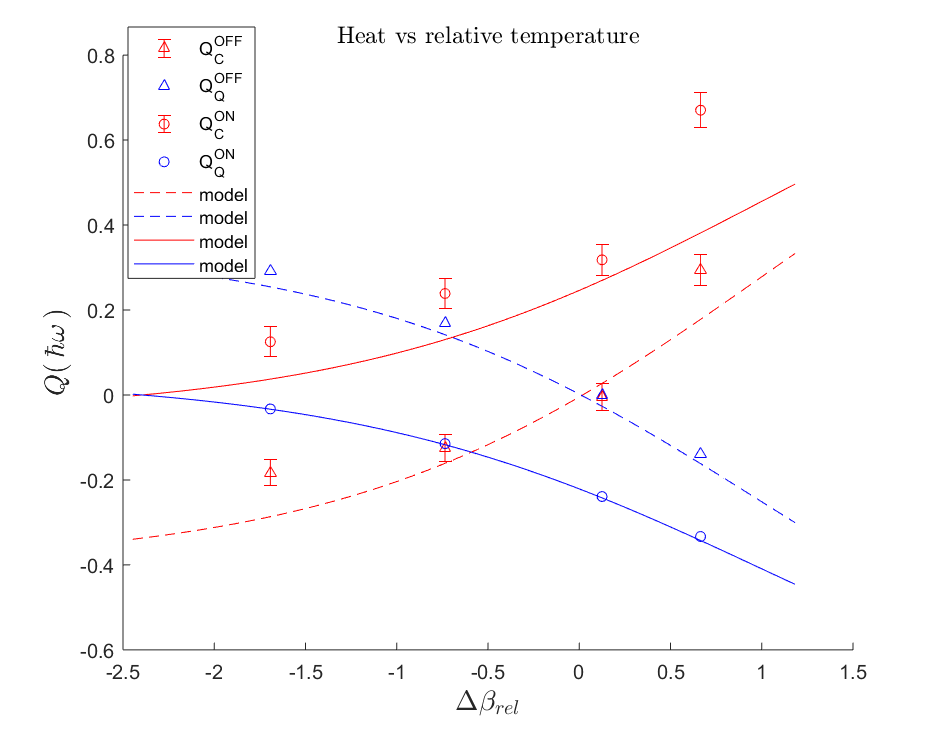
\includegraphics[height=0.45\textheight]{plots/Heat1.png}
  \caption{Plot of the exchanged heat depending on the Maxwell demon state ($ON$
    or $OFF$)}\label{fig:heat1}
\end{figure}

\begin{figure}
  \centering
  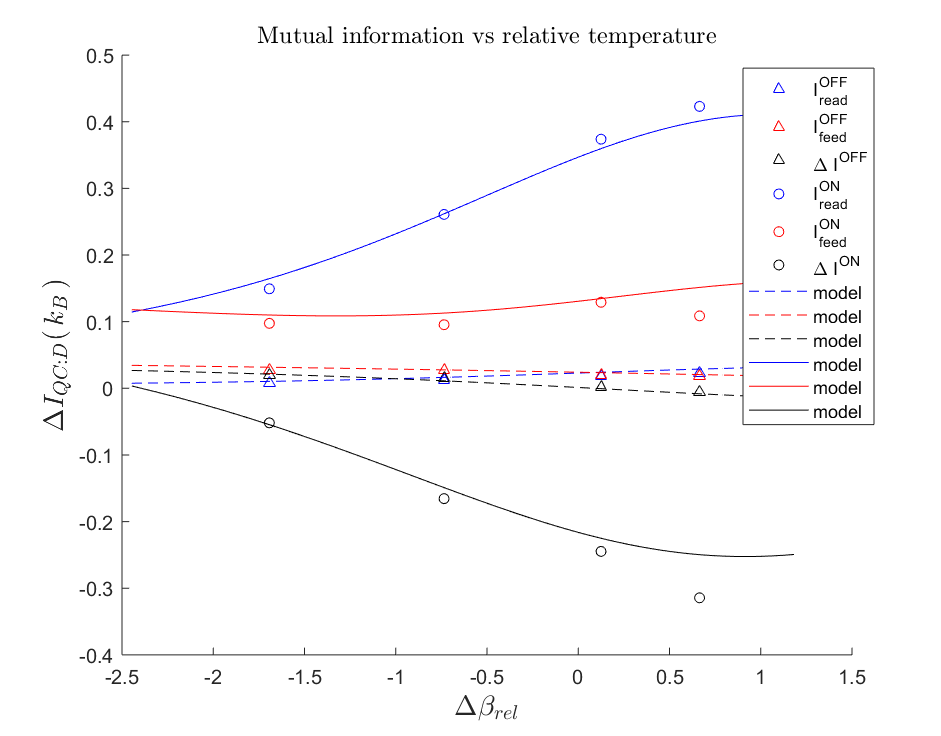
\includegraphics[height=0.45\textheight]{plots/Info1.png}
  \caption{Plot of the mutual information in the readout phase vs the feedback
    phase}\label{fig:info1}

\end{figure}

\begin{figure}
  \centering
  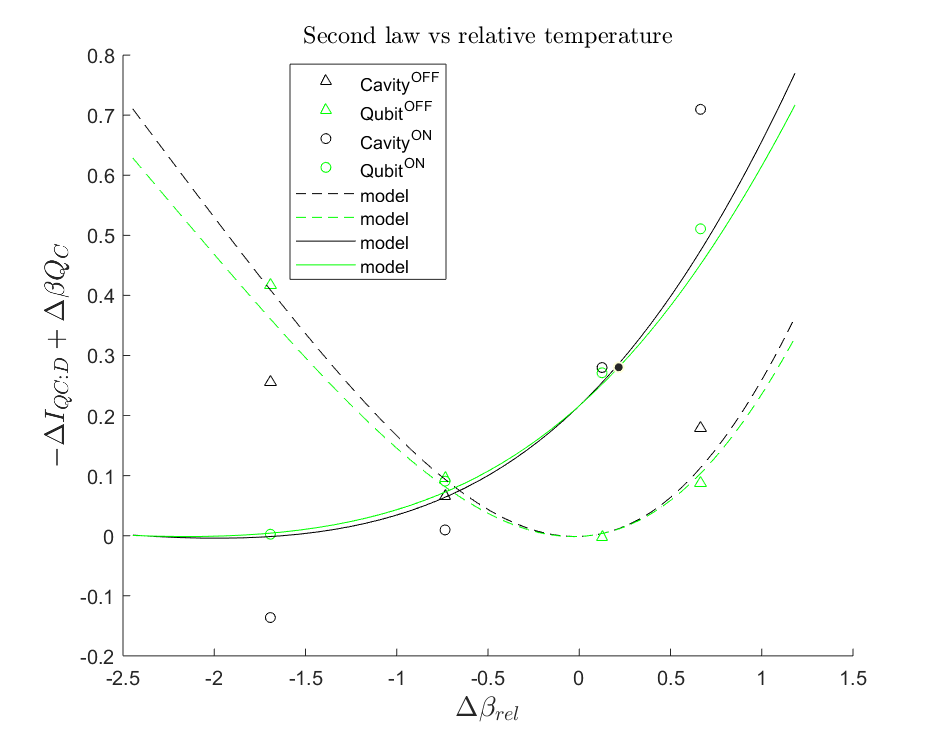
\includegraphics[height=0.45\textheight]{plots/Weak1.png}
  \caption{Plot of the weak second law in \cref{eqn:weaksnd}}\label{fig:weak1}
\end{figure}

\begin{figure}
  \centering
  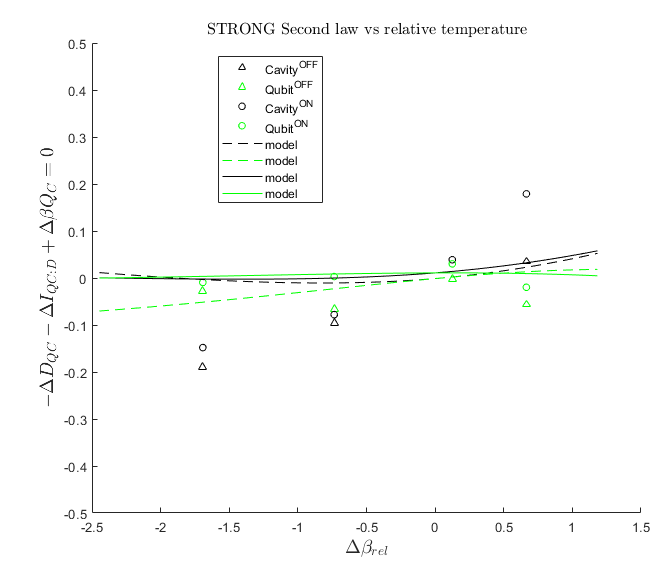
\includegraphics[height=0.45\textheight]{plots/Strg1.png}
  \caption{Plot of the strong second law in \cref{eqn:strgsnd}}\label{fig:strg1}
\end{figure}

\chapter{Error estimation and validity proofs}

As seen in the previous chapter most of our thermodynamics quantities involve
directly or indirectly entropy or other statistical quantity of the density
matrix. However the proof of validity in~\cite{SPRAL17} only covers the case of
observable i.e function such as $f(\rho) = \Tr(\rho A)$ with $A \in
\mathcal{O}(\mathcal{H})$. In our case the entropy is not observable, it is not even
linear. It depends not on quantum properties but on the statistical part of the
density matrix. And even worse, its derivative goes to infinity on the edge of
$\mathcal{D}$.

The two problems I have to solve are then:
for a generic function $f : \mathcal{D}
\to \R$,
\begin{itemize}
\item Is the average value of $f(\rho)$ indeed $f(\rho\ml)$?
\item How to compute the error of value of such general $f$ on the reconstructed
  matrix as \cref{eqn:var} does not work?
\end{itemize}

My first approach to solve the second problem was a Monte-Carlo simulation
explained in \cref{sec:MC}. It gave quite good results especially since,
before this, the team had absolutely no idea of the error of various
entropy-related values. It was thus impossible to evaluate how a point a
bit off the theoretical curve fitted there.

However this first approach was filled with more or less wrong independence
hypothesis (I was forced to assume independence nearly everywhere). So I dived
into~\cite{SPRAL17} and proved the first point to be true and found a way to
adapt \cref{eqn:var} to our case.

In the end another problem was that, as explained in \cref{ssec:uniq}, if
$\Span(E_i)$ is not the full space, the solution is not unique. We need a way to
pick the ``best solution''. As this is not well defined I propose two possible
definitions, both based on maximizing a score function, in \cref{sec:fixspan}.

\section{Quick approach: Monte-Carlo estimation}\label{sec:MC}

At the beginning of my internship, I designed a Monte-Carlo algorithm to sample
the probability space according to the distribution deduced from the deviation on
each coefficient. The goal was to have a quick and dirty method to quickly get
error-bars that would have been a little but not too much wrongly estimated.

In order to do that, I had to create a probability distribution that matched the
deviation on each coefficient. But this distribution
cannot be sampled easily because it is the projection of density low on a
subvector-space. Let's look at the problem more formally.

In practice, in Luis' setup, we have only information on the
population from the reconstruction and we force the coherences to be 0.
The problem is just about probability vectors on the diagonal.
So our input is a set of values
$p_i$ and deviations $\Delta p_i$ such that each $p_i$ marginal law is a normal
law. In theory the probability distribution on $\R^n$ is:

\[\dd p(x_1,\ldots,x_n) = K \exp\left(\sum \frac{(x_i - p_i)^2}{2\Delta p_i^2}
  \right) \dd(x_1,\ldots,x_n)\]

where $K$ is a normalization constant. However, the vector $x =(x_1,\ldots,x_n)$
must be positive and of sum 1. We'll call $\mathcal{P}_n$ the set of probability
vectors of dimension $n$. We will define our new law on $\mathcal{P}_n$ by the
same density function but on top of the Lebesgue measure of dimension $n-1$.
This distribution is much harder to simulate because it is both projected and
truncated ($\mathcal{P}_n$ is not the whole hyperplane of sum $n$).

In order to do the sampling, I use an adapted hit and run method to build a
Markov chain on $\mathcal{P}_n$ whose stationary
distribution is the wanted distribution. The idea is very simple: I know how to
truncate a Gaussian law to a segment and sample it on that segment. So an
iteration of the Markov chain is to go from the previous point $x_{n-1}$ and
sample a random direction in the hyperplane of sum 1. This direction and
$x_{n-1}$ give us an affine line of that hyperplane.

We can then compute the
intersection of that line and $\mathcal{P}_n$. Then we can project the
multivariate Gaussian law on the line. As we are working with normal laws, the
projected law will be normal and we just have to figure out the center and the
standard deviation. If we scale the whole space on each axis by the
corresponding $\Delta p_i$, this is just an orthogonal projection.

Once we have the law on the line and the segment, we sample the truncated law on
the segment and this gives us $x_n$. The wanted distribution is indeed a
stationary distribution of this Markov chain, and the chain fully mixes the set
$\mathcal{P}_n$. On discrete probability sets, this is sufficient to say that there
is only one stationary distribution and that the chain converges towards it. I
hope that this is still true for continuous chains. I decided that this is an inexact
and informal way to get the deviation on our function and so spending more time
on it to have strong convergence results
instead of doing the work of the next section was not a good idea.

If I assume that the chain indeed converges toward the right probability
distribution, then by sampling this chain long enough, I
can get the statistic average and standard deviation of any real function of
$\mathcal{P}_n$. This give good enough error bars for our purposes.

\section{Complete first order error-bars}\label{sec:errbar}

In this section I try to formalize and prove formulas for getting the
expectation and standard deviation of any function on the set of density
matrices $\mathcal{D}$ following the probability given by the maximum-likelihood
reconstruction.

All the theorems in this section are generalizations,
adaptations, and improvements from~\cite{SPRAL17}. The goal here is to compute
the expected value and the variance of a generic function $h : \mathcal{D} \to
\R$ on a variable $\rho$ following a prior distribution $P_0$
knowing all the measurement
we did. If $\Span E_i$ is the full space,
we will prove that when the number $N$ of measurement go to infinity, the
expectation is
\[E(h(\rho)) = h(\rho\ml) + O(N\inv)\]

and the variance is:
\[V(h(\rho)) = \Tr(\nabla h\pr \mathbb H\inv(\nabla h\pr)) +O(\frac 1 {N^2})\]

Where $\nabla h$ is the gradient of $h$ on the set of Hermitian
matrices of null-trace, and $A\pr$ and $\mathbb H$ are the same as below
\cref{eqn:var}. Both asymptotic value are independent of $P_0$. It is important
to note that the term $O(\frac 1 N^2)$ in the variance formula
is still an order of magnitude below
the main term because the variance will decrease in $\frac 1 N$ when the number
of experiments increase.

One can check that if we set
$h(\rho) = \Tr(A\rho)$, we'll find back the result of \cref{sec:basicerr}.

Obviously some
regularity condition that will be given later are needed on $h$ for those result
to work.
I tried and achieved to have quite low regularity conditions so that people could
use those result with low-regularity functions. However those conditions are not
sufficient to deal with the entropy on the edge of $\mathcal{D}$. In
\cref{sec:regentropy}, I explain how one can achieve similar results with the
entropy, but with other terms less bound: $E(h(\rho)) = h(\rho\ml) +
O(N^{-\varepsilon})$ for $\varepsilon < 1$.

\

Let's formalize how to prove those asymptotic. For simplicity we'll assume that
$P_0$ can be expressed as a density function on the Lebesgue measure of the
$\Tr = 1$ hyperplane. With that out of the way, we can study the modification of
$P_0$ thanks to the measurements we did by the means of the likelihood function.
$\mathcal{L}(\rho) = e^{\ell(\rho)}$ is the density of probability of having
the measurements we had, given the density matrix $\rho$. Therefore, according to
Bayes law (see \cref{eqn:bayes}), we have
\[E(h(\rho)) = \frac{I_h}{I_1}\]
where:
\[I_h = \int h(\rho) e^{\ell(\rho)} P_0(\rho) \dd \rho \]

However to do asymptotic we need to grow a single variable. Thus, we'll write our
asymptotic development as if we repeat the experiment and get again the same
results. The log-likelihood function will then be $N\ell$. We'll assume that this
give the same asymptotic behavior as if we grew the number of measurements inside
$\ell$. The number of repetition that'll grow to infinity will thus be $N$, so we
will write:
\[E_h(N) = \frac{I_h(N)}{I_1(N)}\]
where:
\[I_h(N) = \int h(\rho) e^{N\ell(\rho)} P_0(\rho) \dd \rho \]

ans study $E_h(N)$ as $N \to \infty$. To compute variances, we only need to get
the expectation of:
\[h_V = \left(h - \lim_{N \to \infty} E_h(N)\right)^2\]



\subsection{Full rank}

We'll start by studying what happens when $\rk \rho\ml = n$ i.e when $\rho\ml$
is in the interior of $\mathcal{D}$. In order to that, we new a few technical theorems.

\begin{thm}\label{thm:asy1}
  Let $g : U \to \R$ be a function of class $\class 1$ on $U$ a neighborhood of 0. If $g(0)
  \neq 0$, we have at $N \to \infty$:
  \[\int_{z \in U} g(z)e^{-\frac N2\|z\|^2} \dd z = g(0){\left(\frac
      {2\pi}{N}\right)}^{\frac n 2} +
    O\left({N^{-\frac n 2 -1}}\right)\]
\end{thm}

\begin{proof}

  We can decompose $g$ in $g(z) = g(0) + h(z)$ with $h(z) = O(\|z\|)$ as $g$ is
  $\class{1}$ in 0, thus:
\[\int_{z \in U} g(z)e^{-\frac N2\|z\|^2} \dd z = g(0)\int_{z \in U} e^{-\frac
    N2\|z\|^2} \dd z + \int_{z \in U} h(z)e^{-\frac N2\|z\|^2} \dd z\]

But:
\begin{align*}
  \left |\int_{z \in U} h(z)e^{-\frac N2\|z\|^2} \dd z\right|
  &\leq C \int_{z \in U} \|z\|e^{-\frac N2\|z\|^2} \dd z\\
  &\leq C \int_{z \in \R^n} \|z\|e^{-\frac N2\|z\|^2} \dd z\\
  &\leq CA_n \int_{r \in \R_+} r^{n+1}e^{-\frac N2 r^2} \dd r\\
  &\leq CA_n \int_{r \in \R_+} r^{n+1}e^{-\frac N2 r^2} \dd r\\
  &\leq O\left({N^{-\frac n 2 -1}}\right)
\end{align*}

Where $C$ is the constant such that $|h(z)| \leq C \|z\|$, $A_n$ is the surface
of the hypersphere of $\R^n$ and the last line comes from \cref{eqn:gausspown}.

Up to exponentially small terms ($O(e^{N\delta})$ for a given $\delta$), we have
(using \cref{eqn:gaussdimn}):

\[g(0)\int_{z \in U} e^{-\frac
    N2\|z\|^2} \dd z \approx g(0)\int_{z \in \R^n} e^{-\frac
    N2\|z\|^2} \dd z = g(0) {\left(\frac
      {2\pi}{N}\right)}^{\frac n 2}\]

\end{proof}

\


However when $g(0) = 0$, the previous theorem does not give anymore the first
order term but just a bound on the integral which may not be very useful in
certain cases. We'll thus look in more details at the case $g(0) = 0$. We'll
assume additionally that $\nabla g = 0$, because that is what happens for our
cases that require that theorem.


\begin{thm}\label{thm:asy2}
 Let $g : U \to \R$ be a function of class $\class 3$ on $U$ a neighborhood of 0. If $g(0) = 0$
 and $\nabla g(0) = 0$, We have at $N \to \infty$:
  \[\int_{z \in U} g(z)e^{-\frac N2\|z\|^2} \dd z = \frac{\Tr(\nabla^2 g(0))}{2N} {\left(\frac
        {2\pi}{N}\right)}^{\frac n 2} +
    O\left({N^{-\frac n 2 -2}}\right)\]
\end{thm}

\begin{proof}
  $g$ can be written $g(z) = \frac12\bra z \nabla^2 g(0) \ket z + O(\|z\|^3)$ because it
  is $\class 3$. The integral on the $O(\|z\|^3)$ part gives $O\left({N^{-\frac
        n 2 -2}}\right)$ with \cref{eqn:gausspown} with the same method as in
  the precedent proof.

  We can then use \cref{lem:gausssymtr} to get the result.
\end{proof}

\

Up until now, we used a simple Gaussian in the exponential, but in practice,
what we want in there is our log-likelihood function $\ell$, let's do a generic
theorem then:

\begin{thm}\label{thm:asymid}
  Let $U$ be an open set containing $0$. Let $f : U \to \R$ be a $\class 4$ function.
  Let $g : U \to \R$ be a $\class 1$ function.
  Assume that $f$ has a unique global non critical maximum in $0$
  ($\nabla f = 0$ and $\nabla^2 f < 0$). We have at $N \to \infty$:
  \[\int_{z \in U} g(z)e^{Nf(z)} \dd z = g(0)
    {\left(\frac {2\pi}{N}\right)}^{\frac n 2}
    \frac {e^{Nf(0)}}{\sqrt{\left|\det \nabla^2 f(0)\right|}}
    + O(e^{Nf(0)} N^{-\frac n 2 -1})\]

  Additionally, If $g(0) = 0$ and $\nabla g(0) = 0$, and $f \in \class 6$ and $g
  \in \class 3$, we have:

  \[\int_{z \in U} g(z)e^{N f(z)} \dd z =
    \frac{\Tr\left(-\nabla^2 g(0) {\left(\nabla^2 f(0)\right)}^{-1}\right)}{2N}
    {\left(\frac {2\pi}{N}\right)}^{\frac n 2}
    \frac {e^{Nf(0)}}{\sqrt{\left|\det \nabla^2 f(0)\right|}}
    + O\left(e^{Nf(0)}{N^{-\frac n 2 -2}}\right)\]
\end{thm}

\begin{proof}
First we assume $f(0) = 0$ without loss of generality (it suffice to divide
everything by $e^{Nf(0)}$). The Morse lemma (\ref{lem:morse}) tells us that
there is a $V \in \mathcal{N}(0)$ and
a diffeomorphism $\psi : V \to V'$ with $\psi(0) = 0$ such that
\[f(z) = - \frac12 \|\psi(z)\|^2 \gap \text{and}\gap \nabla \psi(0) =
  \sqrt{-\nabla^2 f}\]

Because the hessian of $f$ is negative definite in 0 and the maximum is unique,
all values of $f$ outside of $V$ are below a
constant $-\delta$. So all the part of the integral outside of $V$ are
$O(e^{-N\delta})$ and thus negligible. We can now study the integral only on
$V$. We can then make a change of variable on $\psi$:

\[\int_{z \in V} g(z)e^{Nf(z)} = \int_{z \in V'}
  g(\psi^{-1}(z))e^{-\frac N2\|z\|^2} J(z) \dd z\]

with $J(z) = |\det{\nabla \psi^{-1}}|$. We can then set $g_0(z) =
g(\psi^{-1}(z))J(z)$, and look at the two cases:
\begin{itemize}
  \item As $f \in \class 4$, we have $\psi \in \class 2$ (and thus also
    $\psi^{-1}$) and finally $J \in \class 1$, but $g$ is also in $\class 1$, so
    $g_0$ is in $\class 1$. We can then apply \cref{thm:asy1} and get the result
    we want with:
\[g_0(0) = g(\psi^{-1}(0))J(0) = g(0)\frac 1 {\det {\nabla \psi(0)}} =
  \frac {g(0)}{\sqrt{\left|\det \nabla^2 f\right|}}
  \]


  \item As $f \in \class 6$, we have $\psi \in \class 4$ (and thus also
    $\psi^{-1}$) and finally $J \in \class 3$, but $g$ is also in $\class 3$, so
    $g_0$ is in $\class 3$. We can then apply \cref{thm:asy2} and get the result
    we want with:
    \[\nabla g_0^t = \nabla g^t \nabla \psi\inv \times J + g \circ \psi\inv
      \times \nabla J\]
    but as $g(0) = 0$, we have $g(\psi^{-1}(0)) = 0$ and furthermore $\nabla
    g(0) = 0$ so $\nabla (g \circ \psi^{-1})(0) = 0$. Finally, the only remaining term is:
    \begin{align*}
      \nabla^2 g_0(0))
      &= \nabla^2 (g \circ \psi\inv) \times J(0)\\
      &= {(\nabla \psi^{-1}(0))}^t\nabla^2 g(0) {(\nabla \psi^{-1}(0))} \times
         \frac {1}{\sqrt{\left|\det \nabla^2 f\right|}}
    \end{align*}
    If we put that to the trace, we get the result we wanted.

\end{itemize}

\end{proof}

\subsection{Partial rank}

When $\rho\ml$ is not of full rank, we are on the edge of $\mathcal{D}$. We must
thus study what happens to the results of the previous section, when we are on
the edge. Luckily, we can just study the case of edges on which only one
dimension is missing. Indeed when more dimension are missing, there is a trick
to bring it back to only one dimension missing.

\begin{rem}
All formulas here work
with only $x$ i.e if $n$, the dimension of $z$, is 0. It suffice to note that the
Lebesgue measure of the point is 1 and all the proofs work.
\end{rem}

\begin{thm}\label{thm:asyp1}
  Let U be an open set of $\R_+ \times \R^n$ where $(0,0) \in U$. The $\R_+$
  coordinate will be $x$ and the $\R^n$ coordinate will be $z$. Let $g : U \to
  \R$ by a $\class 1$ function. The derivative against the edge i.e on $x$ are
  taken as one-sided derivative. We have as $N \to \infty$:

  \[\int_{(x,z) \in U} x^m g(x,z)e^{-N(x + \frac 12 \|z\|^2)} \,\dd x\, \dd z =
    g(0,0)\,m! {(2\pi)}^{\frac n 2} N^{-\frac n 2 - m - 1} + O(N^{-\frac n 2 - m - 2})\]
\end{thm}

\begin{proof} With the now usual argument, we can restrict ourselves to a
  rectangular set $U' = [0,\eta) \times U_z \subset U$.
  Here we decompose $g$ in $g(x,z) = h(z) + x g_1(x,z)$ with $h(z) = g(0,z)$ (We
  can do that because $g$ is $\class 1$). As
  $g_1$ is bounded on $U$, we have:
\begin{align*}
  \int_{(x,z) \in U'} x^{m+1}g_1(x,z)e^{-N(x + \frac 12 \|z\|^2)} \,\dd x\, \dd z
  &\leq
  \|g_1\|_\infty\int_{(x,z) \in U'} x^{m+1}e^{-N(x + \frac 12 \|z\|^2)} \,\dd x\, \dd z\\
    &=O(N^{-\frac n 2 - m - 2})
\end{align*}

This is because we can split the integral and use \cref{eqn:gaussdimn} and \cref{eqn:gamma}\\
On the other hand, thanks to \cref{eqn:gaussdimn} and \cref{thm:asy1}, we have:
\begin{align*}
  \int_{(x,z) \in U'} x^{m}h(z)e^{-N(x + \frac 12 \|z\|^2)} \,\dd x\, \dd z
  &= \int_0^\eta x^{m}e^{-Nx} \,\dd x \times
    \int_{z \in U_z} h(z)e^{-\frac N2 \|z\|^2} \, \dd z\\
  &= m! N^{-m-1} \times( h(0){\left(\frac
      {2\pi}{N}\right)}^{\frac n 2} +
    O\left({N^{-\frac n 2 -1}}\right))
\end{align*}

\end{proof}


\begin{thm}\label{thm:asyp2}
  If we add to the previous theorem the hypothesis that $g(0) = 0$, $\nabla g(0) =
  0$ and $g$ is $\class 2$ and in particular $\class 3$ on the
  variable $z$ (i.e.\ for any $x$, $z \mapsto g(x,z) \in \class 3$), we have:
  \[\int_{(x,z) \in U} x^m g(x,z)e^{-N(x + \frac 12 \|z\|^2)} \,\dd x\, \dd z
    = \frac{m!\Tr\left(\dparn g z 2\right)}{2N^{m+2}}
    {\left(\frac {2\pi}{N}\right)}^{\frac n 2}
    + O\left({N^{-\frac n 2 -m -3}}\right)\]
\end{thm}

\begin{proof}
  We use the same $U'$ as in last proof.
  By applying \cref{lem:dec} twice, we get
  \[g(x,z) = h(z) + x^2g_2(x,z)\]
  For that same reason as in previous proof, The integral on $x^2g_2$ is
  $O(N^{-\frac n2 - m - 3})$. We can then, like the previous proof, split the
  integral and use \cref{eqn:gaussdimn} and \cref{thm:asy2} to get the result.
\end{proof}

Like in the previous section we now need to take care about a generic function
$f$ in the exponential. We can't use the \cref{thm:asymid} because it assume a
null gradient for $f$ but here $\dpar f x$ could be negative.

\begin{thm}\label{thm:asypmid}
   Let U be an open set of $\R_+ \times \R^n$ where $(0,0) \in U$. The $\R_+$
  coordinate will be $x$ and the $\R^n$ coordinate will be $z$. Let $f:U \to \R$
  be a function of class $\class 4$ and $g : U \to
  \R$ be a function of class $\class 1$. The derivative against the edge i.e on $x$ are
  taken as one-sided derivative. Assume that $f$ has a global non-critical
  maximum in $0$ so that $\dpar f z(0) = 0$ and $\dparn f z 2(0) < 0$. Furthermore, we
  assume that $\dpar f x(0) < 0$. We have as $N \to \infty$:
  \[\int_{(x,z) \in U} x^m g(x,z)e^{Nf(x)} \,\dd x\, \dd z =
    \frac{g(0,0)\,m! {(2\pi)}^{\frac n 2}}{N^{\frac n 2 + m + 1}} \times
    \frac{e^{Nf(0,0)}}
    {\sqrt{\left|\det \dparn f z 2\right|} \left(-\dpar f x\right)^{m+1}}
    + O(e^{Nf(0,0)}N^{-\frac n 2 - m - 2})\]

  Additionally, if $g(0) = 0$, $\nabla g(0) = 0$, $g$ is $\class 2$ and in
  particular $g$ is $\class 3$ on
  variable $z$ and $f$ is $\class 6$, We have as $N \to \infty$:
   \[\int_{(x,z) \in U} x^m g(x,z)e^{Nf(x)} \,\dd x\, \dd z
    = \frac{m!\Tr\left(\dparn g z 2 \left( \dparn f z 2 \right)\inv\right)}{2N^{m+2}}
     \times
    \frac{{\left(\frac {2\pi}{N}\right)}^{\frac n 2}e^{Nf(0,0)}}
    {\sqrt{\left|\det \dparn f z 2\right|} \left(-\dpar f x\right)^{m+1}}
    + O\left(e^{Nf(0,0)}{N^{-\frac n 2 -m -3}}\right)\]
\end{thm}

\begin{proof}
  We start by supposing $f(0,0) = 0$ by dividing everything by $e^{Nf(0,0)}$.

  We now do a change a variable to bring back $f$ to be $-x -\frac12\|z\|^2$ like in
  the proof of \cref{thm:asymid}.
  To that change of variable we decompose $f$ in $f(x,z) = h(z) + xf_1(x,z)$
  with $h(z) = f(0,z)$. The change of variable $\tilde x = xf_1(x,z)$ and
  $\tilde z = \psi(z)$ where $\psi$ is the Morse lemma decomposition of $h$ will
  give the right result. Doing the actual variable change and computing the
  Jacobian is left to the reader.
  The regularity analysis is the same as in \cref{thm:asymid}
\end{proof}



\subsection{Application}

Here we can finally apply all those asymptotic theorem to our case. I first recall the
notations. For $h : \mathcal{D} \to \R$, we note:
\begin{equation}
I_h(N) = \int_{\rho\in\mathcal{D}} h(\rho) e^{N\ell(\rho)} P_0(\rho) \dd \rho
\end{equation}
Where $P_0$ is the prior probability distribution on density matrices.
So that we have its expectation:
\begin{equation}
E_h(N) = \frac{I_h(N)}{I_1(N)}
\end{equation}
Its variance is the expectation of:
\begin{equation}
h_V = {\left(h - \lim_{N \to \infty} E_h(N)\right)}^2
\end{equation}

We make some technical assumptions such as:
\begin{itemize}
\item $P_0(\rho\ml) > 0$: If our estimator has a null-probability, the prior
  distribution doesn't make much sense.
\item $P_0$ is of class $\class 3$: This is necessary for the various asymptotic developments.
\item $\mathcal{D} = \mathcal{D}(\C^d)$: We use simple $d$-dimensional density matrices.
\end{itemize}


\begin{lem}\label{lem:asymain}
  For any $h$ of class $\class 1$ on $\mathcal{D}$, we have:
  \[E_h(N) = h(\rho\ml) + O\left(\frac 1N\right)\]
  and for any $h$  of class $\class 2$ such that $h(\rho\ml) = 0$, $\nabla
  h(\rho\ml) = 0$, and such that,
  if we name $z$ the variable on the space tangent to $\mathcal{D}_{\rk
    \rho\ml}$ in $\rho\ml$, $g$ is of class $\class 3$ in $z$, we have:
  \[E_h(N) = \frac{\displaystyle \Tr \left( - \dparn h z 2 (\rho\ml)  \left( \dparn \ell z
        2(\rho\ml)\right)\inv\right)}{2N} + O\left(\frac 1 {N^2}\right)\]
\end{lem}

\begin{proof}[Proof if $\rho\ml$ has full rank]
  In this case, $D$ is a neighborhood of $\rho\ml$ in the hyperplane of
  Hermitian matrices of trace 1.
  This hyperplane is itself an euclidean real vector space isometric to $\R^n$
  for a given $n$. $\ell$ is
  smooth so it is $\class 4$, and it has a global unique (by convexity)
  non-critical (by strong convexity) maximum in $\rho\ml$. As both $h$ and $P_0$
  are of class $\class1$, we can just do a translation to apply
  \cref{thm:asymid}. We have then:
  \[I_h(N) = h(\rho\ml)P_0(\rho\ml)
    {\left(\frac {2\pi}{N}\right)}^{\frac n 2}
    \frac {e^{N\ell(\rho\ml)}}{\sqrt{\left|\det \nabla^2 f(\rho\ml)\right|}}
    + O(e^{N\ell(\rho\ml)} N^{-\frac n 2 -1})\]
  and
  \[I_1(N) = P_0(\rho\ml)
    {\left(\frac {2\pi}{N}\right)}^{\frac n 2}
    \frac {e^{N\ell(\rho\ml)}}{\sqrt{\left|\det \nabla^2 f(\rho\ml)\right|}}
    + O(e^{N\ell(\rho\ml)} N^{-\frac n 2 -1})\]
  Everything then simplifies in the result we wanted:
  \[E_h(N) = \frac{I_h(N)}{I_1(N)} = h(\rho\ml) + O\left(\frac 1N\right)\]

  In second case $h(\rho\ml) = 0$, $z$ just span the full space and so represent
  the same variable as $\rho$. Therefore $h$ is just plainly $\class 3$, we can
  thus just apply the second part of \cref{thm:asymid}, and get:
  \[I_h(N) =
    \frac{\Tr\left(-\nabla^2 h(\rho\ml) {\left(\nabla^2 \ell(\rho\ml)\right)}^{-1}\right)}{2N}
    {\left(\frac {2\pi}{N}\right)}^{\frac n 2}
    \frac {e^{N\ell(\rho\ml)}}{\sqrt{\left|\det \nabla^2 f(\rho\ml)\right|}}
    + O\left(e^{Nf(0)}{N^{-\frac n 2 -2}}\right)\]
  And finally:

  \[E_h(N) = \frac{I_h(N)}{I_1(N)} =
    \frac{\Tr\left(-\nabla^2 h(\rho\ml) {\left(\nabla^2
            \ell(\rho\ml)\right)}^{-1}\right)}{2N}
    + O\left(\frac 1{N^2}\right)\]







  % This proof comes straight from~\cite{SPRAL17}. The only thing added would be
  % to check all the regularity conditions which I have only done informally on paper yet.
  % I'll try to do that by Monday night.
\end{proof}

\begin{proof}[Proof if $\rho\ml$ has partial rank and $\nabla \ell \neq \lambda I$]
  This proof is a bit more subtle, because in \cref{thm:asypmid}, the edge
  dimension $x$ is of only one dimension but here, we may miss several
  dimensions. We thus need to mount a change of variable that reduces several
  dimension to one. This change of variable came form~\cite{SPRAL17}.

  Before starting let's just name $h_0(\rho) = h(\rho)P_0(\rho)$.

  First let $r$ be the rank of $\rho\ml$. Then let's suppose that $\rho\ml$ is
  diagonal by rotating everything along a unitary $U$ such that $\rho\ml = U
  DU^\dagger$. $D$ will then be $\mathrm{diag}(0,\ldots,0,p_1,\ldots,p_r)$.
  We'll define $\Delta$ by:
  \[ D = \mat{0 & 0\\0&\Delta}\]

  We can then
  pose the following change of variable:
  \begin{equation}
  \Psi(\xi,\zeta,\omega) = \exp\mat{0 &\omega\\-\omega^\dagger&0}
    \mat{\xi&0\\0&\Delta + \zeta - \Tr \xi \frac{I}r} \exp\mat{0 &-\omega\\\omega^\dagger&0}
  \end{equation}

  Where $\xi \in \mathcal{O}(\C^{d-r})$, $\omega \in \mathcal{M}_{(d-r),r}$ and
  $\zeta \in \mathcal{O}(\C^r)$ but with $\Tr \zeta = 0$. First, let's show that
  it is a diffeomorphism. We have:
  \begin{equation}
    \nabla \Psi(D) \cdot (\delta\xi,\delta\zeta, \delta\omega) =
    \mat{\delta\xi& \delta\omega\,\Delta\\ \Delta\, \delta\omega & \delta\zeta -
      \Tr(\delta\xi)\frac Ir}
  \end{equation}
  This is bijective ($\Delta$ is invertible), so by local inversion theorem
  $\Psi : U \to V$ is a diffeomorphism on $V$ a neighborhood of $D$. By the
  same argument as usual, we can focus our study of the various integral to only
  $U' = U \cap \mathcal{D}$ and even to $U'' = \mathring U'$ because $U'
  \setminus U''$ is of null measure. We can thus apply the change of variable
  \newcommand{\vars}{(\xi,\zeta,\omega)}
  \newcommand{\dvars}{\dd \xi\, \dd \zeta\, \dd \omega\,}
  \newcommand{\pvars}{\Psi(\xi,\zeta,\omega)}
  \begin{equation}\label{eqn:uglyint}
    \int_{\rho \in U''} h_0(\rho)e^{N\ell(\rho)}\dd \rho =
    \int_{\vars \in V''} h_0(\pvars)e^{N\ell(\pvars)}J\vars \dvars
  \end{equation}
  Where $J(\vars)$ is the determinant of the Jacobian of $\Psi$ and $V'' = \Psi(U'')$.

  In fact we can characterize what the edge of $\mathcal{D}$ is in the
  $\vars$-space:
  \[\rho = \pvars > 0 \iff \xi >0\]

  So we would like $\xi$ to be our $x$ variable and $(\zeta,\omega)$ to be our
  $z$ variable. On one hand the second part is easy: let's name $z$ the variable
  $z = (\zeta,\omega)$. One the other hand the first part is not that easy
  because $\xi$ is multidimensional (except if $r = n-1$).

  Luckily If we write $\xi = x \sigma$ with $\sigma \in \mathcal{D}(\C^{d-r})$,
  we'll have $\xi > 0 \iff x > 0$ and we are brought back to a single one sided
  variable. If we name $\Phi(x,\sigma) = x \sigma$ our function, it is a
  diffeomorphism on the whole $\R_{>0} \times \mathcal{D}(\C^{d-r})$ to the positive
  definite Hermitian matrices of size $r$. Furthermore it's Jacobian can easily
  be computed and it is $x^r$.

  There just one problem before doing a new change
  of variable: In order to do a proper change of variable, we'll
  need to split $\xi$ from $z$, Thus we'll build a rectangle
  neighborhood $V'''$ of
  $(0,0,0)$ that separates $\xi$ on one side and $z$ on the other,
  such that $V''' = V'''_\xi \times V'''_z$.
  We'll also use $W''' = \Phi\inv(V'''_\xi)$ We'll thus have:
  \newcommand{\ppvars}{\Psi(\Phi(x,\sigma),z)}
  \newcommand{\pvvars}{(\Phi(x,\sigma),z)}
  \newcommand{\pdvars}{\dd x\, \dd \sigma\, \dd z}
  \begin{multline}
    \int_{\rho \in U'''} h_0(\rho)e^{N\ell(\rho)}\dd \rho =\\
    \int_{(x,\sigma) \in W'''}\int_{z \in V'''_z} x^m h_0(\ppvars)e^{N\ell(\ppvars)}J\pvvars
    \,\pdvars
  \end{multline}

  Where $m = \dim \mathcal{D}(\C^{d-r}) = (d-r)^2 -1$.
  If we split again $W'''$ in a rectangular sub-neighborhood of $0$, namely $W''''_x \times
  W''''_\sigma$, we have:

  \begin{multline}
    \int_{\rho \in U''''} x^m h_0(\rho)e^{N\ell(\rho)}\dd \rho =\\
    \int_{\sigma \in W''''_\sigma}\left(  \int_{(x,z) \in W''''_x \times V'''_z}
      h_0(\ppvars)e^{N\ell(\ppvars)}J\pvvars \,\dd x \, \dd z
    \right) \dd \sigma
  \end{multline}

  We now want to apply \cref{thm:asypmid} on the integral inside the
  parenthesis. Let's check all the hypothesis. $U = \overline{W''''_x \times
    V'''_z}$ is a neighborhood of $(0,0)$ in $\R_+ \times \R^n$.
  $\ell, \Psi, \Phi$ are smooth so
  $f(x,z) = \ell(\ppvars)$ will be $\class 4$. Be a non-critical global maximum
  is conserved when pare-composing with any differentiable function so $(0,0)$ is global maximum
  of $f$ on $U$.

  We now only need to prove about $f$ that $\dpar f x < 0$:
  \[\dpar f x \times \delta x = \nabla \ell \cdot \mat{\delta x\, \sigma & 0\\0 &-
      \delta x I} \]

  According to \cref{prop:caracKKT} If $\nabla f \neq \lambda I$, we have $\eta
  \neq 0$ with $\eta \geq 0$ such that $\Tr(\eta D) = 0$ and $\nabla f + \eta =
  \lambda I$, Thus we have:
  \begin{equation}\label{eqn:etanu}
  \eta = \mat{\nu&0\\0&0}
  \end{equation}

  with $\nu \geq 0$ and $\nu \neq 0$. Therefore:
  \[\dpar f x = - \Tr(\eta\sigma) <0\]
  Additionally, $h$ and $P_0$ are $\class 1$, and $J$ is smooth so $g(x,z) =
  h_0(\ppvars)J\pvvars$ is of class $\class 1$. We can then
  apply~\cref{thm:asypmid}, and when $h(\rho\ml) \neq 0$ we have:

  \begin{equation}\label{eqn:IhNp}
    I_h(N) =
    \frac{h(\rho\ml)P_0(\rho\ml)J(0,0)\,m! {(2\pi)}^{\frac n 2}}{N^{\frac n 2 + m + 1}} \times
    \int_{\sigma \in W_\sigma''''}\frac{e^{N\ell(\rho\ml)}}
    {\sqrt{\left|\det \dparn f z 2\right|} \left(-\dpar f x\right)^{m+1}} \dd \sigma
    + O\left(\frac{e^{Nf(0,0)}}{N^{\frac n 2 + m + 2}}\right)
  \end{equation}

  We can then simplify everything and get the result we want.

  \

  In the case $h(\rho\ml) = 0$. We can easily check that the various regularity conditions
  are directly mapped on the similar conditions on $g$. Because $\dpar h z = 0$
  by hypothesis, we have:
  \[\dparn g z 2(0,0) = J(0,0)P_0(\rho\ml) \dparn h z 2 (\rho\ml)\]

  Therefore when we apply \cref{thm:asypmid} and simplify by \cref{eqn:IhNp},
  we get the second result we wanted.
\end{proof}


\

\

The corner case where the $\rho\ml$ is on the edge of $\mathcal{D}$ but the
gradient toward the exterior is 0 is not done in this report like in the original
paper~\cite{SPRAL17}. The probability that such an event happens is really low
(if it is not 0) in particular if we take into account the numerical errors of
the implementation. However it can still probably be done by splitting again the
$x$ and $z$ variable but keeping $x$ as a quadratic variable in the function in
the exponential.




\begin{thm}\label{thm:asymain}
  For any $h : \mathcal{D} \to \R$ of class $\class 1$,
  we have its expectation:
  \[E_h(N) = h(\rho\ml) + O\left(\frac 1N\right)\]
  Additionally, if it is of class $\class 3$ in the inside and along the edges
  and $\class 2$ otherwise with $\dparn h x 2 =
  o(\frac 1 x)$ when leaving the edge (where $x$ is a scalar variable coming from the
  edge), we'll have the variance:
  \[V_h(N) = E_{h_V}(N) = \frac{\Tr(\nabla h\pr \mathbb H\inv(\nabla h\pr))}N +O(\frac 1 {N^2})\]
  where:
\begin{itemize}
\item $\mathcal{D}_r$ is the submanifold of $\mathcal{D}$ of matrices with rank $r$
\item $A\pr$ is
  the orthogonal projection on the tangent space to $\mathcal{D}_{\rk \rho}$ in
  $\rho$:
  \[A\pr = A - \frac{\Tr(AP\ml)}{\Tr(P\ml)}P\ml - (I-P\ml)A(I-P\ml)\]
\item $\mathbb H$ is the hessian of $\ell_{|\mathcal{D}_{\rk \rho}}$ in $\rho$:
  \[\mathbb{H}(A) = \sum_i \frac{\Tr(A{E_i}\pr)}{\Tr^2(\rho\ml E_i)} {E_i}\pr +
    (\lambda I - \nabla \ell(\rho\ml))A\rho\ml^+ +
    \rho\ml^+A(\lambda I - \nabla \ell(\rho\ml))\]
  Where $\rho^+$ is the Moore-Penrose pseudo inverse.
\end{itemize}

\end{thm}

\begin{proof}
  The expectation proof is just direct application of \cref{lem:asymain}. For
  the variance, it's a bit more tricky. First, let's check the regularity
  conditions. We want to apply \cref{lem:asymain} on $h_v = {\big(h - h(\rho\ml)\big)}^2$.
  On the inside $h$ is of class $\class 3$, so we have

  \begin{equation}\label{eqn:hvder}
  \nabla h_V = 2 (h - h(\rho\ml)) \nabla h \gap \text{and}\gap \nabla^2 h_V =
    2(h-h(\rho\ml)) \nabla^2 h
    + 2 \ket {\nabla h} \bra {\nabla h}
\end{equation}

  And we find out, that if $\rho\ml$ is on the edge,
  $\nabla^2 h_V$ can be prolonged to the edge because $\nabla^2 h$
  will be dominated by $(h - h(\rho\ml))$. If we are inside, we have a $\class 3$
  neighborhood, so we don't care. Furthermore, we have that $\nabla h_V = 0$.
  Therefore, we can apply \cref{lem:asymain} and get:

  \[V_h(N) = E_{h_V}(N) =
    \frac{\displaystyle \Tr \left( - \dparn {h_V} z 2 (\rho\ml)
        \left( \dparn \ell z 2(\rho\ml)\right)\inv\right)}
    {2N}
    + O\left(\frac 1 {N^2}\right)\]

  As seen in \cref{eqn:hvder}, $\dparn {h_v} z 2 = 2 \ket {\dpar h z} \bra{\dpar h z^t}$. We
  just have some equalities to show:

  \begin{itemize}
  \item $\dpar h z = \nabla h\pr$: If we take an hermitian matrix $A$ written as
    \[A = \mat{A_0& A_{0,r}\\A_{0,r}^\dagger & A_r}\]
    one can check that we have
    \[ A\pr = \mat{0&A_{0,r}\\A_{0,r}^\dagger & A_r - \Tr(A_r)\frac Ir}\]

    which is exactly the tangent space to $\mathcal{D}_{\rk \rho\ml}$ at $\rho\ml$. Furthermore
    that tangent space is exactly spanned by $z$.

    \item $\bra X {\left (\dparn \ell z 2\right)}^{-1}
      \ket X = \Tr(X\times \mathbb H\inv\!(X))$: Computing the link between the
      original hessian at $\rho\ml$ truncated to the tangent space and $\dparn
      \ell z 2$ is a bit more complicated because the $z$ variable has a curve. We
      use again explicitly the change of variable of the previous proof. If
      we write $\ell(z) = \ell(\Psi(z))$, we have
      \[ \dparn \ell z 2 = \bra{ \nabla \ell} \nabla^2 \Psi + \nabla \Psi
        \nabla^2 \ell \nabla \Psi\]

      In this formula, $\nabla^2 \Psi$ is a not a matrix but a 3 dimensional
      tensor with two input sides and one output side. The $\bra{\nabla \ell}$
      applies on the output side.

      Since $\nabla \Psi \ket X = \ket {X\pr}$ the second term is simply
      \[\nabla \Psi^t
        \nabla^2 \ell \nabla \Psi = \sum_i
        \frac{\ket{{E_i}\pr}\bra{{E_i}\pr}} {\Tr^2(\rho\ml E_i)} \]

      On the other hand, with some calculus, one
      can prove that
      \[ \nabla^2\Psi(\delta z, \delta z) = \mat{2\delta \omega\, \Delta\, \delta
          \omega & ? \\ ? & ?}.\]
      We use again the notations of \cref{eqn:etanu} and
      \cref{prop:caracKKT}. We know that $\bra {\lambda I} \nabla^2 \Psi = 0$
      because $\mathcal{Y}$ in the set of matrices of trace one. So the only
      remaining part is:
      \[\bra {\nabla \ell} \nabla^2\Psi(\delta z, \delta z) = -2\Tr(\nu \delta
        \omega \Delta \delta \omega). \]

      If we write $\delta \Psi = \nabla \Psi \delta z$, we have:
      \begin{align*}
        \Tr(\delta\Psi (\lambda I - \nabla \ell(\rho\ml))\delta\Psi\rho\ml^+ +
        \delta\Psi \rho\ml^+\delta\Psi(\lambda I - \nabla \ell(\rho\ml)))
        &= - \Tr(\delta\Psi \eta\delta\Psi\rho\ml^+ +
          \delta\Psi \rho\ml^+\delta\Psi\eta)\\
        &= -2\Tr(\nu \delta
        \omega \Delta \delta \omega)
      \end{align*}

      In the end,
      \[\bra X \dparn \ell z 2 \ket X = \bra X \mathbb H(X) = \Tr(X \mathbb H(X))\]
      so they are just two version of the same operator.
  \end{itemize}

\end{proof}


If we remove the $N$ factor and replace $N\ell$ by just $\ell$, the $N$
denominator will enter $\mathbb H$ and we will have the results that were announced at
the beginning of the~\cref{sec:errbar}

\subsection{Regularity of Entropy}\label{sec:regentropy}

If look at the previous regularity constraints, the entropy does not satisfy
them: it is not $\class 1$ on the edge, and it's variance is not $\class 2$ on
the edge. However, if I define intermediate regularity classes as:

\begin{defn}
  We say that a function $f : \R \to \R$ is of class $\class \beta$ in $0$ if
  for $k = \lfloor \beta \rfloor$, the function is $\class k$ on a neighborhood
  of $0$ and we can write:
  \[f^{(k)} = f^{(k)}(0) + o(x^{\beta-k})\]
\end{defn}

\begin{rem}
  $f$ is of class $\class \beta$ if and only if $f' \in \class{\beta-1}$.
\end{rem}

\begin{rem}
This definition extends trivially to multivariate function, So I'll use the
notation for those function
\end{rem}

\begin{prop}
  If $f \in \class \beta$ and $\lfloor k \rfloor = \beta$, we have
  \[f(x) = f(0) + xf'(0) + \cdots + \frac{x^{(k)}}{k!}f^{(k)}(0) + o(x^\beta)\]
\end{prop}

\begin{proof}
  If we call $g(x) = f(x) - \left(f(0) + xf'(0) + \cdots +
    \frac{x^{(k)}}{k!}f^{(k)}(0)\right)$, then $g^{(i)}(0) = 0$ for any $i \leq
  k$, and $g^{(k)}(x) = o(x^{\beta - k})$. By successive integration's we get
  $g^{(i)}(x) = o(x^{\beta-i})$ and thus $g(x) = o(x^\beta)$.
\end{proof}

\begin{thm}
  For any $h : \mathcal{D} \to \R$ of class $\class \varepsilon$ with $0 <
  \varepsilon < 1$, we have its expectation:
  \[E_h(N) = h (\rho\ml) + O\left(\frac 1 {N^\varepsilon}\right)\]
\end{thm}

\begin{proof}
  It suffice to go over all the proofs and replace $\class 1$ by $\class
  \varepsilon$ everywhere, and all the proofs can be adapted: when we
  decompose $g$ in $g(z) = g(0) + h(z)$ with $O(\|z\|)$ in \cref{thm:asy1}, We
  just replace it by $h(z) = O(\|z\|^\varepsilon)$. In all the proof the change
  of class propagates well (The product of a $\class 1$ function and $\class \varepsilon$
  function is $\class \varepsilon$. The same is true for composition $g \circ f$
  if $g$ is $\class \varepsilon$ and $f$ is in $\class 1$).

  In \cref{thm:asyp1}, we also decompose $g(x,z)$ in $h(0,z) + xg_1(x,z)$. In
  the $\class \varepsilon$, we can do $g(x,z) = h(0,z) + x^\varepsilon g_1(x,z)$
  and the rest of the proof will give what we want.
\end{proof}

\begin{thm}\label{thm:asyvarS}
  Let's take $h : \mathcal{D} \to \R$ that is $\class 3$ on the interior of
  $\mathcal{D}$ and  on the tangent spaces to the edges. Furthermore we ask that
  $h$ is $\class\varepsilon$ on the edge for $0 < \varepsilon < 1$ and that it satisfies
  $\dpar f x = o(\frac1{x^{\delta}})$ with $0 < \delta < \varepsilon$,
  for any scalar variable $x$ not tangent to the edge, the variance will be:
  \[V_h(N) = E_{h_V}(N) = \frac{\Tr(\nabla h\pr \mathbb H\inv(\nabla h\pr))}N
    +O(\frac 1 {N^{1 + \varepsilon - \delta}})\]
\end{thm}

\begin{proof}
  Let's study the regularity of $h_V = {(h - h(\rho\ml))}^2$. On the interior of
  $\mathcal{D}$ we have:
  \[\nabla h_V = 2(h-h(\rho\ml))\nabla h\]

  First on any vector variable $z$ tangent to the edge of $\mathcal{D}$, this formula
  will be true on the edge with partial gradient on $z$. On any variable $x$ not
  tangent to the edge, we'll have $\dpar {h_v} x = 2
  o(x^\varepsilon)o(\frac1x^{\delta}) = o(x^{\varepsilon - \delta})$. From
  $\varepsilon > \delta$, we deduce that
  $\dpar {h_v} x(\rho\ml)$ exists and is $0$, so $h_v$ can be prolonged in a
  $\class 1$ function on the edge. In fact is prolonged in a $\class {1 +
    \varepsilon - \delta}$ function.

  Now, if we look at \cref{lem:asymain}, it only manipulates derivative on $z$,
  so its proof works. If we go further back, all theorem require both $\class 3$
  in the interior and when tangent to the edge, and $\class 2$ otherwise. That
  $\class 2$ can be replaced everywhere by $\class {1 + \varepsilon - \delta}$
  with the same kind of proof modification as in the previous theorem.
\end{proof}

\begin{prop}
The con-Newman entropy is of class $\class \varepsilon$ for any
$\varepsilon < 1$ on the edge of $\mathcal{D}$, and smooth on the interior.
I'll say the entropy is of class $\class{1-}$
\end{prop}

\begin{proof}
  $x^\varepsilon \ln(x) \xrightarrow[x\to0]{} 0$, for any $0< \varepsilon$
\end{proof}

\begin{cor}
  The expectation of the entropy $S$ is
  \[E_S(N) = S(\rho\ml) + O(N^{-\varepsilon})\]
\end{cor}

\begin{rem}
It is likely that as $\varepsilon \to 1$, the hidden constant
of the $O$ will explode.
\end{rem}

\begin{prop}
  The entropy satisfy the hypothesis of \cref{thm:asyvarS} for any $\varepsilon
  < 1$ and any $\delta < \varepsilon$. Therefore for any $1 < \beta < 2$, we have
  \[V_S(N) = \frac{\Tr(\nabla S\pr \mathbb H\inv(\nabla S\pr))}N
    +O\left(\frac 1 {N^\beta}\right)\]
\end{prop}



I haven't tried them all, but I think all the other entropy-related values like
mutual-information will also have similar regularity characteristics and thus will
have the same result on asymptotic expectation and variance.



\section{Fixing the non full span problem}\label{sec:fixspan}

\subsection{Centering function}

As explained in \cref{ssec:uniq}, when the $E_i$ do not span the whole space of
positive hermitian matrices, the solution to the max-likelihood problem is not
unique. We need to decide a way to pick one. The simplest way to do that is to
choose a centering function $c : \mathcal{D} \to \R$ such that, the higher $c$
is, the more ``centered'', the density matrix is. This function must satisfy
some properties to make sense

\begin{defn}
  A function $c : \mathcal{D}(\mathcal{H}) \to \R$ is a \emph{centering function} if:

  \begin{enumerate}
  \item It must be concave, so that being between other matrices is always better.
  \item $\displaystyle \argmax_{\rho \in \mathcal{D}} c = \frac I{\dim
      \mathcal{H}}$.
  \item $c$ must be unitary invariant: $c(U\rho U^\dagger) = c(\rho)$ for $U \in \mathcal{U}(\mathcal{H})$
  \item In dimension $2$, the density matrix is inside the Bloch sphere which is
    linearly isomorphic to $\mathcal{D}$. Any vector space cutting this space
    gives either a disc or a segment that has an obvious center. $c$ must give
    that center.
  \end{enumerate}
\end{defn}

All those constraint are qualitative constraints that ensure that $c$ makes sense
as a centering function. If a function does not satisfy those condition, It is
not a good centering function. But satisfying them does not guaranty that the function
make sense from the physical point of view. The logarithm of the determinant and
the von-Neuman entropy are good candidates. I plot heatmaps of them on random
planes to see how good they are in \cref{fig:heat}. However, I don't think
there is a perfect centering function waiting to be found, but I obviously can't
prove it.

I didn't use any of its results directly in the report, but~\cite{Bhatia07} was
very useful for analysing the structure of the density matrix space in my quest
for the perfect centering function

\subsubsection{Log-Determinant}

The log-determinant is good choice of strictly concave function. It seems to
really keep the matrices geometrically centered. And on some special case, for
example if it happens to be quadratic on the vector space studied, It will give
the exact center (It the determinant is quadratic on a slice of $\mathcal{D}$,
that slice will be an ellipsoid which has an exact center). The reasons to use
the log determinant instead of the determinant are twofold: It is strictly
concave on $\mathcal{D}$, and it will more likely fit on a machine floating
point number on the edges on of $\mathcal{D}$.

I haven't time to prove formally that the log-determinant satisfy all centering
function properties, but none of those should be hard to do. I'll try to do that
by Monday night.

\subsubsection{Von Neumann Entropy}

The Von-Neumann entropy is also a good choice of centering function from a probabilistic
point of view. Maximizing the entropy means maximizing the incertitude, which
makes sense when we are moving on direction on which we have zero information.

The entropy also satisfies the four conditions and thus is a centering function.

\begin{figure}
  \centering
  \begin{subfigure}[t]{0.49\textwidth}

    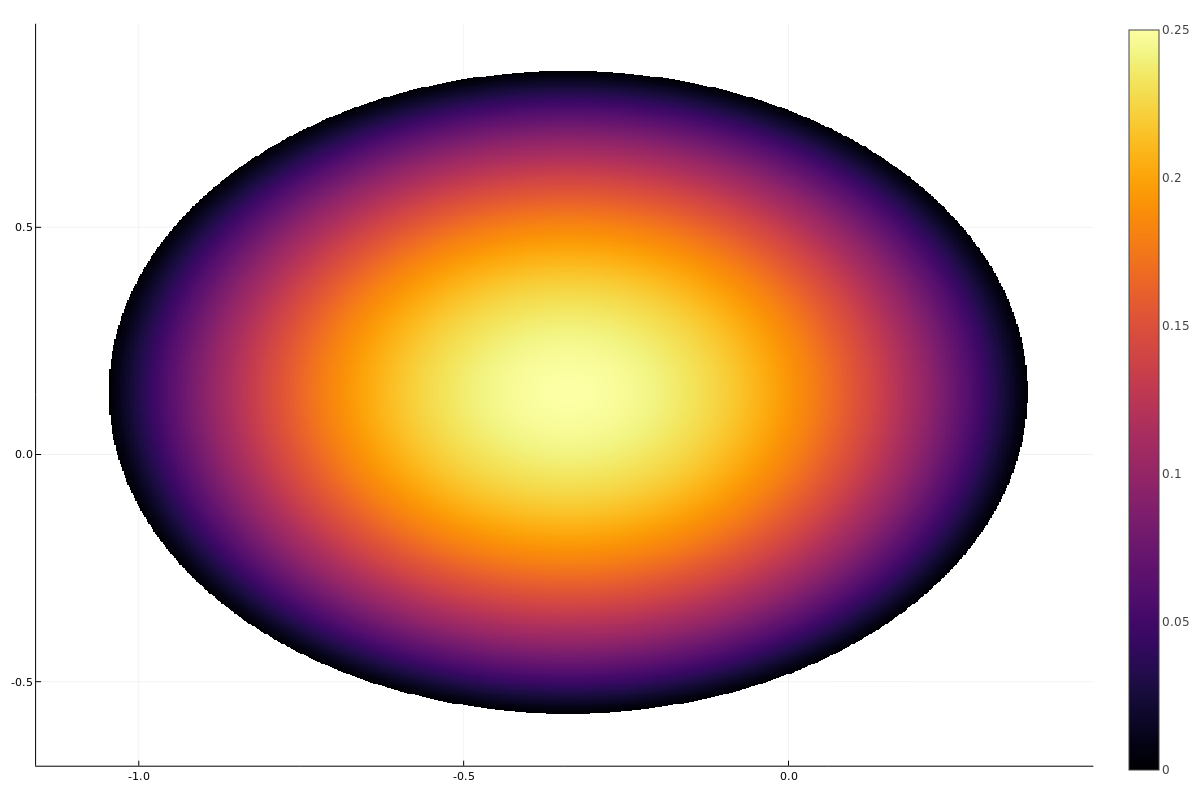
\includegraphics[width=0.99\textwidth]{det2.png}
    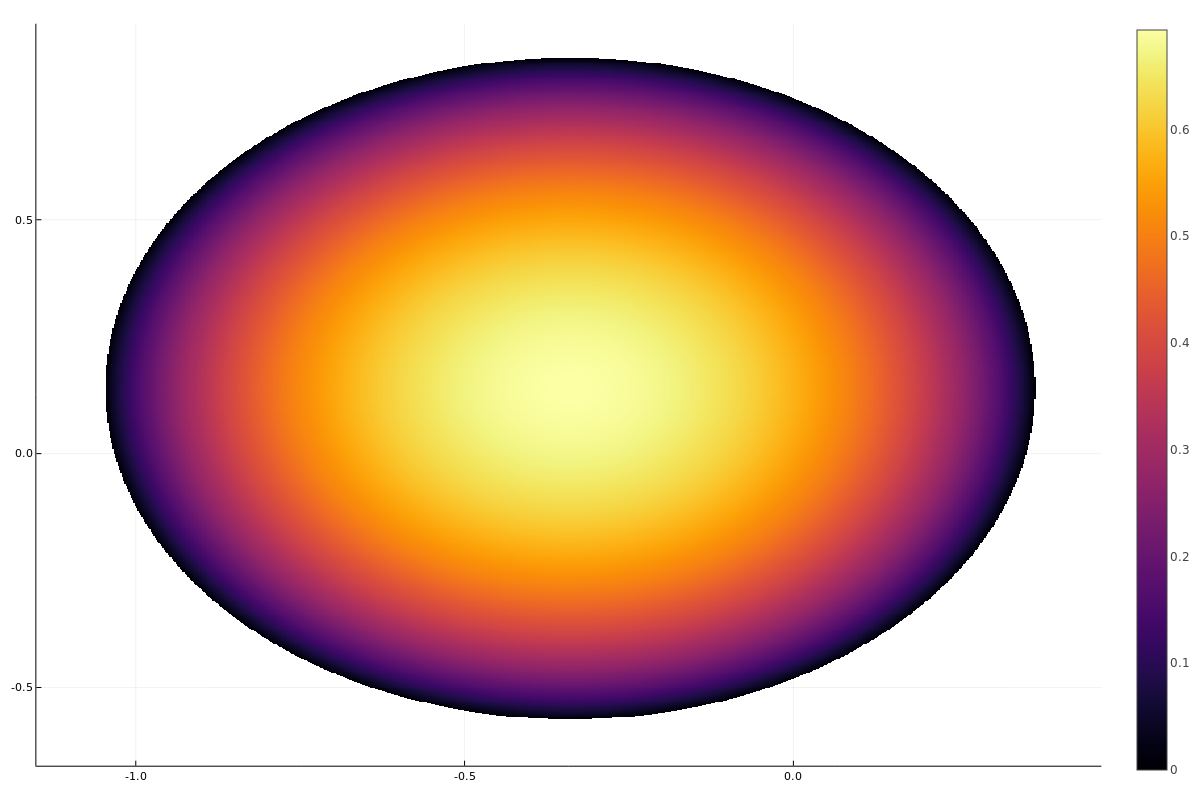
\includegraphics[width=0.99\textwidth]{ent2.png}
    \caption{dimension 2}

  \end{subfigure}
  \begin{subfigure}[t]{0.49\textwidth}
    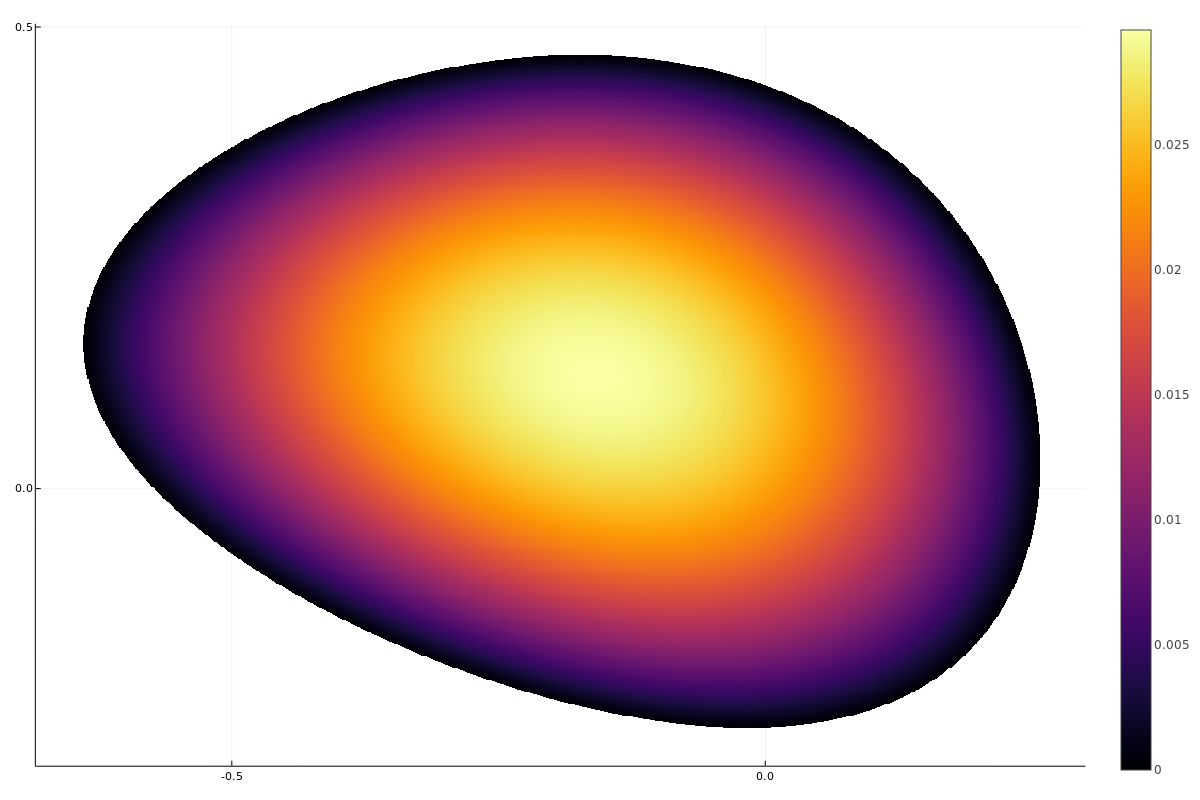
\includegraphics[width=0.99\textwidth]{det3b.png}
    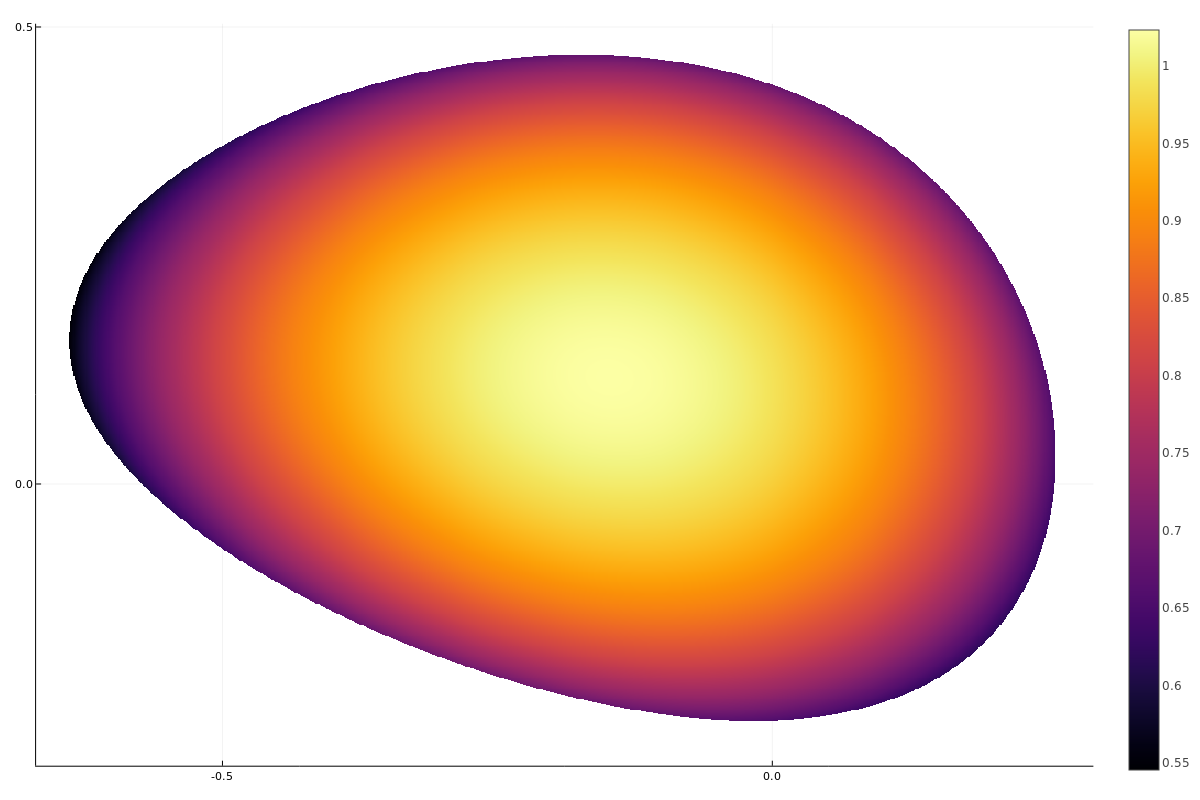
\includegraphics[width=0.99\textwidth]{ent3b.png}
    \caption{dimension 3}
  \end{subfigure}
  \begin{subfigure}[t]{0.49\textwidth}
    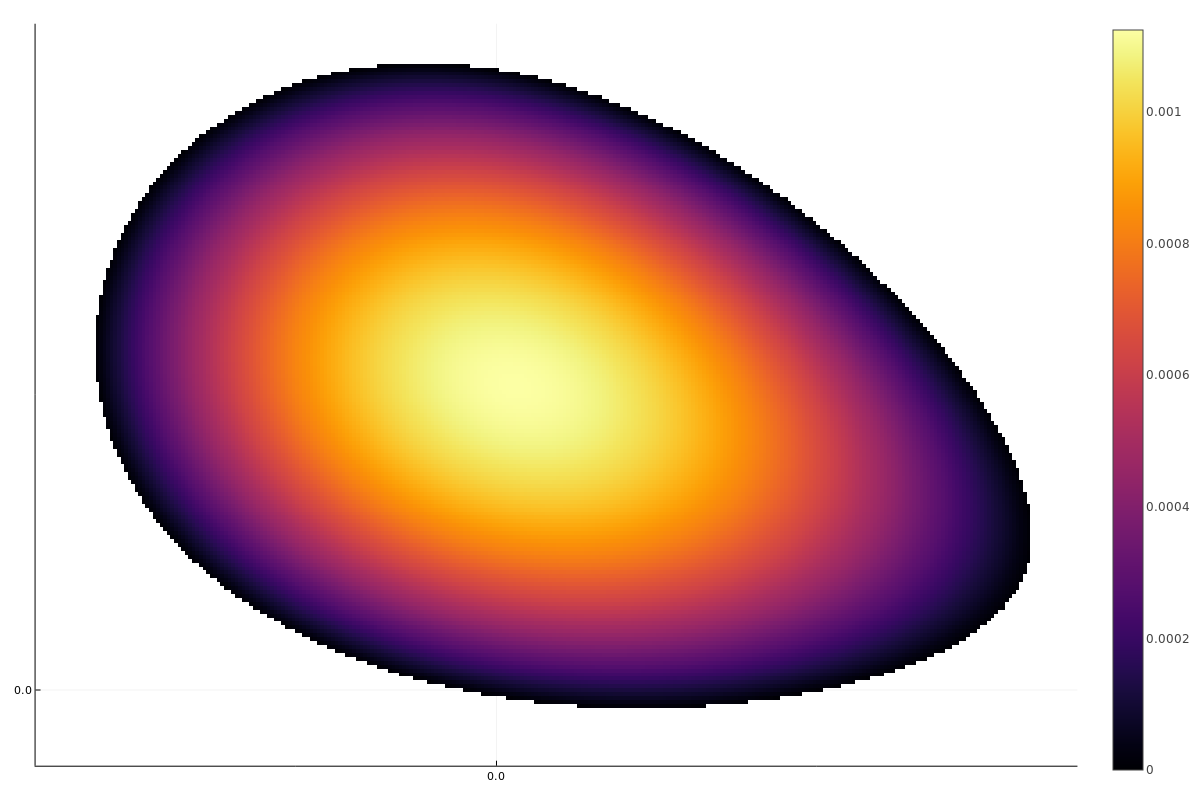
\includegraphics[width=0.99\textwidth]{det4.png}
    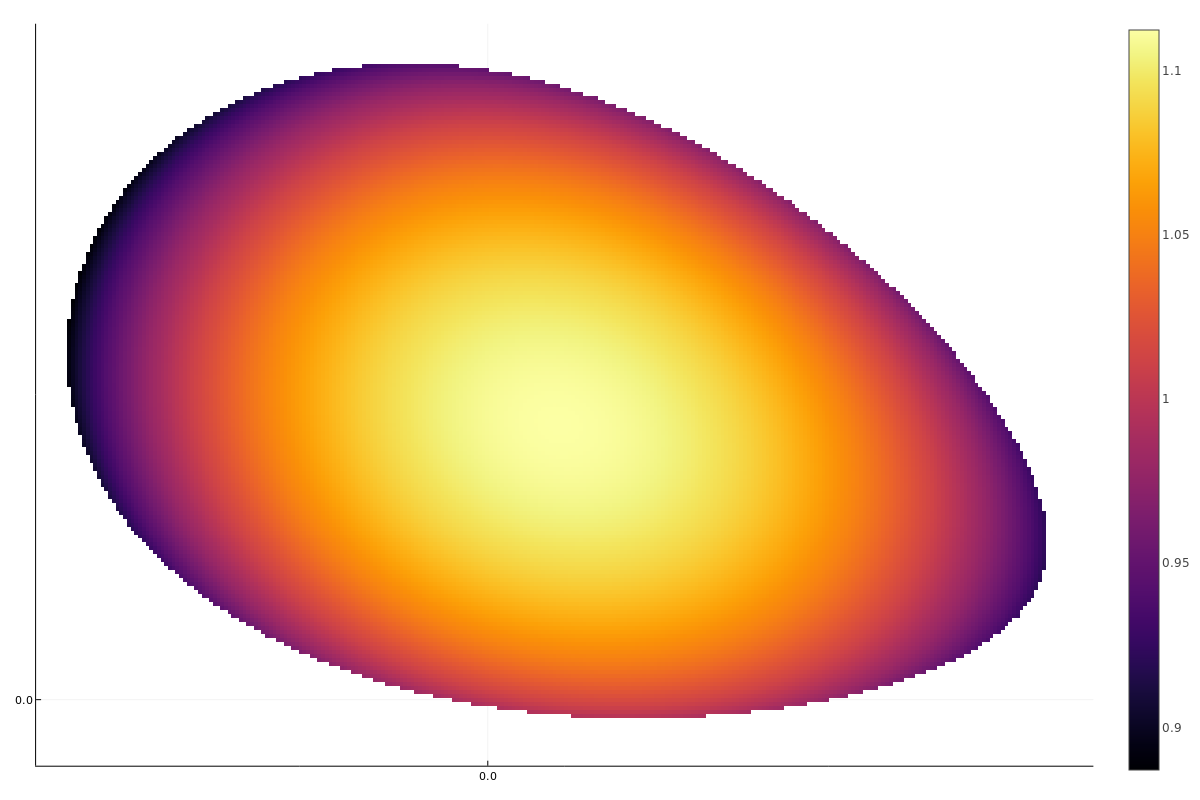
\includegraphics[width=0.99\textwidth]{ent4.png}

    \caption{dimension 4}
  \end{subfigure}
  \begin{subfigure}[t]{0.49\textwidth}
    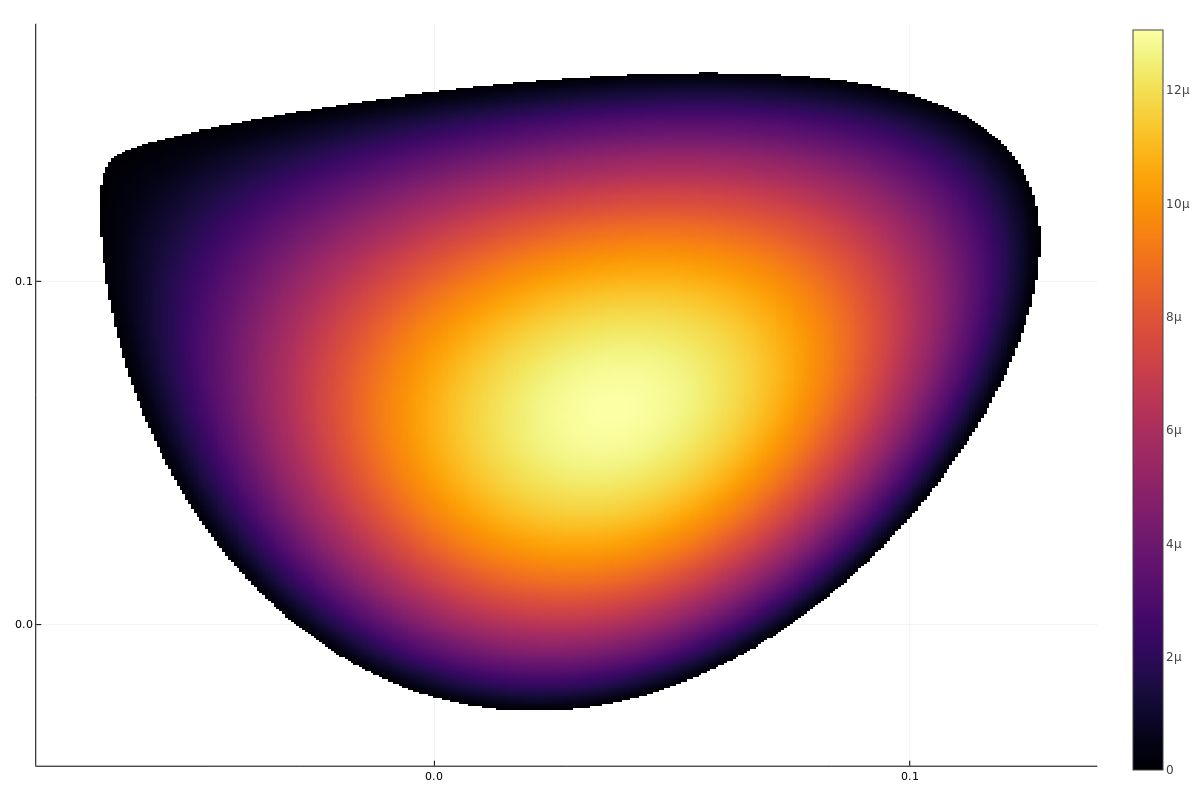
\includegraphics[width=0.99\textwidth]{det5.png}
    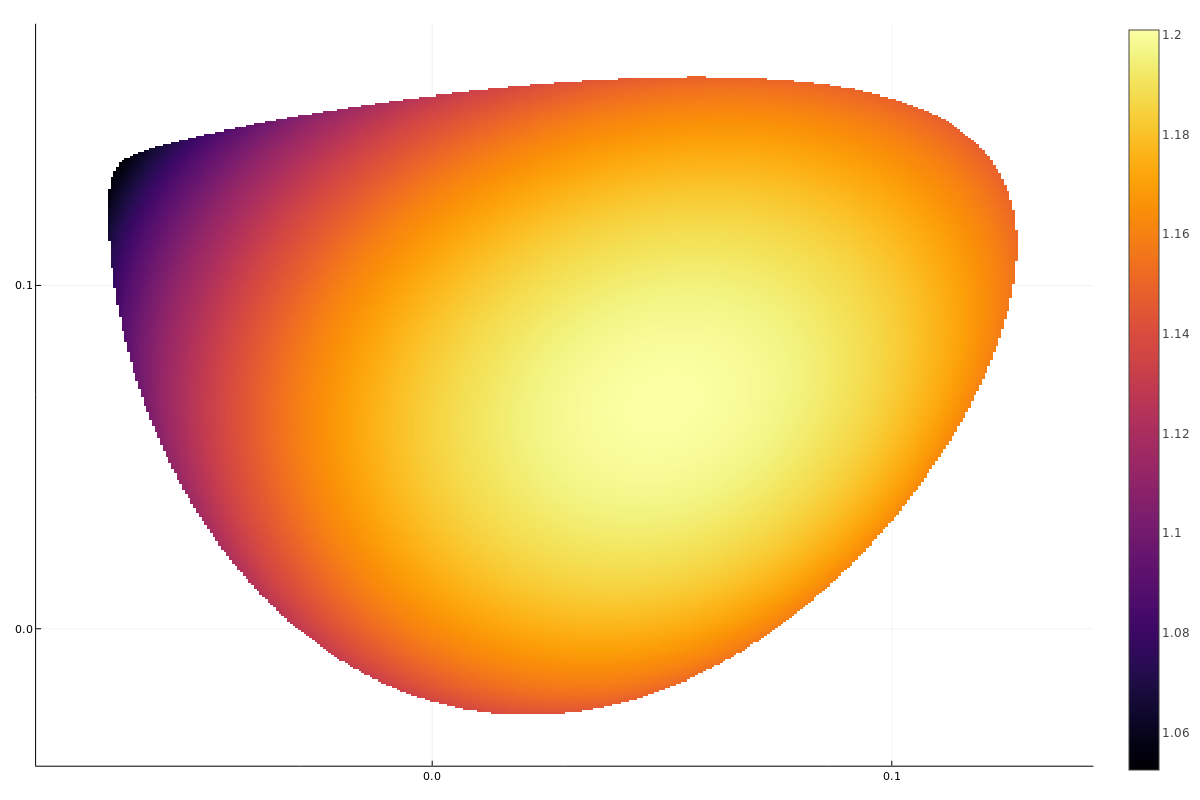
\includegraphics[width=0.99\textwidth]{ent5.png}
    \caption{dimension 5}
  \end{subfigure}

\caption{In order to compare $\log \circ \det$ and $S$, I plotted them on random affine planes
slicing $\mathcal{D}$. I pick a random density matrix $A$ and two random orthonormal null
trace matrices $H_1$ and $H_2$. I then plot $\log \circ \det$ and $S$ in the
plane $A + x H_1 + y H_2$. In each case $\log\circ \det$ is on top and the
entropy is below. The colorless area is outside of $\mathcal{D}$}
\label{fig:heat}
\end{figure}

\subsubsection{In practice}

That part of my work wasn't directly useful for Luis project, because his effect
matrices only span the population in Fock base and thus the centering simply
consists in putting $0$ in each correlation, which I think achieve perfect centering
whatever the centering function is.

\subsection{Two objective optimisation}

In odder to use the centering function, what we want to do is that, after
optimizing $\ell$ and landing on $M = \argmax_{\rho \in \mathcal{D}} \ell(\rho)$, we
can optimize the centering function on $M$ and get the most centered matrix that
maximize $\ell$.

One way of doing it is to do exactly what I just said: Find a $\rho_{int}$ in
$M$ with a first optimization (projected gradient ascent will find one, even I
haven't proved it in \cref{sec:projgrad}). Then we could optimize $c$ on $M$.
However I have no idea how to project a vector on $M$: The projection method
described in \cref{ssec:proj} only works on the whole $\mathcal{D}$ because
$\mathcal{D}$ is unitary invariant which is generally not the case of $M$.

An other way of doing that is by using a kind of barrier method with $c$. By optimizing $\ell +
\varepsilon c$ and reducing progressively $\varepsilon$, we'll the right
$\rho\ml = \argmax_{\rho \in M} c$.

\begin{prop}
  If I name $\rho_\varepsilon$ the solution of:
  \[\maximf{\ell + \varepsilon c}{\rho \in \mathcal{D}}\]

  Then, if $c$ is strictly concave, and uniformly continuous we'll have:

  \[ \rho_\varepsilon \xrightarrow[\varepsilon \to 0]{} \rho\ml = \argmax_{\rho \in M} c\]
\end{prop}

\begin{proof}
  Let's define $\ell\ml = \ell(\rho\ml)$.
  $\ell$ is strictly concave on all the dimension of which there is an $E_i$
  i.e all the dimension orthogonal to the $M$. That means that if
  $\ell(\rho_\varepsilon) \to \ell\ml$, then $d(\rho_\varepsilon,M) \to 0$.

  Then lets prove that $\ell(\rho_\varepsilon) \to \ell\ml$. We now that
  $\ell\ml > \ell(\rho_\varepsilon)$, but we also know that
  $\ell(\rho_\varepsilon) + \varepsilon c(\rho_\varepsilon) \geq \ell\ml +
  \varepsilon c(\rho\ml)$. Therefore:
  \[\ell\ml - \ell(\rho_\varepsilon) < \varepsilon (g(\rho_\varepsilon) - g(\rho\ml))\]
  But $c$ is strictly concave so it has an upper bound. So when $\varepsilon \to
  0$, we have $\ell\ml - \ell(\rho_\varepsilon) \to 0$ and thus
  $d(\rho_\varepsilon,M)\to 0$.

  Let's name $\rho_{p\varepsilon}$ the projection of $\rho_\varepsilon$ on $M$.
  As $\rho_{p\varepsilon} \in M$, we have $g(\rho_{p\varepsilon}) < c(\rho\ml)$.

  By uniform continuity, $d(g(\rho_{p\varepsilon}),c(\rho_\varepsilon)) \to 0$
  and $g(\rho\ml)$ is between them so. $c(\rho_{p\varepsilon}) \to c(\rho\ml)$.
  But as $c$ is strictly concave, this must mean that $\rho_{p\varepsilon} \to
  \rho\ml$.

  On the other hand we had $d(\rho_\varepsilon,M) =
  d(\rho_\varepsilon,\rho_{p\varepsilon}) \to 0$, so in the end we have
  $\rho_\varepsilon \to \rho\ml$.
\end{proof}

This proof works perfectly with the entropy but not with the $\log \circ \det$
as isn't uniformly continuous. Furthermore, the projected gradient method won't
work directly with the entropy because when projecting on the edge, the gradient of the
entropy will be infinite. I think both of this problems have solutions, for
example when we are on the edge, only output the tangent gradient for the
entropy. However, the internship is finished, so I won't have the time to check
it properly.


\chapter{Final Results}

\section{Approximation and implementation of first order error propagation}


Now I have the operator $\mathbb H$, and I want to compute the standard
deviation on various functions that are mixture of classical observable
evaluation and entropy-related functions. For my function $h: \mathcal{D} \to
\R$, I know from previous chapter that its standard deviation is:

\begin{equation}\label{eqn:stddev}
  \sqrt{\Tr(\nabla h\pr\mathbb H\inv \nabla h\pr)}
\end{equation}

The problem is that the function I want to evaluate are complex and span
multiple files of source code. I would like a method to propagate the error
estimation through all the layers of the code, following the way function are
computed. In order to do that, let's look at a more generic way of propagating
errors.

Suppose we have a random variable $X \in \R^n$ and its covariance matrix $V_X$.
Suppose we take a function $f : \R^n \to \R^m$ such that $P(X \in \dom f) = 1$.
We would like to know the covariance matrix of $f(X)$.
If $X$ has a probability distribution centered on its expectation $X_0$, such as
a normal law, We can make a first order approximation and assume that $f$ on the
domain where $X$ varies looks like $f(X_0) + \nabla f \cdot (X-X_0)$. In such a
situation one can prove that:
\begin{equation}\label{eqn:propag}
  V_{f(X)} = \nabla f^t V_X \nabla f = \bra {\nabla f} V_x \ket {\nabla f}
\end{equation}


This really looks like the \cref{eqn:stddev}. In fact if we linearize our
Hermitian matrices $\nabla h$
and thus think of $\mathbb H$ as an element of
$\mathcal{L}(\mathcal{O}(\mathcal{H}))$, we can write:

\[V_h = \bra {\nabla h\pr} \mathbb H^{-1} \ket{\nabla h\pr}\]

Furthermore the projecting operator $\pr$ is linear and thus can be put in a
matrix form such that

\[V_h = \bra{\nabla h}P^t\mathbb H^{-1}P \ket{\nabla h}\]

In fact we have $P^t \mathbb H\inv P = \mathbb H$ but I don't need it so I
won't prove it. What is important is that $V_\rho = P^t \mathbb H\inv P$ looks
like the covariance matrix of $\rho$ around $\rho\ml$ and that I proved in the last chapter
that the first order error propagation gives the right asymptotic variance of
any function.

Therefore, in the code, I compute $V_\rho$ from the results of the
reconstruction and then when a function is applied one variable I compute its
covariance matrice with \cref{eqn:propag}. In the end when a function has a
single dimension output, the variance matrix is a simple variance real that I can put
through a square root to get the standard deviation on that value.

\section{Plots}

Here are the plots of \cref{sec:res1} upgraded with the new error bars.
Unfortunately I didn't have enough time to finish implementing the error
propagation of last section, so those value come from the Monte-Carlo algorithm.
We added several new points of data in between. The horizontal error bars are
due to Luis and are originated from imperfections in the control and measurement of the
temperatures of both the cavity and the atom.



\begin{figure}
  \centering
  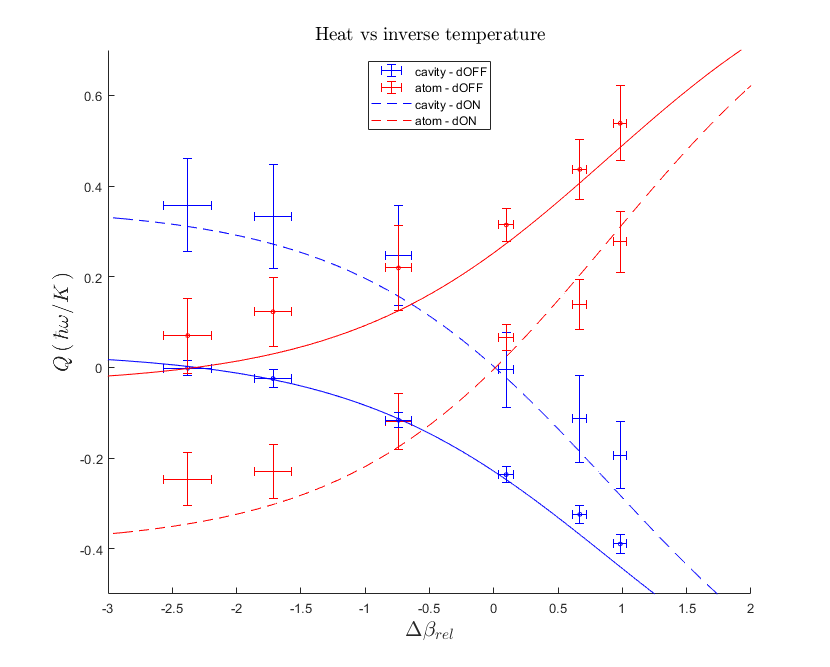
\includegraphics[height=0.45\textheight]{plots/Heat2.png}
  \caption{Plot of the exchanged heat depending on the Maxwell demon state ($ON$
    or $OFF$)}\label{fig:heat2}
\end{figure}

\begin{figure}
  \centering
  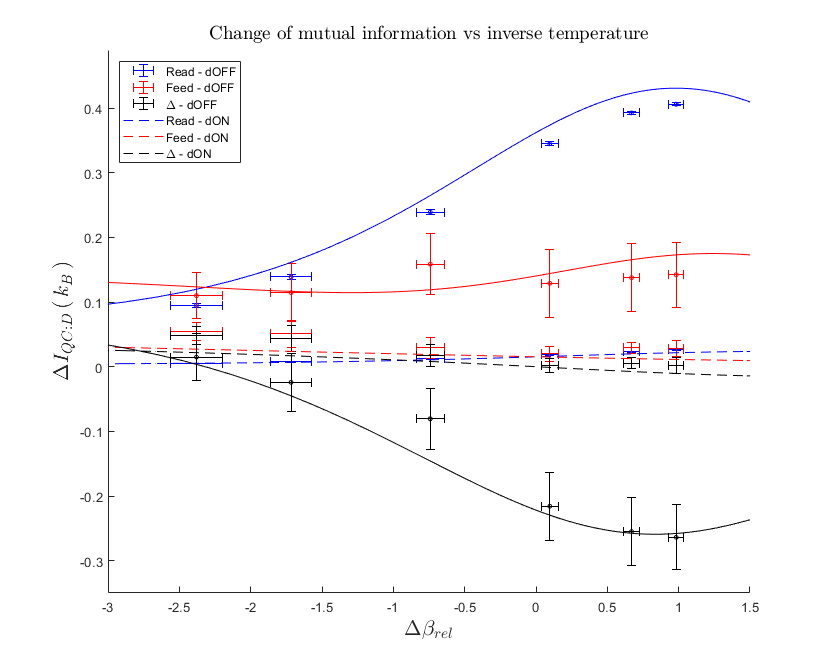
\includegraphics[height=0.45\textheight]{plots/Info2.png}
  \caption{Plot of the mutual information in the readout phase vs the feedback
    phase}\label{fig:info2}

\end{figure}

\begin{figure}
  \centering
  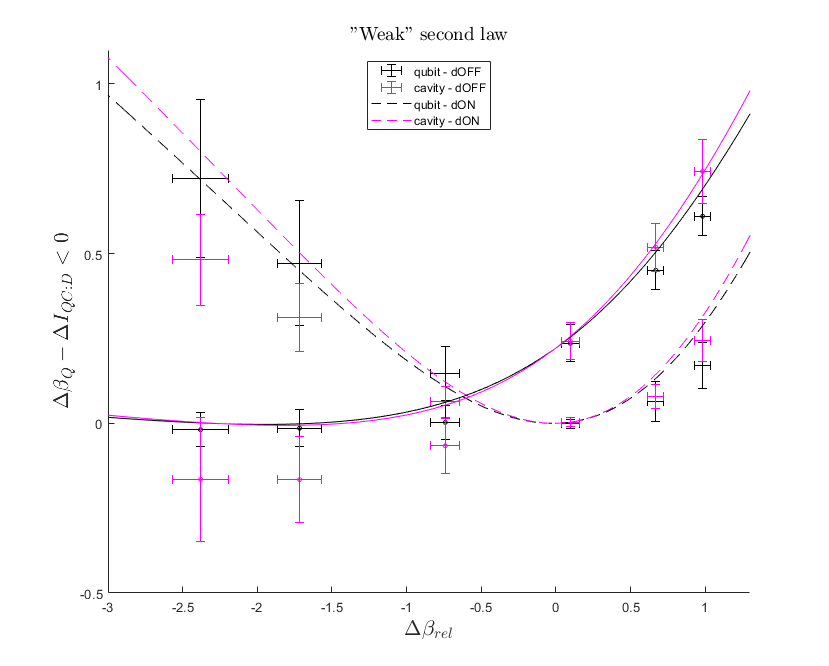
\includegraphics[height=0.45\textheight]{plots/Weak2.png}
  \caption{Plot of the weak second law in \cref{eqn:weaksnd}}\label{fig:weak2}
\end{figure}

\begin{figure}
  \centering
  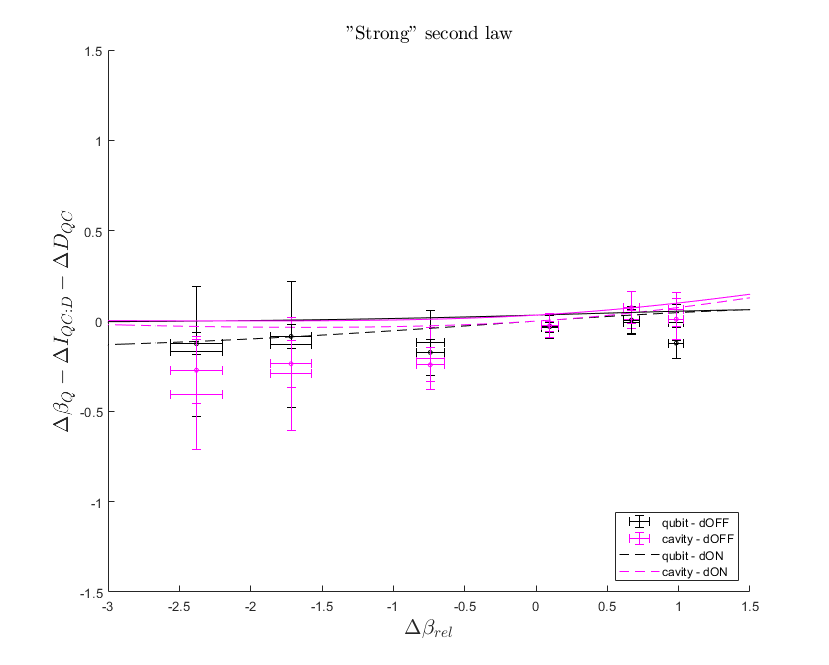
\includegraphics[height=0.45\textheight]{plots/Strg2.png}
  \caption{Plot of the strong second law in \cref{eqn:strgsnd}}\label{fig:strg2}
\end{figure}


\chapter*{Conclusion} %and bibliography
\addcontentsline{toc}{chapter}{Conclusion}

This internship was really interesting; I had to understand a lot of various
mathematical and physical theory to understand the huge amount of work that my
predecessor did. Once I did that I could have the pleasure to make a small but
nevertheless important
contribution to the field of quantum tomography.

It was really interesting to see the inner working of such a physics lab, and
to see the amazing experimental setup they have at the LKB. In particular to see
them running. Before
this internship I couldn't imagine that physicists were able to control atoms
and photons one by one to make experiments.

On a more theoretic point of view, this internship greatly improved my
comprehension of quantum mechanics both on the calculus side and the
interpretation side including my way of interpreting classical mechanics and
thermodynamics. It has also improved my knowledge on asymptotic integrals, but
that is a bit less prone to philosophy.

In the end, this was a great experience where I learnt a lot of things and met a lot
of interesting people, some of which I want to thank :

\vfill

\paragraph{\Huge Thanks}
\addcontentsline{toc}{chapter}{Thanks}

\

\vspace{1.3cm}

\begin{itemize}

\item Thanks to Igor Dotsenko for welcoming me in his lab, showing me their
  amazing experimental setup and giving me interesting things to do around it.\\
\item Thanks to Pierre Rouchon for giving me interesting corner-case problems to solve
  around log-likelihood maximization and helping me along the way when I was stuck.\\
\item Thanks to Luis Najera for having a great internship project thus allowing
  me to contribute to something very interesting. Thanks also to
  him for answering all my question about the codebase and helping me to
  implement some parts of my work. Also thank to him for answering various
  physical questions when I had trouble understanding quantum electro-dynamics or
  just quantum information theory.\\
\item Thanks to Valentin Metillon for helping me to understand various thing
  about physics and statistics.
\end{itemize}


\vfill

% Bibliography

% \addcontentsline{toc}{chapter}{Bibliography}

\bibliographystyle{plain}

\bibliography{report}

\addcontentsline{toc}{chapter}{Bibliography}

\addtocontents{toc}{\setcounter{tocdepth}{0}}
\appendix

\chapter{Quantum mechanics pictures}\label{app:pict}

Pictures are different way to perceive and express quantum mechanics. They vary
in how the system state and the various operator change over time. All those
representation yield the same mechanics and are equivalent up to certain change
of Hilbert space basis dependent on time. Going from one to the other is just up
to a unitary $U(t)$.

% However, non-unitary evolution like decoherence or external measurement
% cannot be moved like that because it is not inversible. Therefore such
% evolutions will always apply to the state.

\section{Schrödinger picture}

The Schrödinger picture is the usual representation of quantum mechanics. In
this context only the state of the system varies and the way to observe it do
not change. When the system evolves under Hamiltonian $H(t)$,
the various operators relevant to the system are constant (unless they vary
because of a external source which is not the system) and the
state follow the Schrödinger equation:
\begin{eqn}\label{eqn:schro}
\[i\hbar \frac{\partial \ket \Psi}{\partial t} (t) = H(t) \ket {\Psi(t)} \]
\end{eqn}

\begin{prop}
  If $H$ is constant over time, the solution of~\cref{eqn:schro} is:
  \[ \ket {\Psi(t)} = e^{-i\frac H\hbar t}\ket{\Psi(0)}\]
\end{prop}

On very important theorem that makes a link the Heisenberg picture is the
following:

\begin{thm}[Ehrenfest]\label{thm:ehren}
  \[\der{}t\langle A\rangle = \frac i\hbar\langle[H,A]\rangle + \left\langle\dpar
      A t \right\rangle\]
\end{thm}



\section{Heisenberg picture}

In the Heisenberg picture however, the state in $\mathcal{H}$, only correspond
to the initial state and represent the whole trajectory. However to measure an
observable a time $t$, you its expression $A(t)$ at this point in time. The
equation that rules this evolution is



\begin{eqn}
  \[\der At   = \frac i {\hbar}[H,A] + {\left(\dpar At \right)}_{\!\!H}\]
\end{eqn}

Here the $[\cdot,\cdot]$ is the commutator and the partial derivative is the
variation of $A$ due to external element out of the system (i.e.~the variation
of H in Schrödinger picture). This equation is actually the not-averaged version
of Ehrenfest theorem (\ref{thm:ehren})

\begin{prop}
  The Schrödinger picture and Heisenberg picture describe the same mechanics. In
  particular $\bra \Psi A \ket \Psi$ is the same for any operator in both pictures.
\end{prop}

\begin{proof}
  The value of the average in Schrödinger picture if given by Ehrenfest theorem.
  Let's compute the same average in Heisenberg picture. On the right side, the
  averaging give instantly the right hand of Ehrenfest theorem. We only have
  left to prove:
  \[ \left \langle \der A t\right\rangle = \der{}t\langle A\rangle\]
  But this is still true by linearity.
\end{proof}

In fact, The Schrödinger equation has general which is the unitary evolution
operator $U(t)$. From there, the evolution of the state in Schrödinger's picture
in $\ket {\Psi(t)} = U(t) \ket {\Psi(0)}$, whereas the evolution of a operator
in Heisenberg picture is $A(t) = U^\dagger(t)A_0(t)U(t)$, where $A_0(t)$
expresses the variation from external elements.

If the Hamiltonian is time-independent, $U(t) = e^{-i\frac H\hbar t}$

\section{Interaction picture}

Sometimes, in order to compare two phenomenon, it is useful to compare two
Hamiltonian in certain way. Usually, this is to compare the free evolution of a
system to the interaction with another system, this is why this is called the
interaction picture. Will split our Hamiltonian in two parts:
\[H = H_0 + H_1\]
In most case we'll try to keep $H_0$ time independent and simple, whereas $H_1$
will contain all the complexity of the system. That way, $U_0(t)$, will still be
$e^{-i\frac {H_0}\hbar t}$. We'll then make operator evolve with $H_0$, when
state evolves with $H_1$. The equations are:

\[i\hbar \frac{\partial \ket \Psi}{\partial t} (t) = H_1(t) \ket {\Psi(t)} \]
\[A(t) = U_0^\dagger(t)A_0(t)U_0(t)\]

This equivalent to manipulating state in a moving frame that moves according to
$U_0$. The Schrödinger frame would then be the fixed frame and the Heisenberg frame
would be the one that move exactly with the state.

\chapter{Covariance}\label{app:cov}

\section{Covariance and variance}

\begin{defn}
  Given two random vector $X \in \R^n$ and $Y \in \R^m$, we let the covariance
  matrix be defined by:
  \[\cov(X,Y) = {\big(\cov(X_i,Y_j)\big)}_{i \leq n, j \leq m}\]
\end{defn}

The fundamental goal of the covariance matrix is to have $\bra a \cov(x,y) \ket
b = \cov(a \cdot x, b \cdot y)$
\begin{prop} If $X \in \R^n$ and $Y \in \R^m$ are two random vectors, we have $\cov(X,Y) = {\cov(Y,X)}^t$.
\end{prop}
\begin{prop} If $A$ is a deterministic matrix, we have $ \cov(A X, Y) = A \cov(X,Y)$
\end{prop}

\begin{defn}
  Given a random vector $X \in \R^n$, We define its variance by
  \[V(X) = \cov(X,X)\]
\end{defn}

\begin{prop} For $X \in \R^n$a random vector, we have $V(X) > 0$
\end{prop}

\section{Correlation}\label{sec:correl}

\begin{defn}
  If $X$ and $Y$ are two real valued variable that are not fixed (non-zero
  variance), we have:
  \[\rho = \left|\frac {\cov(X,Y)}{\sigma(X),\sigma(Y)}\right|\]
  where $\sigma(X) = \sqrt{V(X)}$
\end{defn}

\begin{prop}\label{prop:correl1}
  We always have: $|\rho| \le 1$
\end{prop}

We can extend the correlation to the multivariate case by setting
\[\rho = {V(X)}^{-\frac12}\cov(X,Y){V(Y)}^{-\frac12}\]
The norm of $\rho$ now becomes the symmetric part of the polar decomposition:  $|\rho|
= {(\rho\rho^t)}^{\frac12}$. We can now get the theorem that give the bound on the
correlation:

\begin{thm}\label{thm:correln}
  If $X \in \R^n$ and $Y \in \R^m$ are random vectors, and $V(Y)$ is invertible,
  we have:
  \[\cov(X,Y){V(Y)}^{-1}\cov(Y,X) \leq V(X)\]
\end{thm}

\begin{cor}
  If $V(X)$ is also invertible, we have $|\rho| < I$
\end{cor}

\begin{proof}
  We take $a \in R^n$ such that $\bra a V(X) \ket a > 0$ and any $b \in \R^m$.
  By using~\cref{prop:correl1}, we get:
  \[ \frac{ \bra a \cov(X,Y) \ket b}{\sqrt{\bra a V(X) \ket a}\sqrt{\bra b V(Y)
        \ket b}} \leq 1\]
  To saturate the inequality, we can maximize the numerator on $b$, but keep the
  denominator constant. If we use the Lagrange multiplier method, we want to
  find a critical point of:
  \[\mathcal{L}(b,\lambda) = \bra a \cov(X,Y) \ket b + \lambda \bra b V(Y) \ket
    b\]

  We thus need to have:
  \[ \bra a \cov(X,Y) + 2\lambda\bra b V(Y) = 0\]
  and thus:
  \[ \bra b = - \frac 1 {2\lambda} \bra a \cov(X,Y) {V(Y)}^{-1}\]
  By substituting in the first equation we get:
  \[ \frac{ \bra a \cov(X,Y) {V(Y)}^{-1} \cov(Y,X) \ket a}
    {\sqrt{\bra a V(X) \ket a}
      \sqrt{\bra a \cov(X,Y) {V(Y)}^{-1} \cov(Y,X) \ket a}} \leq 1\]
  We thus get for all $a$ such that $\bra a V(X) \ket a > 0$:
  \[ \bra a \cov(X,Y) {V(Y)}^{-1} \cov(Y,X) \ket a < \bra a V(X) \ket a\]
  As for other $a$, both terms are 0, this inequality holds for all $a$, thus
  the theorem holds.
\end{proof}




\chapter{Some useful calculus}


\begin{equation}\label{eqn:gaussdimn}
  \int_{z \in\R^n} e^{-\frac N2 \|z\|^2} \dd z = {\left(\frac
      {2\pi}{N}\right)}^{\frac n 2}
\end{equation}
\begin{equation}\label{eqn:gausspown}
  \int_{r \in\R_+} r^{n+1} e^{-\frac N2 r^2} \dd r = 2^{\frac n2}N^{-\frac n2
    -1}\Gamma\left(\frac n 2 + 1\right)
\end{equation}

On integers, we have a simple value for the gamma-like integral:

\begin{equation}\label{eqn:gamma}
  \int_{r \in\R_+} r^{m} e^{- N r} \dd r = m! N^{-m-1}
\end{equation}



\begin{lem}\label{lem:gausssymtr}
  Let $S$ be an real symmetric matrix of dimension $n$, we have:
  \[\int_{z \in \R^n} \bra z S \ket z e^{-\frac N 2 \|z\|^2} \dd z =
    \frac{\Tr(S)}N {\left(\frac
        {2\pi}{N}\right)}^{\frac n 2} \]
\end{lem}
\begin{proof} If we take the spectral decomposition of $S$ and split the
  coordinate along $S$ eigenvectors, the result comes after some calculus.
\end{proof}

\section{Morse lemma}

\begin{lem}\label{lem:dec}
  Let $f : U \subset \R^n \to \R^m$, be $\class{n}$ with $U \in \mathcal{N}(0)$.
  Suppose that $f(0) = 0$. Then we have $g : U \to \mathcal{L}(\R^n,\R^m)$ of
  class $\class {n-1}$ such
  that:
  \[f(x) = g(x) x\]
  and with $g(0) = \nabla f(0)$
\end{lem}

\begin{proof}
  $g(x) = \int_0^1 \nabla f(tx) \dd t$
\end{proof}

\begin{lem}\label{lem:dec2}
  Let $f : U \subset \R^n \to \R$, be $\class{n}$ with $U \in \mathcal{N}(0)$.
  Suppose that $f(0) = 0$ and $\nabla f(0) = 0$.
  Then we have $h : U \to \mathcal{S}(\R^n)$ (Symmetric matrices) of class
  $\class {n-2}$ such
  that $h(0) = \nabla^2 f(0)$ and:
  \[f(x) = \bra x h(x) \ket x\]
\end{lem}

\begin{proof}
  We apply \cref{lem:dec} on $f$ to get $g$, that we see as a gradient $g :U \to
  \R^n$. Then we apply it again on $g$ to get $h_0$, then we take the symmetric part:
  \[h = \frac{h_0 + h_0^t}2\]

  We also have: $h_0(0) = \nabla g(0) = \nabla^2 f(0) = h(0)$
\end{proof}


\begin{lem}[Morse lemma]\label{lem:morse}
  Let $f : U \subset \R^n \to \R$, be $\class{n}$ with $U \in \mathcal{N}(0)$.
  Suppose that $f(0) = 0$, $\nabla f(0) = 0$ and $\nabla^2 f > 0$.
  Then we have a neighborhood $V$ of 0 and $\psi : V \to \R^n$ of class
  $\class{n-2}$, a such that on $V$:
  \[f(x) = \|\psi(x)\|^2\]

  If $n \geq 3$, we can have $\psi$ a diffeomorphism with $\nabla \psi(0) = \sqrt{\nabla^2 f(0)}$
\end{lem}

\begin{proof}
  We take $h$ as in \cref{lem:dec2}. As $h$ is continuous, we can take $V$ such
  that $h > 0$ on $V$ ($h(0) = \nabla^2 f > 0$).

  We can then define $\psi(x) = \sqrt{h(x)} x$. With the square root being the
  $\class{\infty}$ square root on the positive definite matrices.
  If $n \geq 3$, then $h$ is $\class 1$, thus we have: $\nabla \psi(0) =
  \sqrt{h(0)} = \sqrt{\nabla^2 f(0)}$. As $\nabla^2
  f(0) > 0$, we have $\nabla \psi(0)$ invertible, so by local inversion theorem,
  we can reduce the size of $V$ to make $\psi$ a diffeomorphism on $V$.

\end{proof}




\addtocontents{toc}{\setcounter{tocdepth}{2}}
\end{document}
